\documentclass[11pt,a4paper]{report}

\usepackage[a4paper,
			twoside,
			left=1.5in,
			right=1.0in,
			height=9.0in,
			headheight=14pt]{geometry}
\usepackage{fancyhdr}
\pagestyle{fancy}
\cfoot{}
\fancyhead[LE,RO]{\thepage}

\usepackage{url}
\usepackage[utf8x]{inputenc}
\usepackage{ucs}
\usepackage{amsmath}
\usepackage{amsfonts}
\usepackage{amssymb}
\usepackage{graphicx}
\usepackage{natbib}
\usepackage{multicol}
\usepackage{subcaption}
\usepackage{makecell}
\usepackage[hidelinks]{hyperref}
\usepackage{rotating}
\usepackage[toc,page]{appendix}
\usepackage{epstopdf}
\usepackage{caption}
\usepackage{subcaption}
\newcolumntype{"}{@{\hskip\tabcolsep\vrule width 1pt\hskip\tabcolsep}}


% Code snippet setup ---- START
\usepackage{listings}
\renewcommand{\lstlistingname}{Snippet}
\usepackage{color}
\definecolor{dkgreen}{rgb}{0,0.6,0}
\definecolor{gray}{rgb}{0.5,0.5,0.5}
\definecolor{mauve}{rgb}{0.58,0,0.82}
\lstset{frame=tb,
  language=Matlab,
  aboveskip=3mm,
  belowskip=3mm,
  showstringspaces=false,
  columns=flexible,
  basicstyle={\small\ttfamily},
  captionpos=b,
  numbers=left,
  numbersep=5pt,
  stepnumber=5,
  firstnumber=1,
  numberstyle=\tiny\color{gray},
  keywordstyle=\color{blue},
  commentstyle=\color{dkgreen},
  stringstyle=\color{mauve},
  breaklines=true,
  breakatwhitespace=false,
  tabsize=3
}
% Code snippet setup ---- END

\author{
	Christensen, Daniel\\
	\texttt{\href{mailto:dhch12@student.aau.dk}{dhch12@student.aau.dk}}
	\and
	Høeg, Emil Rose \\
	\texttt{\href{mailto:ehaeg12@student.aau.dk}{ehaeg12@student.aau.dk}}
	\and
	Lind, Rasmus Bloustrød\\
	\texttt{\href{mailto:rlind12@student.aau.dk}{rlind12@student.aau.dk}}
	\and
	Nilsson, Sam Alix \\
	\texttt{\href{mailto:snilss12@student.aau.dk}{snilss12@student.aau.dk}}
	\and
	Smed, Dina Madsen\\
	\texttt{\href{mailto:dsmed12@student.aau.dk}{dsmed12@student.aau.dk}}
	\and
	Sørensen, Casper\\
	\texttt{\href{mailto:csare12@student.aau.dk}{csare12@student.aau.dk}}
	\and
	Vinkel, Simone Patricia \\
	\texttt{\href{mailto:svinkel12@student.aau.dk}{svinkel12@student.aau.dk}}
}
\title{{\LARGE \textbf{Automatic Transcription of Beatboxing }} \\
{{\Large By group 403}}}


% BACKGROUND ---- START
\usepackage{eso-pic}
\newcommand\BackgroundPic{%
\put(0,0){%
\parbox[b][\paperheight]{\paperwidth}{%
\vfill
\centering
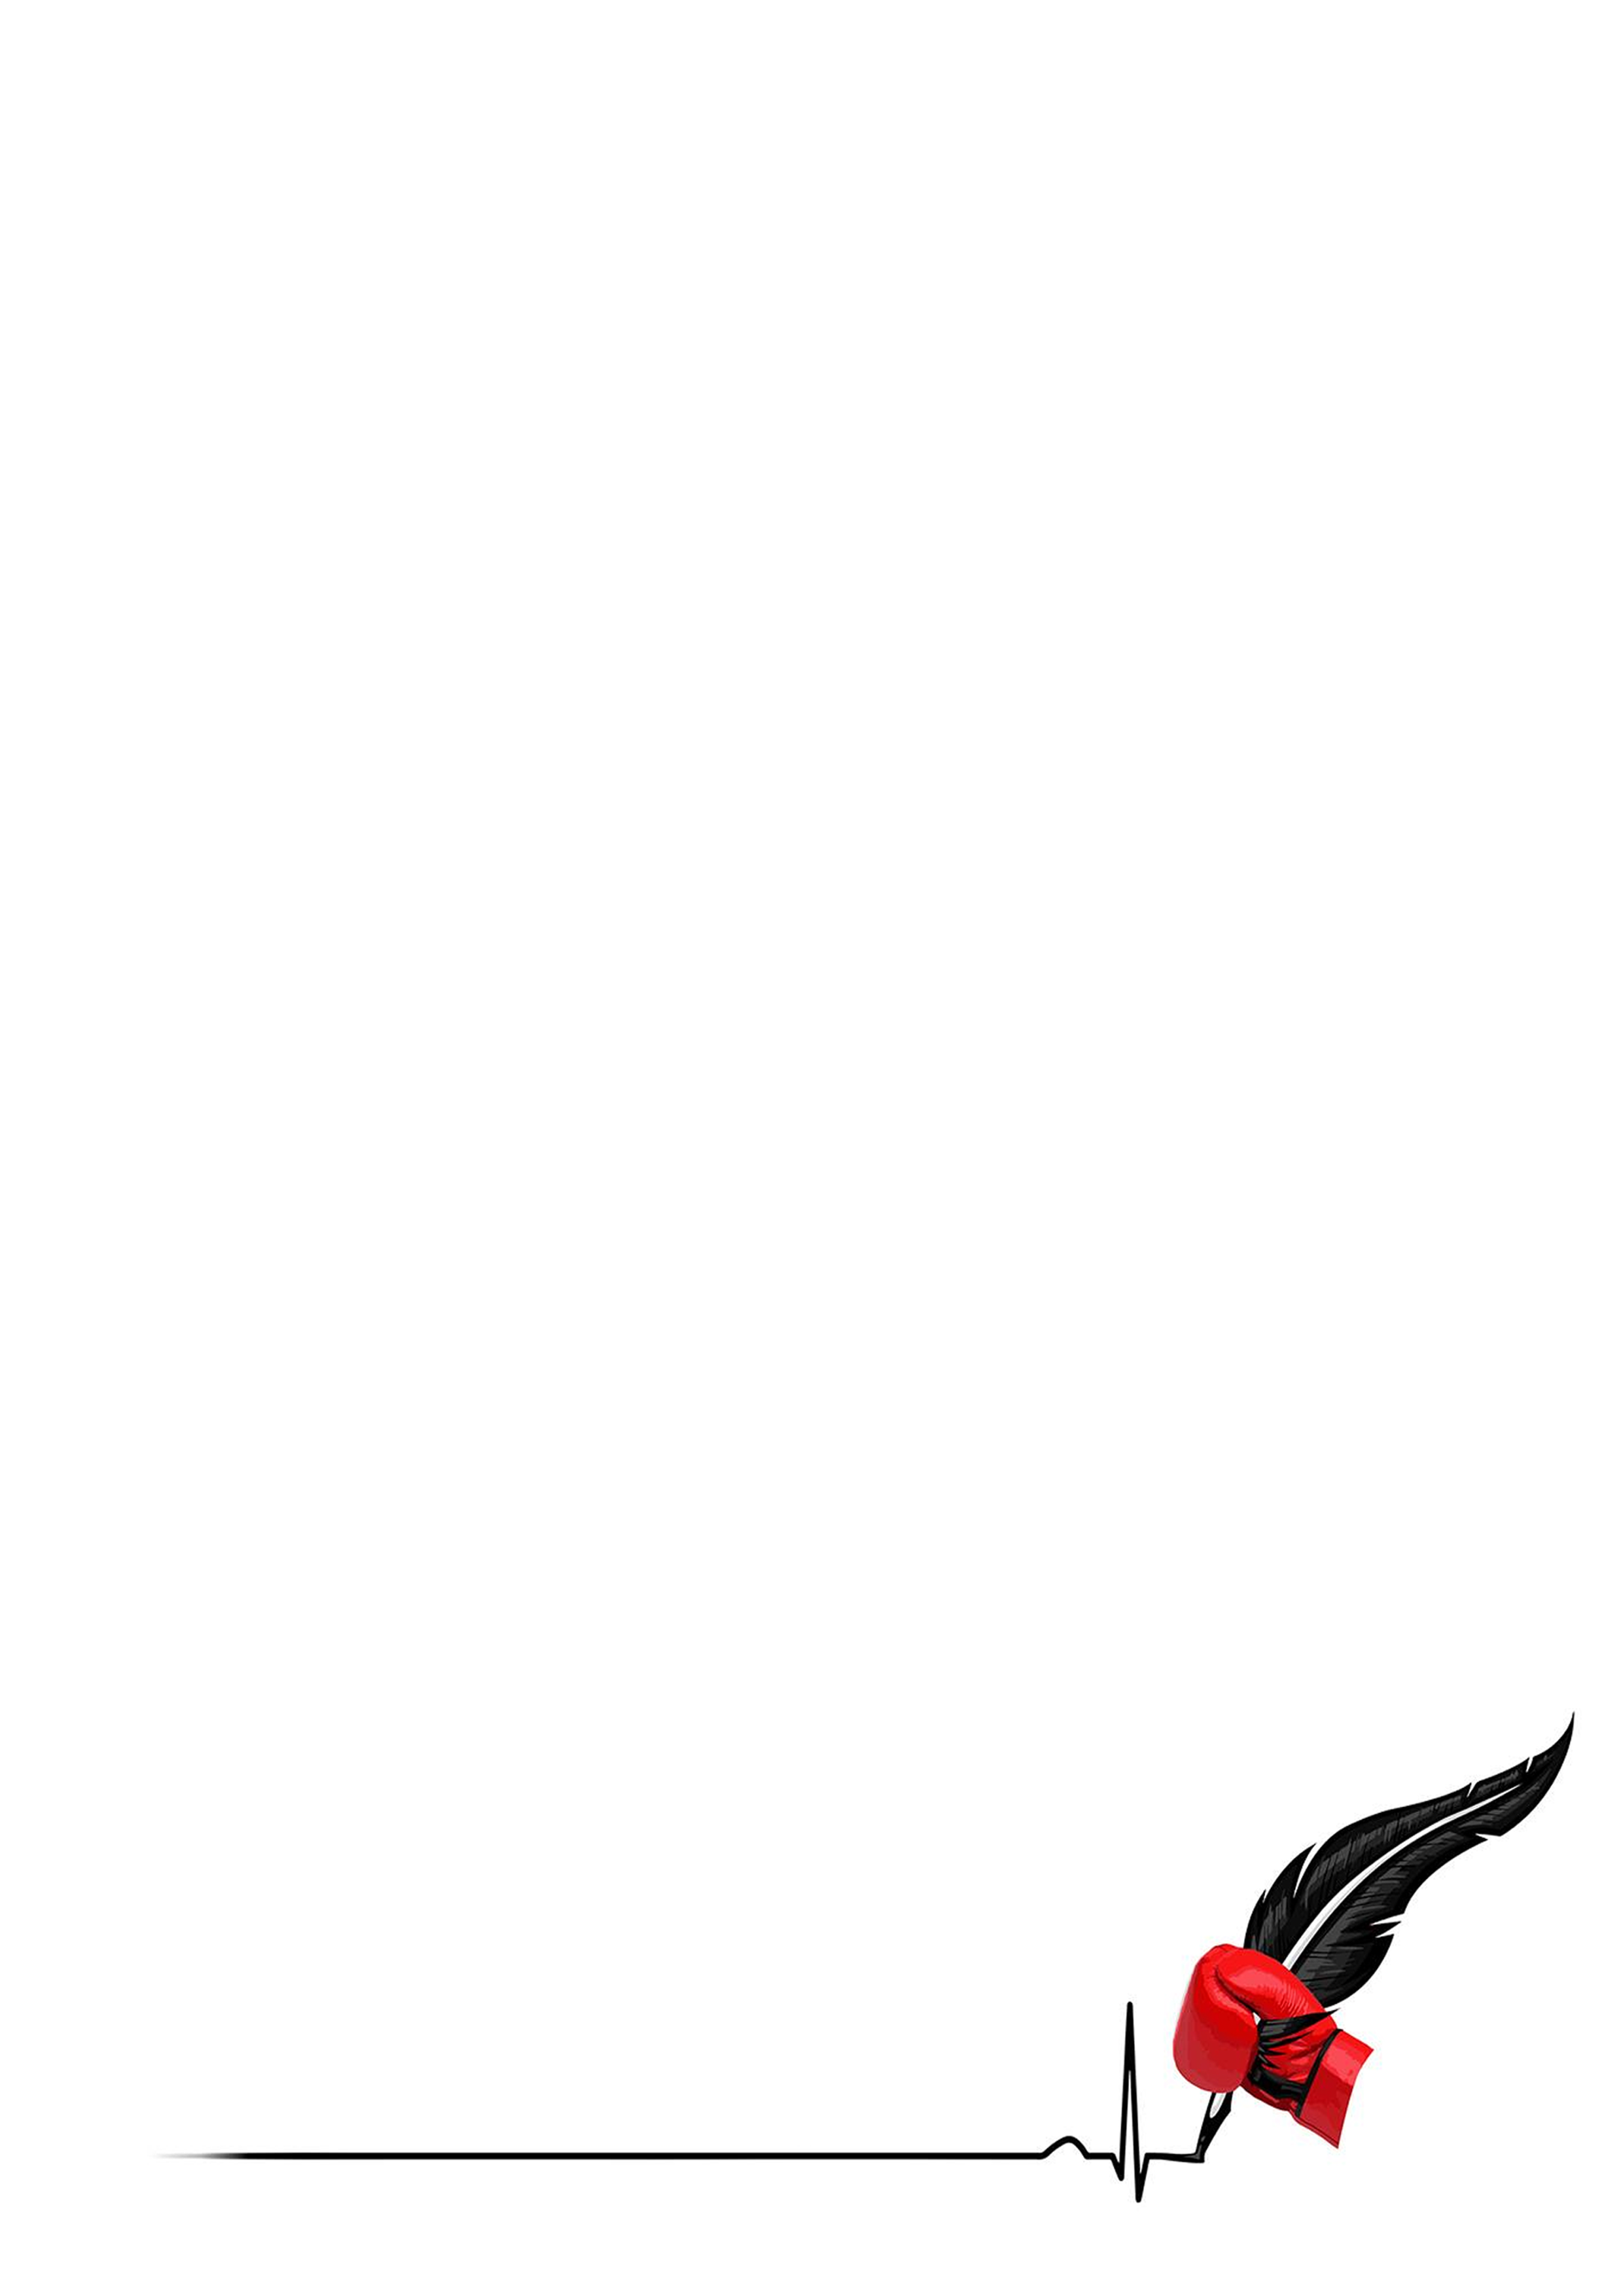
\includegraphics[width=\paperwidth,height=\paperheight,%
keepaspectratio]{fig/BBB2.png}%
\vfill
}}}
% BACKGROUND ---- END

\begin{document}
% Add background
\AddToShipoutPicture*{\BackgroundPic}

\maketitle
\tableofcontents
\chapter{Introduction}
\thispagestyle{empty}
Beatboxing is a tradition of vocal imitation of a percussionist playing a wide range of instruments to create a rhythmic and musical groove, and may be performed a capella or with amplifiying means \citep{Stowell2008}.
%Beatboxing originated in the 1980s, and is linked to the early hip-hop culture; it is also referred to as “the fifth element of hip-hop”. The self-proclaimed pioneer of Beatboxing, Doug E. Fresh also known as ‘The Human Beatbox’ was a key player in making Beatboxing famous \citep{Hess2007}. Earlier artists have been known to use similar techniques of vocal percussion in published material e.g. Paul McCartney with the song “That Would Be Something” from 1969.
%\footnote{\url{http://www.youtube.com/watch?v=VHTCWY7Lvpk&feature=kp}}.  
It is seen in different contexts: from a relatively primitive a capella performance style\footnote{Fatboys 1984: \url{http://www.youtube.com/watch?v=jJewbFZHI34}}, to a vocal percussive accompaniment to singing and rapping\footnote{Snoop Dogg 2004: \url{http://www.youtube.com/watch?v=RaCodgL9cvk}} , and also enhanced by technologies designed for stage and/or street performance\footnote{DUB FX with \textit{Love someone} from 2013: \url{http://www.youtube.com/watch?v=2xUnPhxHp3k}}.

With the first drum machines arriving, beatboxing emerged as a way for musicians to transcribe a drum beat into a vocalized percussive piece\footnote{"The Real History of Beatboxing": \url{https://www.humanbeatbox.com/forum/content.php/35-The-Real-History-of-Beatboxing-Part-2}}. Just like a musician can transcribe music, computer programs have been created to attempt to automatically transcribe a music signal into its notes. The idea of Automatic Music Transcription (AMT) was first proposed in 1977 by audio researchers James A. Moorer, Martin Piszczalski, and Bernard Galler \citep{Scheirer1998}, who considered the theoretical possibility to use computers to analyse a digital recording of music. Quite rightly the idea was executable, and has led to many computer programs who seek to automatically transcribe audio including music e.g. \textit{ Siri } on iPhone which answers to users' input or \textit{ Shazam } which recognizes songs. 
Automatic transcription of audio has shown its use in areas as diverse as biology such as bird type recognition, or video games like SingStar.
While transciption of audio sources has proven to be useful in many areas, interesting questions and aspects arise, if beatboxing could also be transcribed, and possibly used as MIDI controllers, instrumental karaoke, pedagogical purposes, and many more.
%These applications all share common features i.e. automatic retrieval of musical information and systems that offer an interactive music experience \citep{Benetos2012}. In continuation of this, AMT raises an interesting question: Can a beatboxing performance, likewise, be transcribed automatically? \\

% Standard Beatbox Notation (SBN) was developed by Gavin Tyte and Mark Splinter to create a simple and consistent method to aid novice beatboxers\citep{tyte2005}, through the use of percussive modelling synthesis with textual words \citep{McLean2009}. This method is also known as vocables \citep{McLean2009}.

%Vocables are intuitively a fast way to learn grooves and rhythms that will ultimately aid the novice beatboxer to improve his skills. However, SBN lacks a way in which the beatboxer can determine whether or not he succesfully used the right vocables to transcribe the corresponding percussive instruments. Maybe a software-based solution to automatically transcribe beatboxing, could be beneficial in alleviating this problem? A visual or audio system could plausibly  generate  the feedback required so the beatboxer can detect errors and omissions, and thus improve his or her skills.\\


Due to the fact that beatboxing is a subcultural phenomenon, there is very little substantial academic work done on the area \citep{Stowell2008}, but we have found several articles that propose possible solutions to beatboxing-transcription. Amaury Hazan created a beatbox controlled drum-machine \citep{Hazan2005}. Elliot Sinyor \textit{et al.} used the \textit{Autonomous Classification Engine (ACE)} to classify beatboxing sounds from a dataset he created with the help of 3 accomplished beatboxers and 3 non-beatboxers \citep{Sinyor05}. They further found that reducing the amount of classes to 3, they obtained a 98.15\% accuracy, versus the initial result of 95.55\% using 5 classes. Dan Stowell and Mark B. Plumbley approached the transcription with the goal of reaching real-time speeds \citep{Stowell2008}, by investigating delayed decision-making with various features. Together, the three papers touch upon a well of relevant knowledge on areas such as audio segmentation, audio features, classification, and system performance.

%Both papers advocate that delimitation is needed in relation to the number of different types of percussive sounds, ie. sound classes. 
%Although Dan Stowell and Mark D. Plumbley claims that neither of the projects are clear on whether they are developed in contact with practicing beatboxers \citep{Stowell2008},  Elliot Sinyor \textit{et al.} clearly describes that their test involved three beatboxers from an a cappella groups whereas two of them participate in beatboxing competitions.\citep{Sinyor05}. \\

In our project, we investigate automatic transcription of beatboxing. We create a dataset based on recordings of amateur beatboxers, which we test upon. We implement and evaluate audio features and classification, testing their performance with multiple varying parameters.
Furthermore we create an interface for easy analysis and classification of sounds (stored or recorded). Finally we use the results and experiences to discuss how our systems performance can be improved, and to further develop a useful tool for audio analysis.

%In this project, we explore the feasibility of automatic beatbox transcription, through thorough investigation inter alia of MFCC, spectral analysis, endpoint detection and the accompanying features. We design, implement a simple automatic beatbox transcription system as a proof of concept. We conduct several experiments on the system with acquired test statistic distributed between the training and test set in a 70\%/30\% ratio. The data will be evaluated using a Chi squared test to determine the optimal settings to identify the best performance. From these, we discuss how our system can be improved and might be expanded to other types of vocal percussion than beatboxing.\\

\paragraph{Structure of the report}\hspace{0pt}\\
The structure of this report is as follows: In the second section (Background), beatboxing is reviewed as an artform, the acoustic properties of chosen beatbox sounds i.e. hi-hat (hh), kick (k) and snare drum (s) are briefly discussed. Furthermore the tradition of other vocal music practices is contextualized with beatboxing to perspectivate the project. The third section (Methods of beatboxing-transcription) contains reviews of other approaches that have been designed for automatic transcription of beatboxing. State-of-the-art applications, features and proceedings are considered to provide insight into classification and transcription methods. In the fourth section (Our Approach), the design and implementation of our developed software solution are presented. In the fifth section (Evaluation), the evaluation of our system is presented in accordance with the aforementioned method. The sixth section (Discussion) stands in continuation of the preceding chapter, as the acquired results are discussed. Furthermore, in light of the results, avenues for future improvements of our system are suggested. The success of our system with respect to existing systems, and additional applications outside of transcription are discussed in the concluding section.
%\section{ Introduction }
\subsection{ Imitation of Instruments }
In the modern ages people have been imitating instruments for many reasons. One could be the need to describe or invent melodies, rhytms, tones and compositions, and being able to describe them to others. Another reason could be the lack of instruments or perhaps is tapping and humming simply the most intuitive ways to imitate rythms and melodies. Nevertheless is the act of vocalizing percussive sounds probably as old as music itself \citep{Sinyor05}.
\subsection{ Vocal Percussion }
Using mouth, lips and throat to produce percussion sounds and effects is seen in many cultures \citep{Sinyor05}. North American scat singing, mainly seen in jazz, by applying rythmic elements to singing nonsense syllables referred to as "onomatopeia", I.e. by Ella Fitzgerald and Louis Armstrong \citep{Janer_syllablingon}. Vocal imitation of percussion also comes in humorous variations as in the southern American predecessor to beatboxing called "Eefing", described as a "a kind of hiccupping, rhythmic wheeze". Known artists as Joe Perkins hit the charts in 1963 with the song "Little Eeefin' Annie" featuring Jimmie Riddle, who was acknowledged for his skills in the genre at the time \citep{jennifersharpe2006}.

 The voice has also been employed to imitate instruments for pedagogic purposes. For example to teach Cuban percussion, "Vayttari" Indian music, Peking opera and Japanese Noh flute \citep{Janer_syllablingon}.

The modern day equivalent is known as Beatboxing which is primarily linked to the early hip-hop-culture in the 1980s. The self-proclaimed pioneer of Beatboxing, Doug E. Fresh also known as ‘The Human Beatbox’ was a key player in making Beatboxing famous. However, other earlier artists have been known to use similar techniques of vocal percussion in published material e.g. Paul McCartney with the song “That Would Be Something” from 1969 \citep{Sinyor05}.
\subsection{ Beatboxing }
Beatboxing is generally limited to percussive sounds produced by the vocal cord and body (e.g. clapping) to imitate rhythms of a drumset i.e. snare drum, hi-hat, kick drums, cymbals etc. but some Beatboxers also imitates bass and guitar and occasionally combined with singing. An example of this is Michael Winslow, an American comedian, actor, and beatboxer probably best known for his ability to make sound effects with his voice in the movie Police Academy from 1984. Beatboxing as an artform was an outspring of the hip hop culture since the 1980s. It was shaped by musical technologies in context with its age, and through time it evolved to become a complex instrumental expression. In the origin of beatboxing it was meant to imitate grooves and beats but soon it utilized sounds like basslines, scratching, effects, noise, and almost every musical instrument and “filters”. –With improved techniques and sophisticated microphone technology beatboxing became a modern instrumental element in many music genres of today.
\subsection{ Software to transcribe instruments }
Since “modern beatboxing” evolved, it seems like technology is reclaiming it is technological importance. Some artists are beginning to transcribe instruments, adding filters and effects to beatboxing which takes the complexity of beatboxing even further. I.e. Dub FX, Benjamin Stanford from Australia, who samples sequences of vocal basslines, grooves and adds effects to them. Lately he re-recorded ‘Love Someone’ using Roland RC-505, a so called ‘Loop Station’, based on sequential recording of each track in instrumental compositions. [2] This way, he can perform on streets as one person, sounding as an orchestra. ** NEED TO WRITE MORE ON TRANSCRiPTION**
\subsection{ Motivation }
The motivation of this project is the admiration of innovative artforms and to explore the opportunities that arise from them. It is the fact that any analog instrument can be treated as a source for digital and electronic processing. Paradoxically beatboxing comes from imitating other analog instruments, but every other analog instrument is also victimized by digitalization. Jimi Hendrix pushed the creative scope of playing guitar, Jean Michel Jarre by playing piano and electronic drums. Why shouldn’t beatboxing be treated as an analog instrument as well? 
\subsection{ Why Beatboxing? }
The good thing about beatboxing is that it is under constant adaption to modern instrument technologies. It’s intuitively the fast way forward to learn grooves and rhythms. Beatboxing comes easy to many even though it requires one to let go of shyness, -like any other instrument. The good thing about beatboxing is that it comes relatively easy to many people. It only requires creativity to imitate sounds and instruments, while many people also tends to have the ability of humming with decent outcome. If technology can provide additional possibilities to facilitate the creation music that sounds good, it can be a fun way to learn the principles of rhythm and to produce satisfactory music, even that one does not know the basics or the techniques of a traditional instrument. 

\chapter{Background}
\thispagestyle{empty}
\section{Beatboxing as an artform}
Beatboxing as an artform was an out spring of the hiphop culture back in the 1980s. It was derived by vocally imitating drum-machines known as beatboxes e.g. the Roland TR808, which was often used in the production of Hip-Hop music, as a way to create grooves and beats using the mouth, nose and throat \citep{proctor2012}. The self-proclaimed pioneer of beatboxing, Doug E. Fresh also known as the "the Original Human Beatbox" was a key player in making beatbox famous. Other mentionable artists were Darren Robinson (Fat Boys), Biz Markie and Rahzel, who also shaped and improved the techniques used in beatboxing (kilde hess).

While beatboxing primarily involves the imitation of percussive sounds, other beatboxers attempts to imitate bass, guitar or other effects. An example of this is Michael Winslow, and American comedian, actor and beatboxer, probably best known for his ability to make sounds effects, e.g. imitation of phones or helicopters with his voice in the movie Police Academy from 1984\footnote{\url{www.imdb.com/title/tt0087928/?ref_=fn_al_tt_1}}. 

Through time beatboxing has evolved to become a complex instrumental expression and an artform which is constantly advancing and adapting to modern instruments and audio technologies \citep{proctor2012}. Take for example the beatboxer Tom Thum who authentically imitates the pounding techno-rhythm from within a night club at a TEDx conference\citep{TEDx}. With improved techniques and sophisticated microphone technology beatboxing is today an instrumental element in many music genres besides hip-hop, and has as an example been used in pop-music by The King of Pop Michael Jackson\citep{MJ}.

On an international plan the internet has contributed to the growing popularity of beatboxing, especially with the establishment of the Human Beat Box-community by Alex Tew , who subsequently created the first ever beatboxing convention\footnote{\url{www.beatboxconvention.com}} in 2003; a convention which succeeded in assembling beatboxers from all over the world\footnote{\url{www.humanbeatbox.com}}.
The community is also behind the first beatboxing tutorials that were published in 2003. Furthermore Gavin Tyte and Mark Splinter developed the Standard Beatbox Notation (SBN) as a simple and consistent method to describe sounds and rythms used in human beatboxing \citep{Tyte}.
\section{Other vocal music practices}

Besides hip hop, rhythmic vocal practices are seen in many cultures \citep{Sinyor05}. E.g. “scat singing”, mainly seen in jazz, by applying rhythmic nonsense syllables to singing. I.e. by Ella Fitzgerald and Louis Armstrong \citep{Janer_syllablingon}. Vocal music practices is also seen in many other contexts, such as practical, artistical and pedagogical purposes as described briefly in this chapter.
\subsection{ Artistic Purposes}
Vocal imitation of percussion also comes in humorous variations as in the southern American predecessor to beatboxing called "eefing", described as "a kind of hiccupping, rhythmic wheeze" \citep{jennifersharpe2006}. Among known artists was Joe Perkins who hit the charts in 1963 with the song "Little Eeefin' Annie" featuring Jimmie Riddle, and was acknowledged for his skills in the genre at the time  \citep{jennifersharpe2006}. Other examples are the northern India recitation of solkattu \footnote{\url{ www.youtube.com/watch?v=d1yN96ZDGm8}} known as “Konnakol” \citep{proctor2012}, and Celtic lilting and diddling\footnote{\url{www.youtube.com/watch?v=Rm_oaqW_qRM&list=PLUgNSFkRKerlocdy-qiC2Z879JlH-FfHe}} also have the characteristics of percussive elements \citep{proctor2012}.
\subsection{ Pedagogic Purposes}
Vocal emulation of instruments has also been employed for pedagogic purposes. For example to teach Cuban percussion, Indian music "Vayttari" , Peking opera and Japanese Noh flute \citep{Janer_syllablingon}. For drum notations “changgo” is used in Korea, as vocables for samul nori drumming, whereas Cuban conga players vocalize motifs as “guauganco or tumbao patterns” \citep{proctor2012}.
\subsection{ Compositional Roles }
There are many examples of vocal emulation of instruments as some of them are mentioned above. Beatboxing imitates the drum track and is therefore adaptable to many types of compositions, both as a solo element and as an accompanying instrumental element. Compared to other vocal artforms, in particular the artforms mentioned in this chapter, beatboxing can be said to be the most dynamic and evolving form of vocal percussion as it is based on imitation of all modern instruments. Compared to its predecessor “eefing”, beatboxing is less dominating in the rhythmic composition, where many of the other mentioned vocal artforms are also relatively dominant, and are preferably used as solo elements in compositions. Lastly, beatboxing is a relatively new performance style \citep{Stowell2008}, but it is still widely embraced in mainstream music as in the underground hiphop environment. Beatboxing imitates both humorous elements and pure a capella expressions, which makes it interesting to utilize in many contexts. 
As it is widely utilized in the mainstream music industry, and known by some generations in modern ages, it becomes interesting to develop even further or reinvent certain technical aspects for the performing artists and providers of music technology. Which can also be said to be the background and motivation of the further studies.
\section{Phonemes}
\label{SBN}
In this project the focus is to understand basic transcription of beatboxing, meaning that only kick, snare and hi-hat are researched throughout this study. In order to articulate the percussive vocal sounds in terminologies this study revealed mainly two important ways to do so, the International Phonetic Alphabet (IPA) \citep{ipa} and the Standard Beatboxing Notation (SBN), which are also briefly described in this chapter \citep{humanbeatboxing}.


Sounds can be described as “phonemes”. Although phonemes are not a focus of this project, it is still important to remember that beatboxing can be a complex artform, and one would need a comprehensive systematic approach which could be somewhat facilitated by understanding and utilizing aspects of the IPA \citep{ipa}, the SBN, or a combination of both.


We found the most relevant articulation of phonemes for this project to be the SBN, as it is actually based on a “simplified” approach to the IPA. The technical characteristics of the phonemes used for notations (phonetic approach) is the way to describe the sounds used for beatboxing, which basically have much in common with the IPA. \\


The four types of phonetic sounds in beatboxing \citep{BeatboxBible}:

  \begin{itemize} 
	\item Plosives

	
	\textit{Plosives are sounds where one stop the airway and release sound. Often used for kicks and snares.}
  
	\item Fricatives
	
	
	\textit{Fricatives are continuous sounds like “schhh”, “tsss”. Often used to imitate cymbals.}
	
	\item Clicks
	
	
	\textit{Clicks are more subtle sounds that are often used to imitate claps and snaps, but also subtle snares.}
	
	\item Oscillations
	
	\textit{Oscillations sounds are continuous sounds imitating synthesized instruments and robotic sounds like vibratos and alarms.}
\end{itemize}

Each of these four groups of sounds can be described into further detailed characteristics and potential utilizability in transcription of beatboxing, but the main purpose of this chapter is mainly to get acquainted with the techniques and articulations of the beatboxing sounds, and an idea of the phonetic complexity. This information could be useful when taking further steps towards the development of a complex transcription of beatboxing.
\begin{figure}[h]
	\begin{center}
		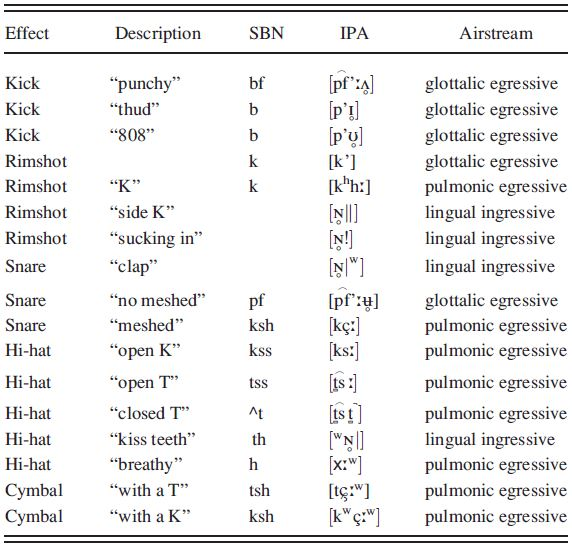
\includegraphics[height=5cm]{fig/phonemes.JPG}
		\caption{Illustration of phonemes utilized in Michael Proctors study on beatboxing \citep{proctor2012}}
		\label{VoiceBand}
	\end{center}
\end{figure}

%\section{Acoustic properties of beatboxing sounds}
The most basic and fundamental beatboxing sounds includes the ones imitating kick (also known as bass drum), snare and hi-hat of a drum-machine \citep{Stowell2010}. These sounds can be inspected through waveforms and spectrograms, in return for a better understanding of how the sounds relate and differ from each other. Below is a representation and description of the three mentioned sounds. \\

\begin{figure}[h]
	\begin{center}
		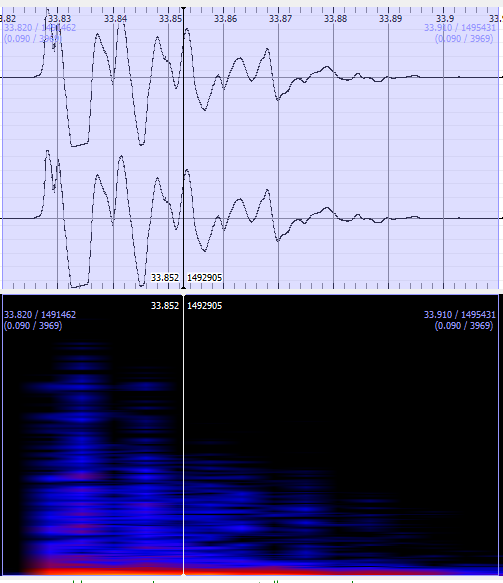
\includegraphics[scale = 0.5]{fig/Kick-closeup-with-spectrogram.png}
		\caption{Kick sound in waveform and in spectrogram (low frequency in the bottom of the spectrogram and high frequency in the top), made with Sonic Visualizer.}
		\label{KickClose}
	\end{center}
\end{figure} 

\begin{flushleft}
What can be seen on figure \ref{KickClose} is the kick sound. One can see that the kick sound has low frequencies, because the waveform does not cross the zero line that often, and in the spectrogram one can see more color in the bottom which is the low frequency.\\ 
\end{flushleft}

\begin{figure}[H]
	\begin{center}
		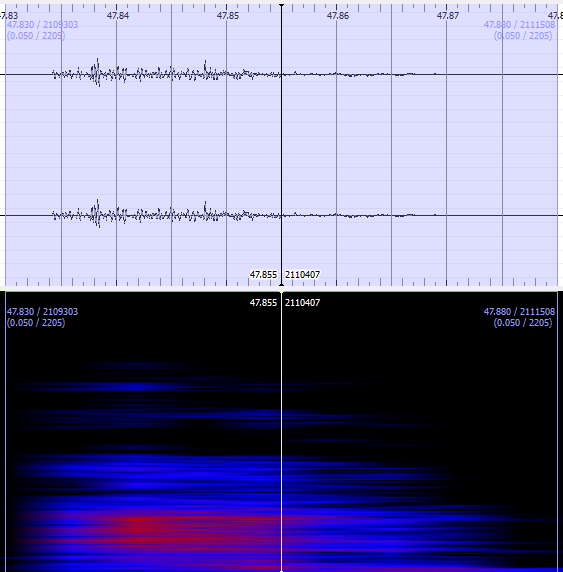
\includegraphics[scale = 0.5]{fig/Snare-close-up-with-spectrogram.png}
		\caption{Snare sound in waveform and in spectrogram (low frequency in the bottom of the spectrogram and high frequency in the top), made with Sonic Visualizer.}
		\label{snareClose}
	\end{center}
\end{figure}

\begin{flushleft}
Figure \ref{snareClose} presents a close up of the waveform of the snare sound. It can be seen that the sound has higher frequencies, and the spectrogram shows more colors closer to the top. 
\end{flushleft}
\begin{figure}[H]
	\begin{center}
		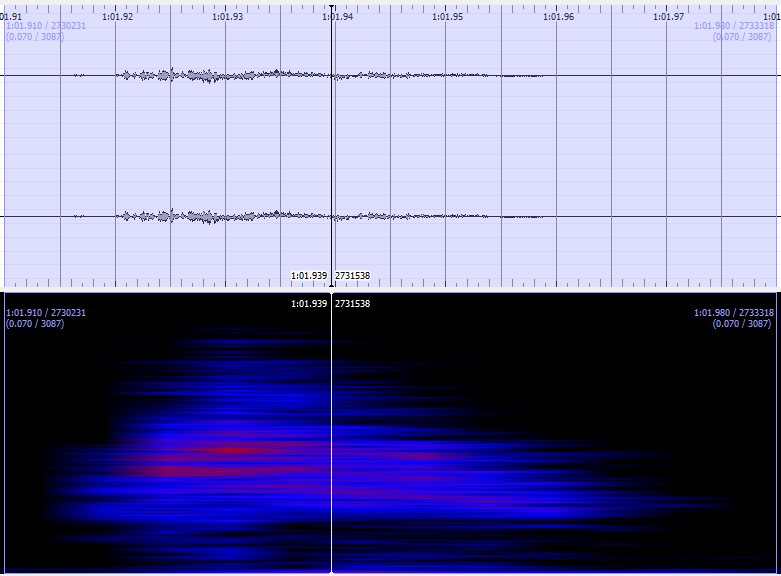
\includegraphics[scale =  0.5]{fig/HH-close-up-with-spectrogram.png}
		\caption{Hi-hat sound in waveform and in spectrogram (low frequency in the bottom of the spectrogram and high frequency in the top), made with Sonic Visualizer.}
		\label{HHClose}
	\end{center}
\end{figure}
Lastly, the hi-hat sound as seen on figure \ref{HHClose} has higher frequencies than the kick drum beatboxing sound. It also contains slightly higher frequencies than the snare drum. For an easier comprehension of the 3 sounds one can look at figure \ref{HH-Snare-Kick}.
\begin{figure}[H]
	\begin{center}
		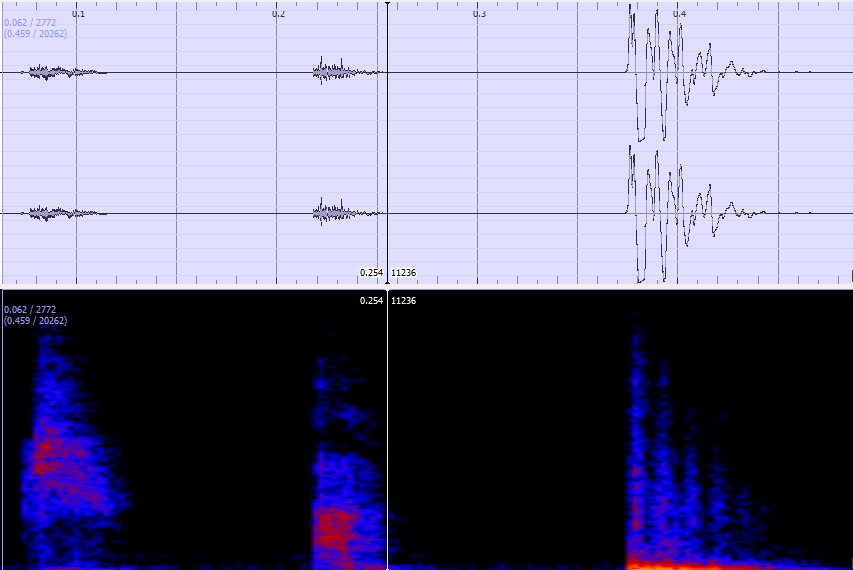
\includegraphics[scale =  0.5]{fig/hh-snare-kick-with-spectogram.png}
		\caption{Hi-Hat, snare and kick sound in waveform and in spectrogram(low frequency in the bottom of the spectrogram and high frequency in the top), made with Sonic Visualizer.}
		\label{HH-Snare-Kick}
	\end{center}
\end{figure}
What we can conclude from this is that the three sounds look different with the greatest difference in the kick compared to the snare and hi-hat.

\chapter{Applications and Technical Aspects of Beatboxing}
\thispagestyle{empty}
\section{intro}
This section will contain what works that are similar to the proposed problem of beatbox transcription that has been researched, first of some application that uses beatboxing or methods like beatboxing will be presented. Then some article that was found during research will be presented and the main point will be described. lastly some features that have been presented in the article will be described.
\section{ State-of-the-Art }
To comprehend the method of transcription, it is relevant to investigate software solutions and theoretical solutions that are approximate to the presented problem of this project. In this section the acquired solutions will be presented in conjunction with the presumed relevance which is necessary to solve the problem.
\subsection{ Eargram }
Most literature about concatenative sound synthesis is technically minded and focuses on the efficiency and use of the method. 
Eargram is a Pure Data patch with the main goal of utilizing machine learning to drive synthesis, using concatenative sound synthesis to combine analysed audio units into a coherent musical output (Bernades, Guedes, and Pennycook, 2012). Eargram was created as a larger application with many included tools, such as 4 different recombination methods and several visualization tools, and is architecturally heavily inspired by Skeleton (Jehan, 2005) and CataRT (Schwarz, Cahen, and Britton, 2008).
The authors mention that future development is much about the rhythm and correct recombination of separate audio units.

\subsection{ Voice Drummer }
Voice Drummer is defined as a "Percussion instrument notation interface" (Nakano, Goto, Ogata, and Hiraga, 2005). It is a software-application developed to aid those without substantial musical knowledge to notate music. The program is limited to transcribing bass drum and snare drum, and these are differentiated between by their onomatopoeic expressions and the rhythm-pattern timing.
\\
\begin{figure}[h]
	\begin{center}
		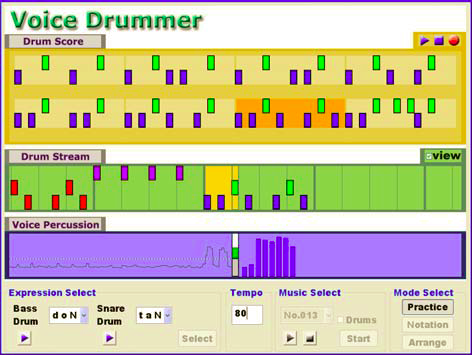
\includegraphics[height=5cm]{fig/VoiceDrummer.png}
		\caption{An example voice drummers practice adaption-mode}
		\label{VoiceDrummer}
	\end{center}
\end{figure}
\\
Onomatopoeic refers to words that phonetically imitates, or resembles the source of the described sound e.g. classifying 'Meow' as a sound a cat would make. Thus, making it easy for a layman to understand, and use Voice Drummer by uttering \textit{don-don} to generate a Bass Drum, and \textit{ta-ta} to generate a snare drum. These are transcribed into phonemic representations through a pronunciation dictionary which will recognize and
 output the correct corresponding output in real-time.

\subsection{ MATConcat }
In "MATConcat: An Application for Exploring Concatenative Sound Synthesis Using MATLAB"  By Bob L. Sturm, such an application has been made for Matlab. Here the method feature Concatenative sound synthesis is used, this methods will approximate a 'target' sound / input sound from a 'corpus' sound / database of sounds, the sound to use from the database is chosen from analysis of corpus sound and target to where they are matching most to some degree that can be set in the program (Sturm, 2004). The matching makes use of different parameters to make the choice of what is matching most. What degree of matching that the program will accept can be set in the interface and also what to do when the sound falls outside that degree (Sturm, 2004).

\subsection{ CataRT }
Another project called cataRT is using a similar method but in this project you can explore the analyzed data as they are shown in a space and as one navigates around in the space (cataRT, 2012). The space that one can navigate around in is comparable to what is described as the corpus or database in the MATConcat example, see figure0.1 for an better idea of how the interface looks like, this project is also implemented using a different platform that of maxMSP instead of MatLab.
\begin{figure}[h]
	\begin{center}
		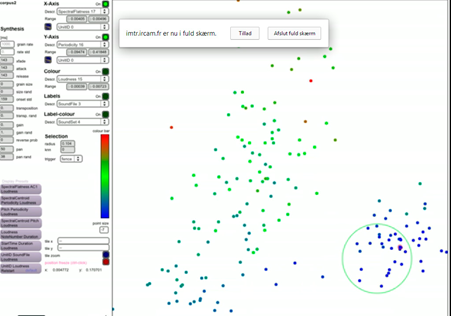
\includegraphics[height=5cm]{fig/cataRT.png}
		\caption{cataRT}
		\label{cataRT picture form video of cataRT showing the interface.}
	\end{center}
\end{figure} 
These methods could be using to make a voice imitate an instrument if a database was to be made with a given instrument, then by using this method it will be possible to analyze the input voice and find the closets sound from the database of the instrument sounds. Some analysis criteria would be needed to find the right database sound e.g. the pitch. 

\subsection{ Voice Band }
\begin{figure}[h]
	\begin{center}
		\includegraphics[height=5cm]{fig/voiceband.png}
		\caption{Voice Band}
		\label{VoiceBand}
	\end{center}
\end{figure}

Voice Band is an iPhone application by WaveMachine Labs which alters your voice into sampled instruments in real-time. It comes with a set of instruments to choose from including rhythm guitar, lead guitar, bass, sax, synthesizers, organ, drums and microphone, but there are other instruments and expansions available for purchase in the Voice Band store, e.g. other drum kits or strings. The target users are, according to WaveMachine Labs’ website and demo videos, songwriters who want an idea or arrangement down quickly; they call it a “portable musical scratch board”. However, it might also appeal and inspire anyone else interested in music, who wants to have fun. 

For every instrument, excluding the drums and cymbals, the system detects the pitch of the voice, and changes that into an instrumental output. To avoid distortion or unwanted noise, one will get the best results by using a pair of headphones, and staying in a quiet environment, because the system is very sensitive sound. It is also recommended to use solid, pure tones with no vibrato to reach a more accurate output, and to sing with hard consonants such as ba or da, because Voice Band recognizes the start of a sound, and it is therefore easier to detect.  

As for the drums, they are divided into kick/snare (two-in-one), hi-hat and crash. The kick and snare drums are together, where quiet will output kick, and loud notes will output snare. However there is the possibility to adjust the sensibility on a trigger in settings, such that only kick or only snare will be outputted, not depending on the loudness of the note. This way it is possible to record kick and snare separately as well. The hi-hat system works similarly in which soft notes produces a closed hi-hat and loud notes produces an open hi-hat. Crash is for itself. For all drums, and most of the other instruments, one can adjust reverberation and volume. 
All instruments and singing will have to be recorded separately, but on the same track. After having recorded an instrument, it will play back the previous recorded sounds while recording another one. It is possible to undo the last take without having to delete everything, but if you want to edit some of the first recordings this is not possible.  You cannot go back and change or edit the whole arrangement. It converts the samples into a MP3 file, which can be sent to an e-mail. 

\subsection{ Loop Station RC-505 }
The Roland Loop Station is specially build for beatboxers. It enables a performing beatbox artist to record and play 5 tracks simultaneously. It can also apply sound effects to the recorded tracks, which actually makes it sound closer to a synthesizer. The Loop Station can record 99 phrases, and provides 85 onboard rhytm patterns. Moreover it is can be operated with hands and with footswitches. Additionally it can be used as a MIDI controller. It has a XLR mic input, phantom power, mono/stereo instruments input, and AUX input, which makes the Loop Box stand out as one of the most professional build tools for beatboxers.

The Loop Station is used and promoted by the australian beatbox artist DUB FX.**SOURCE http://www.rolandconnect.com/product_2013-04.php?p=rc-505 **

\\
\begin{figure}[h]
	\begin{center}
		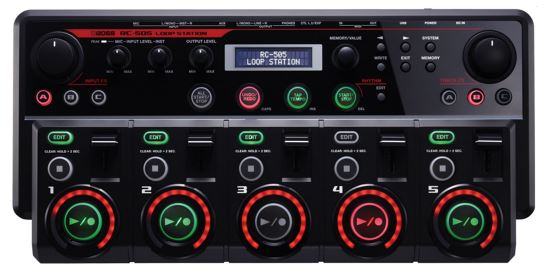
\includegraphics[height=5cm]{fig/Roland-RC-505.JPG}
		\caption{Roland Looper RC-505}
		\label{Looper}
	\end{center}
\end{figure}
\\

\section{Previous Work}
A great amount of effort has been put into investigating possible solutions to how transcription can be achieved through sound and music computing. While many articles, books and papers on the topic has been scrutinized, three specific articles we found to be of utmost importance to the project. The articles addresses relevant topics i.e. transcription - / and sound classification of beatboxing.

\subsection{Transcription}
In the article \textit{Towards Automatic Transcription of Expressive Oral Percussive Performances}, Amoury Hazan propose a solution to automatic transcription, that involves sound segregation, oral percussive descriptors, and machine learning techniques. Sound segregation is described as a simple method that fits well with monophonic oral percussive recordings, which requires few computing resources \citep{Hazan2005a}.	

His project aims to reduce the gap between the user and the device (keyboard, drum pad), among other things in order to offer an aid to those musicians who cannot transcript a beat they have in mind.
Through research of the taxonomy of human phonemes, and assuring perfect percussive events through segregation and transcription, the resulting drum score lack information concerning how the performer has modulated the produced sound. Thus, Hazan argues that energy and resonance frequency variation has to be defined together with effective computational methods to track them.
	
The considerations made by Hazan may serve as a benchmark tool which may suffice to serve as a possible solution to the problem. The technical descriptions and reflections could serve as an inspiration regarding how to construct the software based transcription-solution.

\subsection{Sound Classification}

[INSERT ARTICLE HERE - Beatbox Classification Using ACE \textit{by} \citep{Sinyor05} ]

It is important to understand how standard beatboxing techniques works, in order to build a system that recognizes vocal instrumental sounds. Each specific instrumental sound triggers the system to understand which sounds to replace with synthesized instruments. In this project the focus will be on basic percussion: kick, snare and cymbal.

The sequential process of classification contains 2 fundamental steps[**source**], to be described in this chapter: 

1.	Data Collection

	a)	Recording
	b)	Segmentation
	
3. Classification

	a)	Features
	b)	Feature Selection

Data Collection: 
Initially it is important to collect a range of sounds related to beatboxing. Therefore a dataset must be recorded both from experienced and unexperienced beatboxers. Subjects are instructed to record a small sequence of beatboxing, consisting of kick, snare and cymbal sounds (for this project). All sounds are recorded in 96Khz .wav files. 

** GRAPHICS DESCRIBING BASIC SAMPLES ** 

The recording for this project was done with a Zoom H4N linked to a standard phantom powered studio mic typically used by beatboxers. To get the most useful recordings the aim was to come as close as possible to the beatboxing sound environment, including background noise and the technical framework.


Segmentation:
Once all recordings has been collected

Classification: 





[INSERT ARTICLE HERE - Delayed Decisionmaking in real-time Beatbox Percussion Classification \textit{by} \citep{Stowell2010} ]

\section{Features}
\subsection{Root Mean Square}
The root mean square value is “the square root of the mean value of the squared values of the quantity over an interval"  \citep{Bird2007}.
\\
As Bird mentions in Engineering mathematics "One of the principal applications of RMS is with alternating current and voltage" \citep{Bird2007}. The alternating current (a.c.) is defined as a current which has a heating effect resembling the direct current \citep{Bird2007}.
\\
The RMS is found by doing these three steps:
(1) First take the square of the amplitude, (2) then take the mean of the squared results, (3) lastly take the square root of the results from the results of part (2) \citep{Bird2007}. \\ Here is \citep{Bird2007} mathematical formula for RMS:
\begin{equation}\label{eq:RMS formular}
RMS value = \frac{1}{b-a}\int_a^b\mathrm{y}^{2}\,\mathrm{d}x
\end{equation}

RMS tell us about the amount of energy used in the signal.

\subsection{Zero Crossing and Zero Crossing Rate}
Zero crossing is a term normally used in image processing, electronics and mathematics \citep{AlZhrani2010}. As explained by \citep{AlZhrani2010} in mathematics "“Zero-crossing” is a point where the sign of a function goes from negative to positive, or the other way around. This is represented by a crossing of the axis (zero value) in the graph of the function” \citep{AlZhrani2010}.
In other words zero crossing is a way of measure the period of a periodic signal aka the frequency \citep{RWW2012}. \\
When measuring a frequency, it is wise to measure an amount of periods instead of just one period. Since by having more periods can reduce errors caused by phase noise \citep{RWW2012} which is caused by making the perturbations (small pairs of zero crossing in regions of low energies \citep{Mallat1988} ) small in zero crossings in comparison to the period. \citep{RWW2012} \\
There is also something called zero crossing rate. ZCR according to \citep{DSShete} is defined as the amount of times the audio waveform crosses the zero axis.\\
Below can you see the zero crossing rate formula from \citep{ACA} 
\begin{equation}\label{eq:ZCR}
\upsilon_{ZC}(n)= \frac{1}{2 \kappa}\sum_{i=i_s(n)}^{i_e (n)}|sign[x(i)]-sign[x(i-1)]|
\end{equation}
\\
With a sign function like this:
\begin{equation}
sign[x(k)]=
\begin{cases}
 1, & \text{if } x(i)>0\\ 
 0, & \text{if } x(i)=0\\
-1, & \text{if } x(i)<0
\end{cases}
\end{equation}
If x(i-1) does not exist in this function then x(i-1)=0 will be used as initialization \citep{ACA},
0≤vzc(n)≤1 is the output range for this zero crossing rate. There are some changes in the signal, these changes have an effect on the assumed content of high-frequency\citep{ACA}. Depending on the how many changes occur e.g. the less the signal changes it sign occur, the less high-frequency is assumed to be in the signal \citep{ACA}. \\
To sum up, the zero crossing rate can be seen as measure of high and low frequency signal. Since it measures the amount of times the signal crosses the x-axis.

\subsection{Mel-Frequency Cepstral Coefficients}
This section will explain the Mel-Frequency Cepstral Coefficients or MFCC, which is a feature that could be used to make a transcription system. \\
The MFCC feature is a compact description of the spectral envelope. The MFCC is often used in speech recognition and have been useful in musical processing as well\citep{ACA}. \\ 
In audio signal classification a small subset of the resulting MFCCs will already contain the principle information, in most cases between 4-20 MFCC is used. The way that the MFCC is calculated is  similar to the way human perceive sound, instead of a linear frequency scale it uses a non-linear frequency scale that model the human perception also the DCT is used instead of DFT \citep{ACA}. The jth coefficient vj  MFCC (n) can be calculated like this\citep{ACA}\\
\begin{equation}\label{ eq:MFCC calculation}
  \upsilon ^j  _{MFCC} (n) = \sum_{k'=1}^{\kappa'} log(\vert X' (k',n) \vert)\cos(j(k' - \frac{1}{2})\frac{\pi}{\kappa'})
\end{equation}
\\
There are different way to implement the MFCC feature the main difference between the different implementations are the way that the spectrum is calculated, there is the originals being David and Mermelstein DM, HTK an implementation found in the HMM tool kit software and the implementation found in Slaney's Audiotory Toolbox SAT\citep{Slaney}.
\\
For our project the MFCC can be considered as one of the features to describe the audio. One point is that it is a compact description of the spectral envelope another is that is follow the human perception to some degree.
\subsection{Spectral Analysis}
In this section different way of analysing the spectrum of sounds will be covered, the Spectral features described will be some that was used in the articles presented in the sound classification section.
\subsubsection{Spectral Centroid}
This section will show what the feature spectral centroid is.\\
The spectral centroid feature will calculate the Center of Gravity(COG) of a spectrum it is defined by the frequency weight power spectrum normalized by the unweigth sum \citep{ACA}:
\begin{equation}\label{Spectral Centroid eq}
	\upsilon_{SC}(n) = \frac{\displaystyle\sum_{k = 0}^{\frac{\kappa}{2-1}} k\vert X(k,n) \vert^2}{\displaystyle\sum_{k = 0}^{\frac{\kappa}{2-1}} \vert X(k,n) \vert^2 }    
\end{equation} 
However the spectral centroid can also be calculated using the magnitude spectrum instead of the power spectrum, with means the power is not taken in the calculation\citep{ACA}.
\\
The point found by the spectral centroid feature should correlate with the timbre dimension of how sharp or bright the sound is \citep{ACA}. 

This feature might be used in a transcription system because it should describe how sharp or bright a sound will sound, so this feature could be used to classify as sound.

\subsubsection{Spectral Spread}
this section will introduce the feature spectral Spread which will measure the power spectrum around the spectral centroid.\\
it can be seen as taking the standard deviation of the power spectrum around the spectral centroid, and can be calculated like \citep{ACA}:
\begin{equation}
	\upsilon_{SS}(n)=\sqrt{\frac{\sum_{k = 0}^{\kappa/2-1}(k-\upsilon_{SS}(n))^2\vert X(k,n)\vert^2}{\sum_{k = 0}^{\kappa/2-1}\vert X(k,n)\vert^2}}
\end{equation}
as the spectral centroid can be calculated in different ways the spread follow accordantly which mean that the spectral spread can also be calculated using the magnitude spectrum instead of the power spectrum \citep{ACA}.

\subsubsection{Spectral Rolloff}
This section will explain what the spectral rolloff is.\\
The Spectral Rolloff is defined as the frequency bin at which the magnitude of the STFT reaches a percentage K of the overall sum of magnitudes, can be calculated like\citep{ACA}\\
\begin{equation}\label{ eq:normal spectral rolloff}
	\upsilon_{SR}(n) = i \vert _{\displaystyle\sum_{k = 0}^i \vert X(k, n) \vert = K  \displaystyle\sum_{k = 0}^ {\frac{\kappa}{2-1}}\vert X(k, n) \vert}
\end{equation}
\\
Normal the value for K percentage is around 0.85 or 0.95. Low results indicates insufficient magnitudes components at high frequencies and a low audio bandwidth\citep{ACA}.\\
Different ways to compute the spectral rolloff can be that only parts of the spectral energy is taken into considerations that is done by use an fmin and a fmax\citep{ACA}
\begin{equation}\label{ eq: fmin and fmax spectral rolloff}
	\upsilon_{SR, \Delta f}(n) = i \vert _{\displaystyle\sum_{k = k(f_{min})}^i \vert X(k, n) \vert = K \displaystyle\sum_{k = k_(f_{min})}^ {k(f_{max})}\vert X(k, n) \vert}
\end{equation}
It can also be common to use the power spectrum
\begin{equation}\label{ eq:power spectral rolloff}
	\upsilon_{SR, pow}(n) = i \vert _{\displaystyle\sum_{k = 0}^i \vert X(k, n) \vert^2 = K \displaystyle\sum_{k= 0}^ {\frac{\kappa}{2-1}}\vert X(k, n) \vert^2}
\end{equation}
\\
For our project the spectral rolloff could be used to determine the sound in the classification. 
for our project the spectral rolloff could also be used to determine the sound in the classification, as the spectral rolloff will tell about the roughness of the sound. 

\subsubsection{Spectral Flux}
This Section will explain the feature Spectral Flux and its uses.\\
The spectral Flux is how much the spectrum shape change between the different frames it can be defined as\citep{ACA}:
\begin{equation}\label{Spectral Flux eq}
	\upsilon_{SF}(n) = \frac{\sqrt{\displaystyle\sum_{k=0}^{\kappa/2-1}(\vert X(k,n)\vert-\vert X(k,n-1)\vert)^2}}{\kappa/2}
\end{equation} 
The spectral flux feature can be described as a representation of the roughness of a sound. The result that one will get from a spectral flux feature is in the range from 0 to A where A is the maximum magnitude possible in the spectrum\citep{ACA}. when looking at spectral flux in a signal it will be flat at silence and spike at pitch changes\citep{ACA}.

For use in note onset detection (finding the start of the note) only an increase in the spectral energy is wanted an one can consider using a different way to calculate the spectral flux\citep{ACA}:
\begin{equation}
	\Delta X(k,n) = \vert X(k,n)\vert-\vert X(k,n-1)\vert
\end{equation}
When doing this all negative values has to be set to zero so that only increase is detected\citep{ACA}.
\\
For a transcription system the spectral flux as described can be considered to do the segmentation of a sound signal because it can detect an onset.
 
\subsubsection{Spectral Slope}
This Section will be on explaining what the spectral slop feature is.\\
The spectral slope as the name indicate is a feature that is a measure of the slop in the spectral energy\citep{ACA}. The spectral slope is calculated using a linear regression of the spectral magnitude spectral, the slop is then estimated using this equation\citep{ACA}
\begin{equation}
	\upsilon _{SSI} (n) = \frac{\displaystyle\sum_{k = 0}^{\kappa/2-1}(k - \mu_k)(\vert X(k,n)\vert - \mu_\vert x _\vert)}{\displaystyle\sum_{k = 0}^{\kappa/2-1}(k - \mu_k)^2}
\end{equation}
\begin{equation}
	= \kappa\frac{\displaystyle\sum_{k= 0}^{\kappa/2-1}k\vert X(k,n)\vert - \displaystyle\sum_{k = 0}^{\kappa/2-1}k\displaystyle\sum_{k = 0}^{\kappa/2-1}\vert X(k,n)\vert}{\kappa \displaystyle\sum_{k = 0}^{\kappa/2-1}\kappa^2-(\displaystyle\sum_{k = 0}^{\kappa/2-1}k)^2}
\end{equation}
The result the one can get from these equations is defined by range of the spectral magnitude.
The spectral slope will be high at pauses and get lower with there is a sound based on that the spectral slope could be considered for the segmentation.
\section{Onset Detection}
this chapter  will cover different types segmentation.
In short an onset is the start of a sound event \citep{ACA} 
its important to know the difference between: transients onset and attack. 
Attack: attack of a note is the time during amplitude changes, from the beginning to the maximum amplitude is reached \citep{ACA}
Transient: Transient also starts when the attack starts, at the beginning of of a sound. it ends when the note reaches its quasi-periodic state. \citep{ACA}
Onset: Onset is a chosen instant which marks the temporally extended transient. \citep{Bello2005} Mostly that interval is as mentioned earlier, the beginning of a sound. 
\\
There are at lot of different ways of  finding onset detection for a audio signals, it depends on which kind of audio signal you have.
In: An Introduction to Audio Content Analysis, \citep{ACA} refers to three different onset times, namely: Note Onset Time (NOT), Acoustic Onset Time (AOT) and Perceptual Onset Time (POT) 
\\
NOT: "the time when the instrument is triggered to make a sound." \citep{ACA}
\\
AOT: "the first time when a signal or an acoustic event is theoretically measurable. Sometimes the AOT is calledphysical onset time." \citep{ACA}
\\
POT: "the first time when the event can be perceived by the
listener." \citep{ACA}
\\
In \citep{ACA} Lerch compare a lot of different results from different papers dealing with onset detection. He concludes that the onset perception differs depending on the test data and that the "deviations evoked evoked by motoric abilities seem to be in the same range." \citep{ACA}
\\


\chapter{Our Approach}
\label(chapter:OurApproach)
\thispagestyle{empty}
During this section we will describe the way we have chosen to implement a system of transcribing a sequence of beatboxing into a form that can be easily interpreted. The subsections will first off go through the perimeters of what will be transcribed, namely what beatboxing sounds will be analysed on. Secondly a section about data collection will talk about how we have gathered data both for use in the implementation of the system and in the evaluation of the systems performance. When the data has been collected, the actual transcription system can be implemented and will here be described. This is divided into three parts: first how the system will segment audio in order to analyse it, then the analysis of the segmentation, i.e. feature extraction and classification, and finally a presentation of an application with a user interface.

All implementation of the system is done through Matlab\footnote{\url{http://www.mathworks.se/products/matlab/}} using its built-in scripting system. This allows for easy analysis and processing of digital signals.


\section{Choosing Sound Classes}
Based on some of the previous works by \cite{Stowell2010} and \cite{QBBB} a set of 3 basic beatboxing sounds have been chosen for this experiment. The first of them is the kick drum, which is also known as the base drum because of its deep-sounding nature. The spectrum of the kick drum lies in the lower frequencies as seen in figure \ref{fig:kick-wave}. The second sound is the snare drum and we have been focussing on the k-snare as opposed to the p-snare, which is performed with an initial k-sound. Lastly the hi-hat cymbal was chosen, which has a frequency spectrum a bit higher than the snare as can be seen in figure \ref{fig:snare-wave} and \ref{fig:hihat-wave}.

\begin{figure}[h]
	\centering
	\begin{subfigure}[b]{0.275\textwidth}
		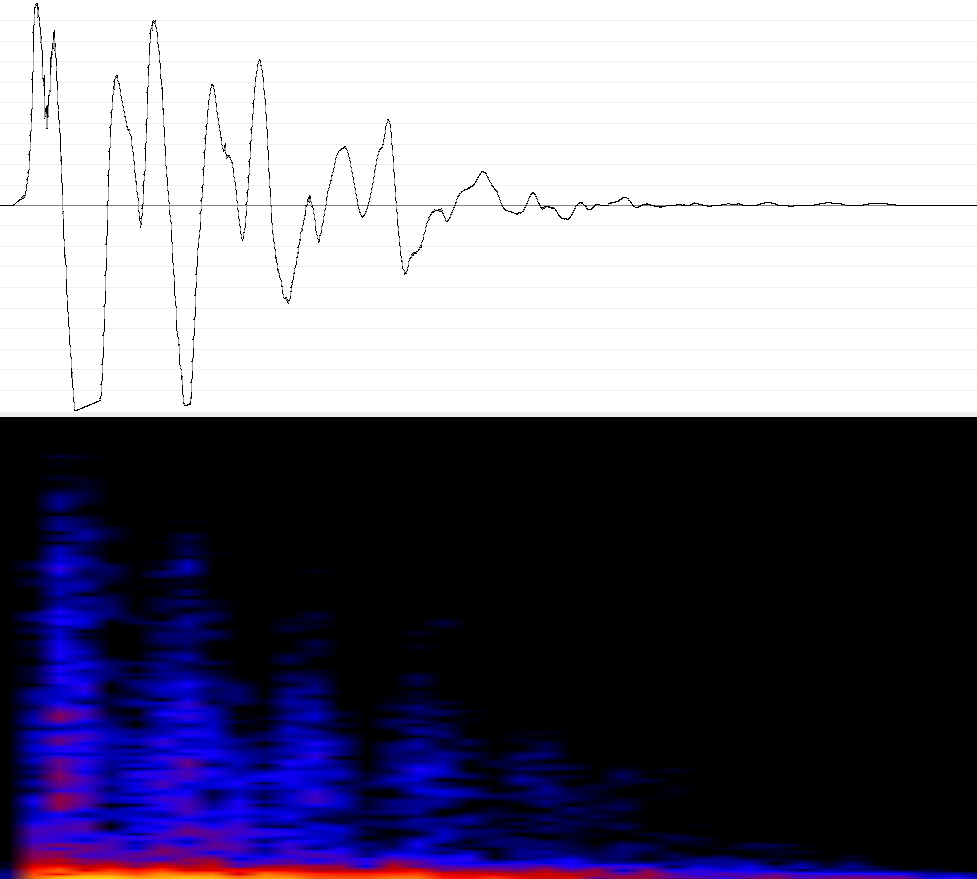
\includegraphics[width=\textwidth]{fig/Kick-wave.png}
		\caption{Kick drum}
		\label{fig:kick-wave}
	\end{subfigure}
	\begin{subfigure}[b]{0.275\textwidth}
		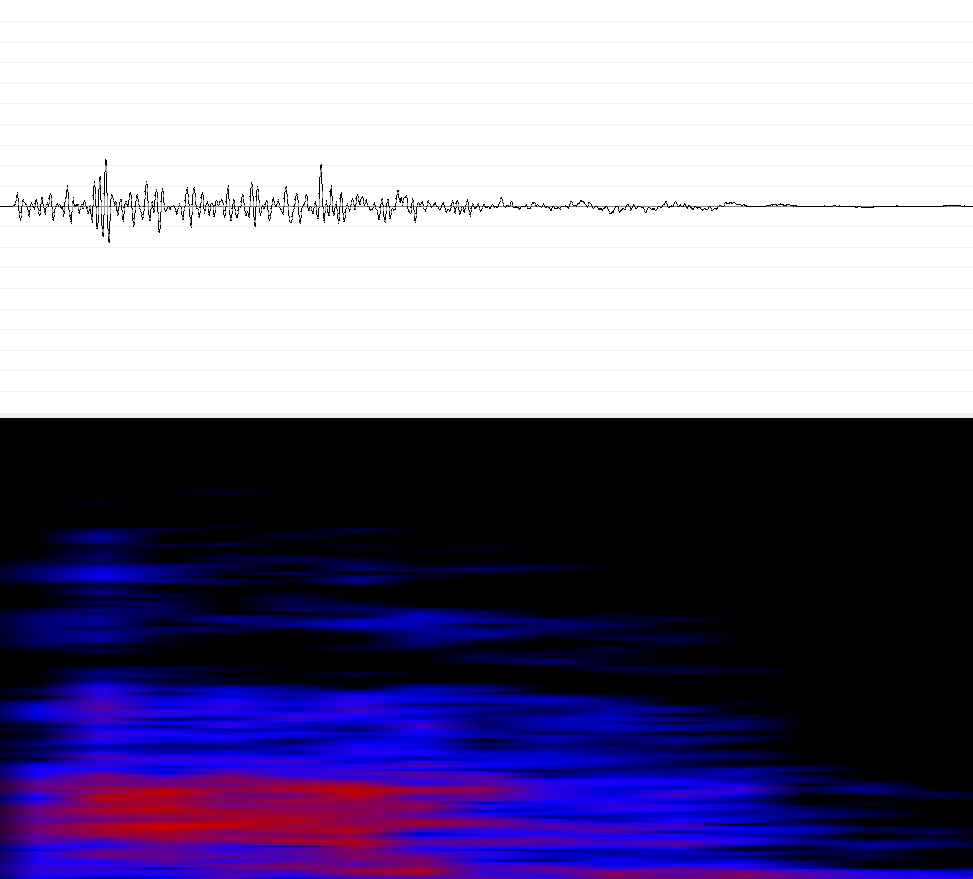
\includegraphics[width=\textwidth]{fig/Snare-wave.png}
		\caption{Snare drum}
		\label{fig:snare-wave}
	\end{subfigure}
	\begin{subfigure}[b]{0.35\textwidth}
		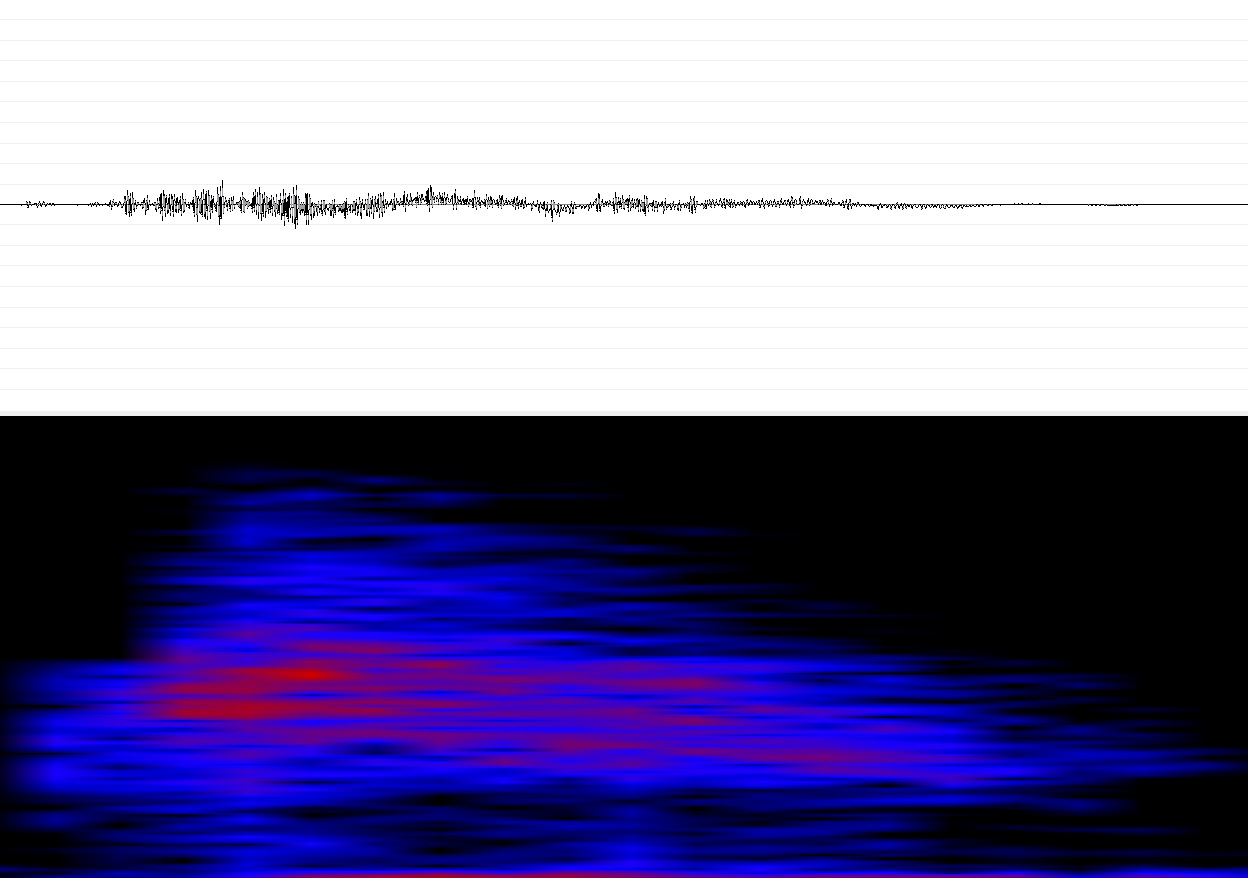
\includegraphics[width=\textwidth]{fig/Hihat-wave.png}
		\caption{Hi-hat}
		\label{fig:hihat-wave}
	\end{subfigure}
	\caption{A presentation of 3 beatboxing sounds' waveform (top) and spectrogram
	\label{fig:chosen-sounds} (bottom).}
\end{figure}

What we can see from these waveforms and spectra is that the kick drum does differ significantly in its frequency content in relation to the snare and hi-hat. The snare and hi-hat does initially seem to have a clear difference in their frequencies, however they do not seem to lie in a very concentrated area of the spectrum, indicating that they might prove difficult to distinct from each other based on the frequency content.
\section{Collection of dataset}
This chapter will go through how a dataset was collected containing only some specific beat boxing sounds.
For collection of the dataset containing beat boxing, only three type of different beat boxing sounds there was made use of a recorder, a microphone, a headset, some boards (to limit the noise from surroundings as much as possible) and a computer to take notes of when the different people did record their beat boxing, The setup of the place where the record took place and be seen on figure \ref{data-collection-pic}. For choosing the people to help us make the beatboxing random convenience method was used. 
\begin{figure}[h]
	\begin{center}
		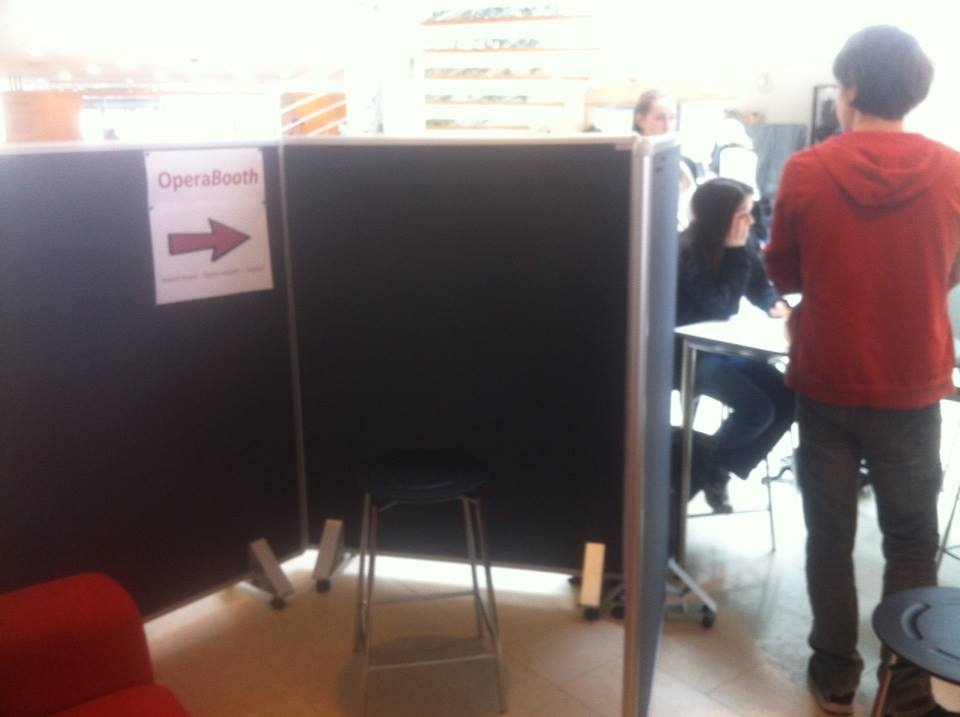
\includegraphics[height=5cm]{fig/dataset_collection.JPG}
		\caption{data-collection-pic}
		\label{data-collection-pic}
	\end{center}
\end{figure}
When the participants sat in the stall they was asked to practice a few different beat boxing sounds, when they had learned one they would be recorded making that  sound this was repeated with three sounds, a kick drum beat boxing sound, a snare drum beat boxing sound and a hi-hat drum beat boxing sound. After they had made the three sounds they were also asked to improvise a short mix of the three beat boxing sounds that they had learned.

\section{Segmentation}
This section will go through how the segmentation of the sound was achieved. The segmentation is needed to locate each sound's endpoints in a signal, i.e. the positions in time at which each sound starts and ends. This is a necessary part of the transcription system as we need to be able to distinct the sounds from each other and not the whole signal as a combination of many sounds.

In this transcription system the segmentation is made by calculating the logarithm of the RMS of each window and if this value, from one window to the next, goes above a threshold it is considered as the starting point of a sound. Similarly when the value falls below the threshold the end of the sound is registered.

The MATLAB function for segmenting the signal analyses the signal using a specified window size and window skip. When all endpoints in the signal are found, a cell array is returned containing the signal divided into segments so that each cell contains the frames for that segment.

\begin{figure}[h]
	\begin{center}
		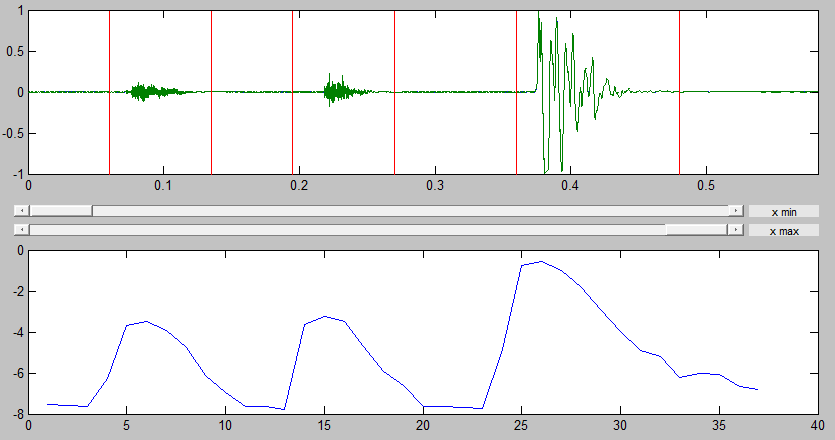
\includegraphics[scale =  0.4]{fig/SegmentationPic.png}
		\caption{An example of how the signal will be segmented. On the top the signal is plotted in the time domain with vertical lines indicating the segmentation points (endpoints). The bottom shows the logarithm of the RMS to the signal from above.}
		\label{SegmentationPic}
	\end{center}
\end{figure}

An example of the result from this segmentation is shown in figure \ref{SegmentationPic}. At the top we see the input signal and vertical lines indicating the endpoints of each segment. On the bottom of the figure a graph of the change in the logarithm of the RMS is plotted where we see a peak at each segment in the signal.
\section{Features}
All feature extraction should be usable independently of each other, thus each calculation of the features is implemented in its own function that will return one or more values about that feature. In the following we have divided the description of the features in 3 categories: the time domain features, spectral domain features and the MFCC in its own category.

% TIME DOMAIN SUBSEC ---- START
\subsection{Time Domain Features}
The time domain features consisting of the Root Mean Square (RMS) and Zero-Crossings (ZC) are implemented as functions that each takes the signal or just a segment as input. The RMS function will return a value indicating what the mean energy of the input is, while the total number of zero-crossings will be returned from the ZC function. Programmatically the implementation is rather simple, as can be seen in figure \ref{snippet-RMS} and \ref{snippet-ZC}, where a single loop iterates through all input samples to calculate the output.

\begin{lstlisting}[caption=Matlab implementation of the RMS algorithm., label=snippet-RMS]
function rms = P4_RMS(x)
    % rms = P4_RMS(x)
    %
    % @param x: signal vector.
    % @retval: returns the root mean square of the signal x.
    rms = 0;
    for ii = 1:length(x)
       rms = rms + x(ii)^2; 
    end
    rms = sqrt(rms / length(x));
end
\end{lstlisting}

\begin{lstlisting}[caption=Matlab implementation of the ZC algorithm., label=snippet-ZC]
function zc = P4_zero_crossing(signal)
    % zc = P4_zero_crossing(x)
    %
    % @param x: signal vector.
    % @retval Returns the total zero crossings of the signal x.
    zc = 0;
    for ii = 2:length(signal)
        if (signal(ii) * signal(ii-1) < 0)
            zc = zc + 1;
        end
    end
end
\end{lstlisting}
% TIME DOMAIN SUBSEC ---- END

% SPECTRAL DOMAIN SUBSEC ---- START
\subsection{Spectral Domain Features}
Spectral domain features uses the information gathered in a spectrogram of the sound. Before being able to actually do any calculations of the spectral features, the spectrogram needs to be produced. Using the built-in function in Matlab for calculating the Fast Fourier Transform (FFT) we can produce a spectrogram of the input sound/segment by looping over the input using the specified window size and skip, see appendix \ref{app:feat-spectrogram}. This spectrogram will then be forwarded to the function corresponding to each of the spectral feature-calculations implemented as follows.

The spectral features implemented are: (a) Centroid, (b) Flux, (c) Rolloff and (d) Skewness, all of which are implemented using the code provided by Alexander Lerch\footnote{\url{http://www.audiocontentanalysis.org/code/}} \citep{ACA}. The extracted value from each of these features is a mean value of the whole signal segment sent into the function. This value is directly used in the classifier to identify and describe that specific segment. See appendices under \ref{app:features} for complete implementation.
% SPECTRAL DOMAIN SUBSEC ---- END

\subsection{Mel Frequency Cepstral Coefficients}
Using the MFCC algorithm provided by Malcolm Slaney we have implemented a version of it that has been adjusted by Bob L. Sturm. This adjustment makes it possible to use different analysis window sizes and skips, please refer to provided Matlab-script "mfcc.m". The algorithm will provide a feature vector with 40 cepstral coefficients that describe every window of the input sound. To use these coefficients, we take a mean over all windows, i.e. for every coefficient we take the mean value of that coefficient over all windows. Out of these 40 mean values, we use the first 20 coefficients.
\\

\colorbox{red}{WE NEED kNN HERE}
\section{Classification using Nearest Neighbour}
This chapter will give information on the classification method called KNN (K nearest neighbour).

Shortly put in \citep{meaningfulNN} the NN is "given a collection of data point and query points in an m-dimentional metric space, find the data point that is closets to the query point".

If going into more detail the above sentence will mean that the NN classification will need a dataset that can train a system \citep{Sinoyr05}, the data used for training has to be notated so that the program that make the classification knows what the different data represent. When one has trained the data they need some value to describe what sound it is  because even though notated they can still be different e.g two people might say a sound different from another, for this one can make use of different features to describe the differences. Then the training data can be see as being scattered out on a field based on what value they gets from the feature. Now when there comes a new input, the input will be given a value from the features. Then based the placement on the field the new data get the program can look at the sounds that are close to it, the inputs sound neighbour. Then with KNN the K will then be how many neighbours that has to be look at before determining what the new input is, then the most represented sound will be chosen as what the input sound is\citep{introKNN}. Another way that one can choose the nearest neighbour is by look at all the neighbour inside some distance (euclidean distance)\citep{NNHD}.

\begin{figure}[h]
	\begin{center}
		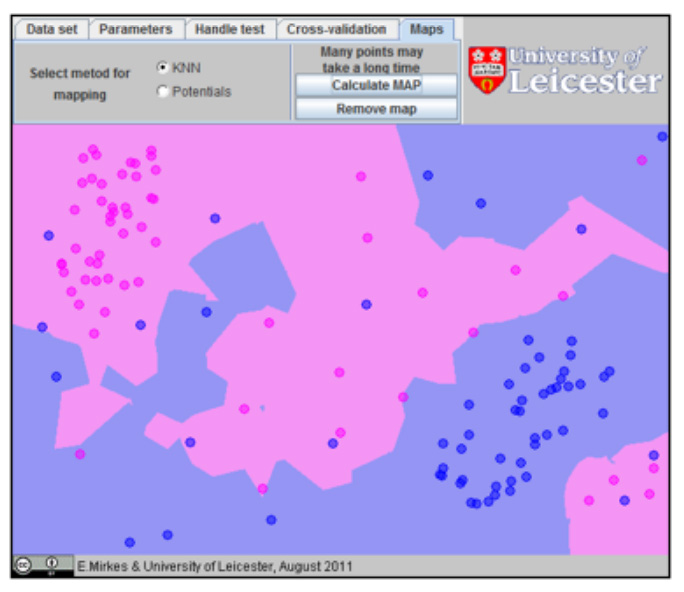
\includegraphics[scale = 0.5]{fig/KNNfig.jpg}
		\caption{KNN field here one can see how the knn will divide the space up with to different classes \citep{introKNN}}
		\label{KNN fig}
	\end{center}
\end{figure}

\colorbox{red}{OUR IMPLEMENTATION WILL BE DESCRIBED HERE (STILL NEEDED!!)}
\section{MATLAB Application}
With all the mathematics behind the whole segmentation, feature extraction and classification parts, we realized that instead of having to manually manage each and every function, a more intuitive way of utilizing the whole setup was needed. This led to the production of a graphical user interface (GUI) consisting of different elements the user can interact with, in order to take a piece of sound, segment it, and then get an automatic classification.

\subsection{Graphical User Interface}
Figure \ref{app-gui} shows the GUI of the active application, in which a waveform has been loaded, segmented, and annotated using the implemented kNN classifier. Starting from the top left corner (rectangle 1), we have a plot of the loaded signal. When this signal has been segmented, either automatically or manually, a set of vertical lines will be plotted to show the segmentation of the waveform. Along with the segmentation, the below plot (rectangle 3) will contain the change in the log-energy ($log(RMS)$), which should show a peak for each segment above. When the segments have been classified, the results will be presented in the table (rectangle 6) with one cell for each segment. To load the unclassified signal into the application the user must choose one of two options: load a sound file or make a new recording. This is done in the top right of the GUI (rectangle 2). Pressing the "Load wave" button will present the user with a file dialog, so a sound file can be located in a directory. The "Start recording" and "Stop recording" buttons will turn on and off the microphone to receive some input. When the sound is loaded a playback button will play the sound for the user. Before the classification, the user must choose the features used in the process. On the middle right side of the GUI (rectangle 4) is where features can be checked and their analysis window size and skip can be adjusted. Finally, below the features (rectangle 5) the user can load a manually segmented (and annotated) dataset for the classifier. Pressing "Load train data" will prompt the user to choose a sound file first, and then a text file containing the segmentation info (such as a segments start-point, duration and annotation). When the features above are chosen and adjusted the classifier can be trained using the "Train" button and finally the signal can be classified from the "Classify" button.

\begin{sidewaysfigure}
\begin{center}
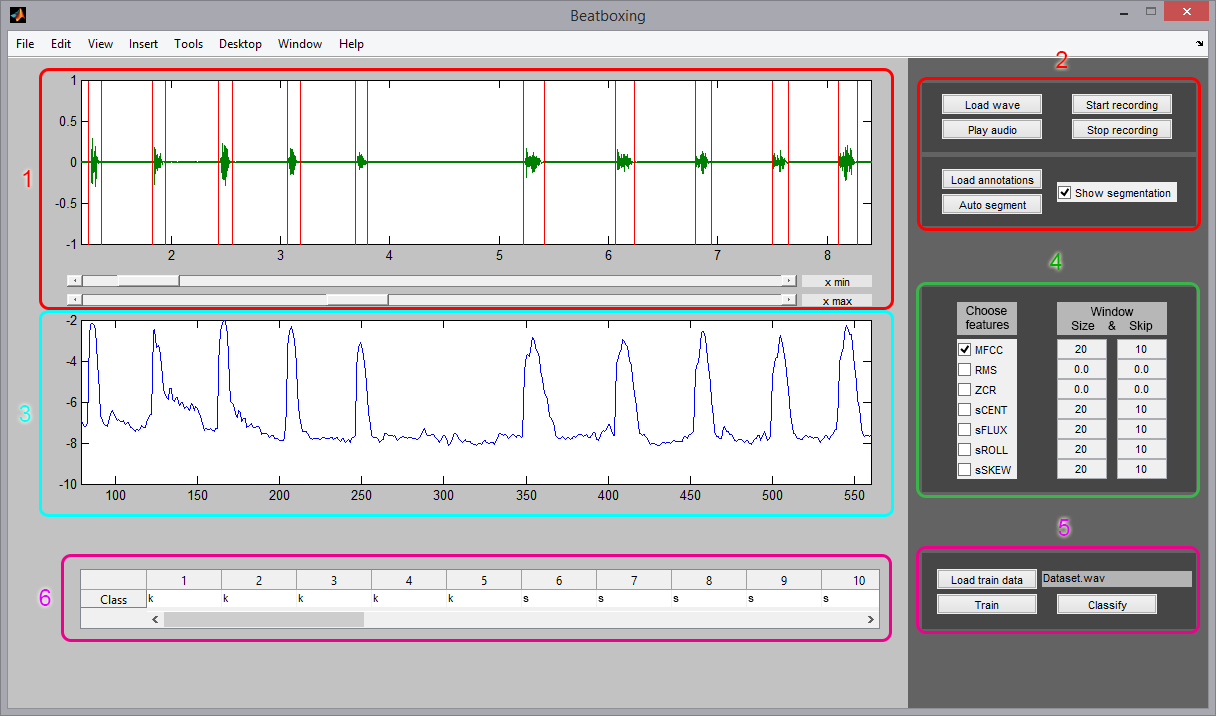
\includegraphics[width=\textwidth]{fig/Application.png}
\caption{Screenshot of the application GUI.}
\label{app-gui}
\end{center}
\end{sidewaysfigure}

\subsection{Application Workflow}
When the user starts the application the flow has to follow a specific path from taking an unclassified signal, segment it, and then automatically classify each sound included. The flow of the application is presented in figure \ref{app-flowchart}. To use the application one has to load a waveform of some recording of a person beatboxing, be it the user or someone else. This waveform then has to be segmented to identify the points at which each beatboxing sound (e.g. a kick drum or hi-hat) starts and ends. This process can either be done manually by the user or it automatically with the built-in segmentation algorithm. The manual process of segmenting the waveform has been explained in section \ref{sec:data-collecting} about data collection using Sonic Visualiser. The automatic segmentation uses the implementation described above.

\begin{figure}
\begin{center}
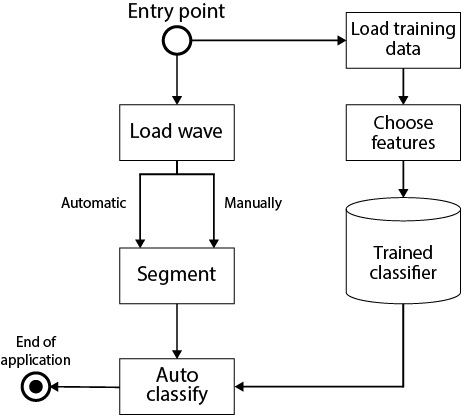
\includegraphics[scale=0.6]{fig/Application_flowchart.png}
\caption{Flowchart of the application.}
\label{app-flowchart}
\end{center}
\end{figure}

Before classifying these segments, the classifier has to be trained. To do this we start by loading a dataset that has been manually segmented. This dataset is a recording of multiple instances of the different beatboxing sounds used for the classification. When this dataset is loaded and segmented, the user must choose which features to use during the classification process. As an example we could choose MFCC using an analysis window size of 16 ms and a window skip of 8 ms. The classifier will then analyse all segments in the training dataset based on their MFCC and then store these analysis results to be used when classifying the unknown waveform.

When the user query a classification of the input waveform the classifier will take each segment from the input and compare it to the stored training data. Each segment will through this process get an annotation, i.e. a classification id, telling the user what kind of sound that segment has been interpreted as. A sequence of these annotation could be: \textit{k k k hh k s}, where the three first segments are classified as kicks followed by a hi-hat and then a snare.

Hereafter the user can adjust chosen features or choose new features to train the classifier again, and/or a new waveform can be loaded into the application and segmented to be classified as well.

\chapter{Evaluation}
\thispagestyle{empty}
% Chapter 'Evaluation'

\section{Methods}
	\subsection{Hypothesis}
		There are many things we could evaluate, as both features, segmentation, and classification are critical parts of the application. Even if only evaluating on the classifier, the number of combinations of features, and parameters of features (window size and window skip), is huge. We want keep a single independent variable. To limit ourselves, we chose not to test any combinations of features, but rather single features one at a time. We will then test that feature for $K \in [1;10]$. We state the null hypothesis that two knn-classifiers with a different k and otherwise identical, will not have result in significantly different confusion tables.
		
		This will be tested for each feature and each feature configuration.
		We will test window sizes of 20ms, 10ms, and 5ms; and we will test window skips of 10ms, 5ms, 2ms respectively. This will be the case for all features using window: MFCC, Spectral Flux, Spectral Centroid, Spectral Skew, and Spectral Rolloff. Only the first 20 MFCC coefficients will be used. RMS and ZCR are calculated over the entire sound.
		
		To determine if the independent variable $k$ has any has any significant effect on resulting confusion tables, the chi squared test is used. Since we are testing over 10 different K, but only on unique combinations of $K_1$ and $K_2$, the amount of tests done in total will be $Tests = 10*9/2 = 45$. We have chosen that the null hypothesis can be disputed, if any calculated probability $p < \alpha$. Further, the Bonferroni correction\citep{bonferroni} will be applied to $\alpha$, such that $\alpha=\alpha/45 = 0.00\overline{1}$.
		
	\subsection{Measures}
		A confusion table is created for each test (each unique combination of variables). This will be shown in percentages (or rather, values between 0 and 1). Overall accuracy is calculated, along with precision, recall, and F-score for each class individually. For the sake of compactness, all the measures are included in an extended confusion table, as shown in the explanatory table \ref{table:eval:explanatory}. 
		The most important measure, for the sake of measuring our transcription system, would be the precision, that is, the amount of correctly transcribed sounds over the actual amount of that sound class.
		Recall should just be ignored, since we only test on the dataset, which means that we always test on all available samples of any given class, meaning that it would be the same as the total amount. This would be different, had the segmentation been part of the evaluation. It is included nonetheless, as further progress with this project might find a need for it. When looking at results, we will judge the performance primarily by accuracy and precision.

			\begin{table}
				\centering
				\begin{tabular}{|c | c | c | c | c |}
					\hline
				 & Real Class(1) & Real Class(2) & Real Class(3) & Precision\\ \hline
					Label(1)  & ... & ... & ... & ...\\ \hline
					Label(2)  & ... & ... & ... & ...\\ \hline
					Label(3) & ... & ... & ... & ...\\ \hline
					F-Score & ... & ... & ... & Accuracy \\ \cline{1-4}
				\end{tabular}
				\caption{$K=1$}
				\label{table:eval:explanatory}
			\end{table}
		
		
	\subsection{Training and Test Sets}
		The dataset consists of sound segments, segmented based on the annotations. This means that our segmentation of sound (present in our application), will not be part of the evaluation.
		The training and test sets of sounds for the KNN classifier are randomly chosen from the same pool (the dataset). It is distributed between the training and test set in a 70\%/30\% ratio, accordingly, for each class. This means there will not be a fixed number of sounds for each class (neither total nor divided), but rather a fixed distribution between the number of training and test sounds for each class. We can do this instead of e.g. k-fold cross validation, due to scale of our collected dataset. The ratio was suggested by our supervisor\footnote{Bob L. Sturm}. The composition of the entire dataset has been summarized in table \ref{table:eval:datasetComposition}. 
		Furthermore, all sounds with a duration less than the windowsize used for feature calculation, are removed before testing. This is done before splitting the dataset, such as to make sure we do not distort the 70/30 distribution.

		\begin{table}
			\centering
			\begin{tabular}{|l|r|r|}
					\hline
					Value  &  Count  & Percent \\ \hline
			      noise    &  150    & 10.19\% \\ \hline
			          k    &  466    & 31.66\% \\ \hline
			  undefined    &  130    &  8.83\% \\ \hline
			          s    &  331    & 22.49\% \\ \hline
			         hh    &  395    & 26.83\% \\ \hline
			      TOTAL    &  1472	 & 100.00\% \\ \hline

			\end{tabular}
			\caption{Dataset composition}
			\label{table:eval:datasetComposition}
		\end{table}
		
		
	\subsection{Test Implementation}		% REFERENCES TO APPENDIX!
		To ease the testing of the transcription system, some additional scripts were created: \texttt{prettyPrintTables.m}, \texttt{testPlots.m}, \texttt{printDataStats.m}, and \texttt{DoEverything.m}.
		The \texttt{printPrettyTables.m} script simply runs a test and formats the results in tables usable for \LaTeX, while \texttt{testPlots.m} creates plots for precision, recall, and F over K, including the overall accuracy in all three plots, and saves them as PNG images\footnote{\url{using: https://github.com/ojwoodford/export\_fig}}. They will not be described further, as they have no real functional effect on the system -  they are just helping facilitating the tests. These scripts are quite simple and well-commented, and thus should require no more than than a simple mention, as they do not include features, not already explained in chapter \ref{chapter:OurApproach}.
		All code can be found in the digital appendix.
			
 
\section{Results}
	
	For all results found, some interpretation of the data and statistics will be presented, although it will be kept short due to the breadth of configurations tested. Further discussion about the relevance of the data, possible mistakes that affected results, or similar, will be covered in chapter \ref{chapter:Discussion}. Only the relevant results will be shown and discussed, based on the accuracy, however the other measures will be considered as well. All data can be found in appendix \ref{app:res}. 

	%
	% RMS
	%
	
	\subsection{Root Mean Square}

	
		The best results using the RMS feature vector was observed using $K=9$ with accuracy 61.5\% (see appendixx \ref{app:RMS:9:best}). Some configurations had slightly higher precision in classes 's' and 'hh', although this seems minimal (see e.g. appendix  \ref{app:rms:k6} and \ref{app:rms:k8}). The worst observed was using $K=1$, with accuracy 53.9\% see appendix \ref{app:RMS:1:worst}. All results from for the RMS feature can be found in appendix \ref{app:res:rms}. The $X^2$ test revealed no significant differences between any two $K$ (see all p in \ref{xlrms11}).

		
	%
	%	ZCR
	%
	
	\subsection{Zero Crossing Rate}
%		\begin{figure}
%			\centering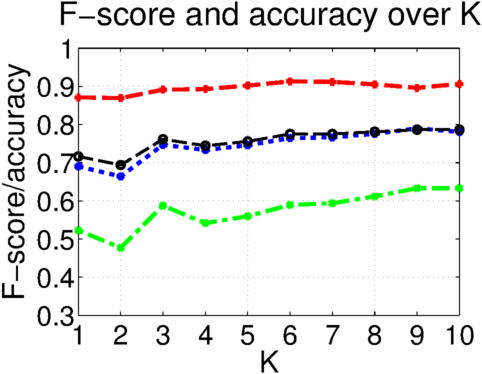
\includegraphics[width=0.3\textwidth]{tex/appendices/test/zcr11FP.png}
%			\centering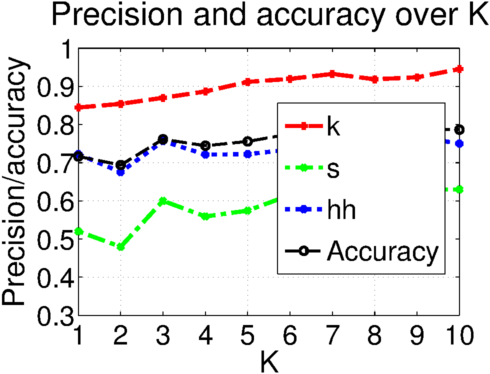
\includegraphics[width=0.3\textwidth]{tex/appendices/test/zcr11_P.png}
%			\centering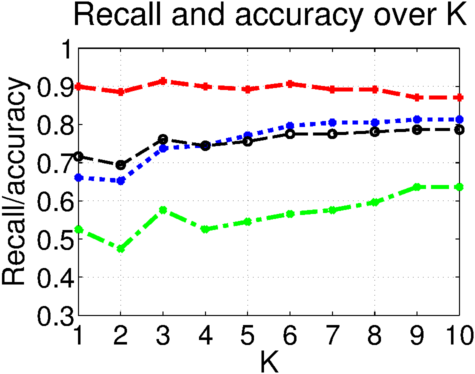
\includegraphics[width=0.3\textwidth]{tex/appendices/test/zcr11_R.png}
%			\label{fig:eval:zcr}
%			\caption{Plots over K for Zero Crossing Rate}
%		\end{figure}
%		
%		\begin{table}
%			\begin{subtable}[tbp]{0.45\textwidth}
%				\centering
%				\begin{tabular}{|c|c|c|c"c|}
%					\cline{2-5}
%					 \multicolumn{1}{c|}{} & \textbf{k}  & \textbf{s}  & \textbf{hh}  & Prec.\\ \hline
%					 \textbf{k} & \textcolor{red}{0.871} & 0.081 & 0.017 & 0.924\\ \hline
%					 \textbf{s} & 0.122 & \textcolor{red}{0.636} & 0.169 & 0.630\\ \hline
%					 \textbf{hh} & 0.122 & 0.283 & \textcolor{red}{0.814} & 0.768\\ \Xhline{2\arrayrulewidth}
%					 F & 0.896 & 0.633 & 0.790 & \textcolor{blue}{0.787}\\ \hline
%				\end{tabular}
%				\label{table:eval:zcrBest1}
%				\caption{$K=9$ (Best)}
%			\end{subtable}
%		
%			\begin{subtable}[tbp]{0.45\textwidth}
%				\centering
%				\begin{tabular}{|c|c|c|c"c|}
%					\cline{2-5}
%					 \multicolumn{1}{c|}{} & \textbf{k}  & \textbf{s}  & \textbf{hh}  & Prec.\\ \hline
%					 \textbf{k} & \textcolor{red}{0.871} & 0.051 & 0.017 & 0.945\\ \hline
%					 \textbf{s} & 0.122 & \textcolor{red}{0.636} & 0.169 & 0.630\\ \hline
%					 \textbf{hh} & 0.122 & 0.313 & \textcolor{red}{0.814} & 0.750\\ \Xhline{2\arrayrulewidth}
%					 F & 0.906 & 0.633 & 0.780 & \textcolor{blue}{0.787}\\ \hline
%				\end{tabular}
%				\label{table:eval:zcrBest2}
%				\caption{$K=10$ (Best)}
%			\end{subtable}
%			
%			\begin{subtable}[tbp]{0.45\textwidth}
%				\centering
%				\begin{tabular}{|c|c|c|c"c|}
%					\cline{2-5}
%					 \multicolumn{1}{c|}{} & \textbf{k}  & \textbf{s}  & \textbf{hh}  & Prec.\\ \hline
%					 \textbf{k} & \textcolor{red}{0.885} & 0.162 & 0.042 & 0.854\\ \hline
%					 \textbf{s} & 0.108 & \textcolor{red}{0.475} & 0.305 & 0.480\\ \hline
%					 \textbf{hh} & 0.108 & 0.364 & \textcolor{red}{0.653} & 0.675\\ \Xhline{2\arrayrulewidth}
%					 F & 0.869 & 0.477 & 0.664 & \textcolor{blue}{0.694}\\ \hline
%				\end{tabular}
%				\label{table:eval:zcrWorst}
%				\caption{$K=2$ (Worst)}
%			\end{subtable}
%			
%			\caption{Measures over K using ZCR}
%		\end{table}
		

		The best results using ZCR was a tie between $K=9$ (appendix \ref{app:zcr:best}) and $k=10$ (appendix \ref{app:zcr:best2}), both with accuracy 78.7\%. In the results from $K=9$, the precision of the hh is slightly better than in $K=10$ (75\% vs 67.5\%). In $K=10$, the precision of the kick is slightly better (94.6\% vs 92.4\%). The worst results was observed with $K=2$, having accuracy 69.4\%(appendix \ref{app-ZCR-Worst}). No tests were deemed significant by $X^2$ testing. See all $X^2$ results in appendix \ref{app:res:zcr};
		
	%	
	%	MFCC
	%	
		
	\subsection{Mel Frequency Cepstrum Coefficients}
%		\begin{figure}
%			\centering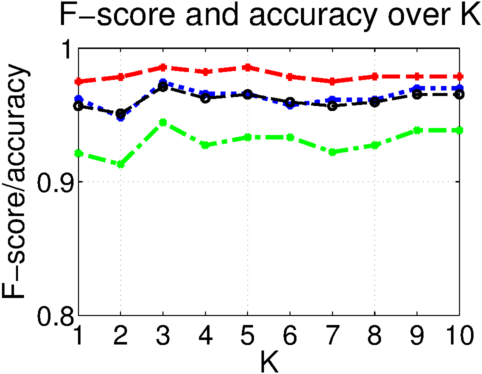
\includegraphics[width=0.3\textwidth]{tex/appendices/test/mfcc2010FP.png}
%			\centering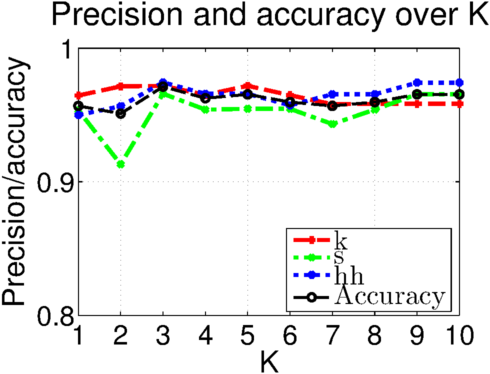
\includegraphics[width=0.3\textwidth]{tex/appendices/test/mfcc2010_P.png}
%			\centering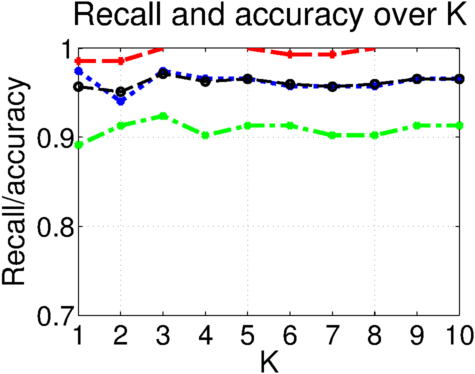
\includegraphics[width=0.3\textwidth]{tex/appendices/test/mfcc2010_R.png}
%			
%			\caption{Plots over K for MFCC with 20ms windows and 10ms window skips}
%		\end{figure}
%		\begin{figure}
%			\centering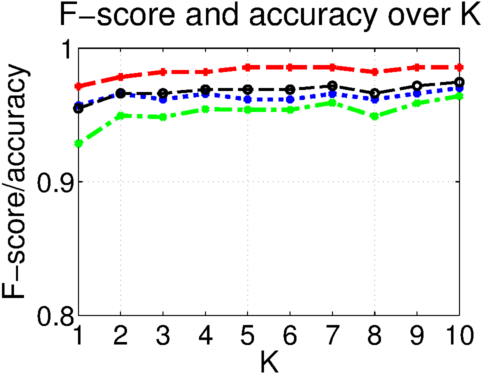
\includegraphics[width=0.3\textwidth]{tex/appendices/test/mfcc105FP.png}
%			\centering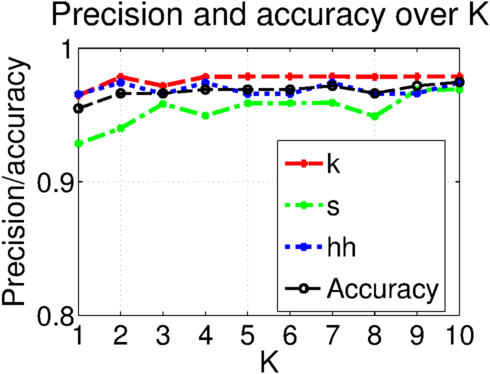
\includegraphics[width=0.3\textwidth]{tex/appendices/test/mfcc105_P.png}
%			\centering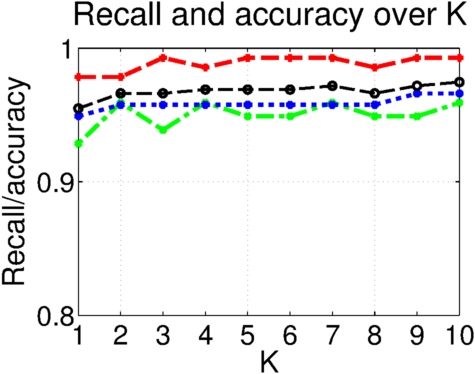
\includegraphics[width=0.3\textwidth]{tex/appendices/test/mfcc105_R.png}
%			
%			\caption{Plots over K for MFCC with 10ms windows and 5ms window skips}
%		\end{figure}
%		\begin{figure}
%			\centering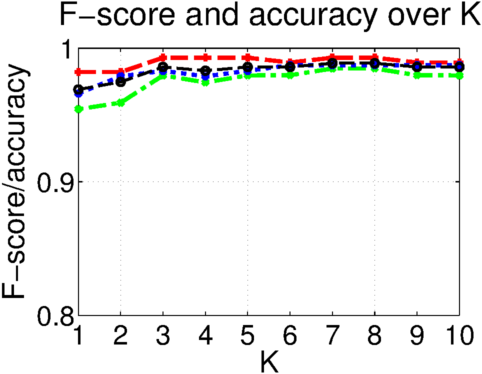
\includegraphics[width=0.3\textwidth]{tex/appendices/test/mfcc52FP.png}
%			\centering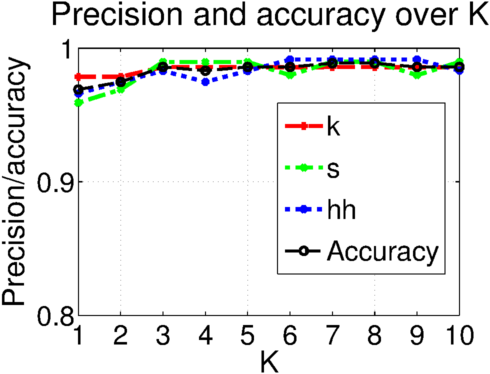
\includegraphics[width=0.3\textwidth]{tex/appendices/test/mfcc52_P.png}
%			\centering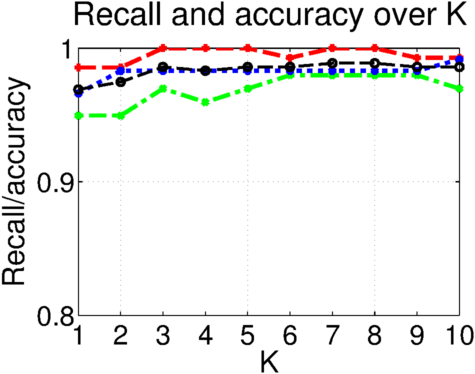
\includegraphics[width=0.3\textwidth]{tex/appendices/test/mfcc52_R.png}
%			
%			\caption{Plots over K for MFCC with 5ms windows and 2ms window skips}
%		\end{figure}\clearpage
%		
%		\begin{table}
%			\begin{subtable}[tbp]{0.45\textwidth}
%				\centering
%				\begin{tabular}{|c|c|c|c"c|}
%					\cline{2-5}
%					 \multicolumn{1}{c|}{} & \textbf{k}  & \textbf{s}  & \textbf{hh}  & Prec.\\ \hline
%					 \textbf{k} & \textcolor{red}{1.000} & 0.010 & 0.008 & 0.986\\ \hline
%					 \textbf{s} & 0.000 & \textcolor{red}{0.980} & 0.008 & 0.990\\ \hline
%					 \textbf{hh} & 0.000 & 0.010 & \textcolor{red}{0.983} & 0.991\\ \Xhline{2\arrayrulewidth}
%					 F & 0.993 & 0.985 & 0.987 & \textcolor{blue}{0.989}\\ \hline
%				\end{tabular}
%				\caption{$wSize=5ms, wSkip=2ms, K=7$}
%				\label{table:eval:mfccBest1}
%			\end{subtable}
%			\hfill
%			\begin{subtable}[tbp]{0.45\textwidth}
%				\centering
%				\begin{tabular}{|c|c|c|c"c|}
%					\cline{2-5}
%					 \multicolumn{1}{c|}{} & \textbf{k}  & \textbf{s}  & \textbf{hh}  & Prec.\\ \hline
%					 \textbf{k} & \textcolor{red}{1.000} & 0.010 & 0.008 & 0.986\\ \hline
%					 \textbf{s} & 0.000 & \textcolor{red}{0.980} & 0.008 & 0.990\\ \hline
%					 \textbf{hh} & 0.000 & 0.010 & \textcolor{red}{0.983} & 0.991\\ \Xhline{2\arrayrulewidth}
%					 F & 0.993 & 0.985 & 0.987 & \textcolor{blue}{0.989}\\ \hline
%				\end{tabular}
%				\caption{$wSize=5ms, wSkip=2ms, K=8$}
%				\label{table:eval:mfccBest2}
%			\end{subtable}
%			\hfill
%			\begin{subtable}[tbp]{0.45\textwidth}
%			\centering
%			\begin{tabular}{|c|c|c|c"c|}
%			\cline{2-5}
%			 \multicolumn{1}{c|}{} & \textbf{k}  & \textbf{s}  & \textbf{hh}  & Prec.\\ \hline
%			 \textbf{k} & \textcolor{red}{0.986} & 0.043 & 0.000 & 0.971\\ \hline
%			 \textbf{s} & 0.007 & \textcolor{red}{0.913} & 0.060 & 0.913\\ \hline
%			 \textbf{hh} & 0.007 & 0.043 & \textcolor{red}{0.940} & 0.957\\ \Xhline{2\arrayrulewidth}
%			 F & 0.978 & 0.913 & 0.948 & \textcolor{blue}{0.951}\\ \hline
%			\end{tabular}
%			\caption{$wSize=20ms, wSkip=10ms, K=2$}
%			\label{table:eval:mfccWorst}
%			\end{subtable}
%			
%			\caption{Measures over K using MFCC}
%		\end{table}
		

		Over all three configurations of the MFCC feature vector, the best performing were $K=7$ and $K=8$ with accuracies 98.9\%, when using a window size of 5ms and skip of 2ms (see appendix \ref{app:MFCC:7:best} and \ref{app:MFCC:8:best}). Some of the other results with the same parameters reach similar performance in regards to precision per class (see appendix \ref{tlmfcc52}). The worst performing, with 95.1\% accuracy, is using 20ms window size and 10ms skip with $K=2$ (see appendixs \ref{app:Mfcc:2:worst}). It still has better precision for kick than some others(e.g. $K=4$ or $K=6$), but some have similar hh precision (e.g. $K=1$ or $K=6$). No $X^2$ results were considered significant (although some came quite close; see appendix \ref{xlmfcc52}).
		
	%
	% SC
	%
	\subsection{Spectral Centroid}

		Using the Spectral Centroid feature, the best configuration found, with accuracy 82.8\% was 10ms windows and 5ms window skips, and $K=9$, as shown in appendix \ref{app:sc:9:best}. Some results show similar or better precision in some classes, e.g. $K=8$. The worst accuracy seen, was usisng 20ms window size, 10ms window skip, and $K=2$, with accuracy 73.8\%, as shown in table \ref{app:SC:2:worst}. $X^2$-test revealed no significant differences (see all in appendix \ref{app:res:sc}).
		
				
	% 
	% SS
	%
	\subsection{Spectral Skew}
			
%		\begin{figure}
%			\centering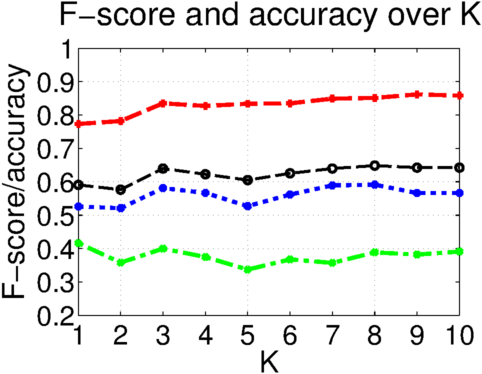
\includegraphics[width=0.3\textwidth]{tex/appendices/test/sskew2010FP.png}
%			\centering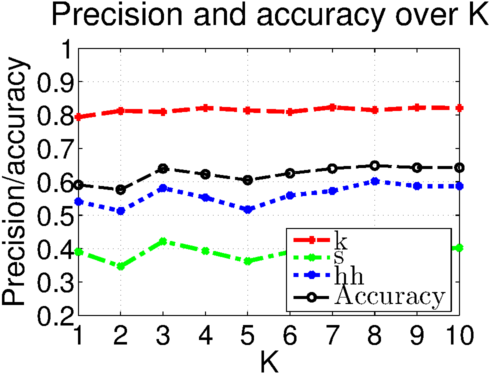
\includegraphics[width=0.3\textwidth]{tex/appendices/test/sskew2010_P.png}
%			\centering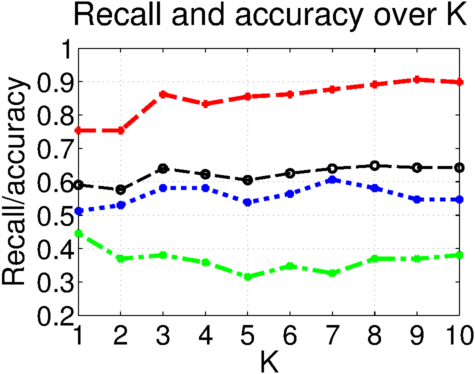
\includegraphics[width=0.3\textwidth]{tex/appendices/test/sskew2010_R.png}
%			
%			\caption{Plots over K for Spectral Skew with 20ms windows and 10ms window skips}
%		\end{figure}
%		
%		\begin{figure}
%			\centering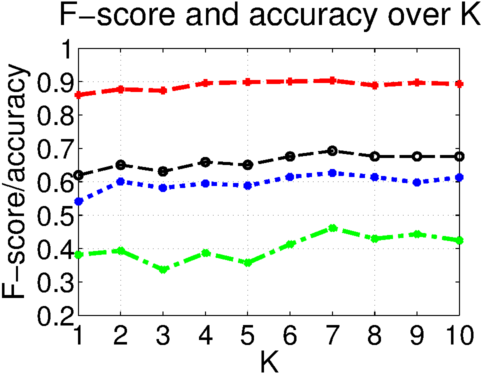
\includegraphics[width=0.3\textwidth]{tex/appendices/test/sskew105FP.png}
%			\centering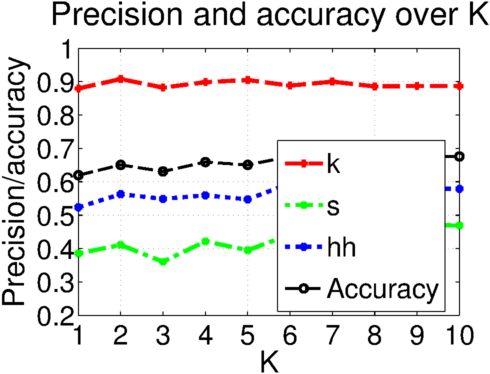
\includegraphics[width=0.3\textwidth]{tex/appendices/test/sskew105_P.png}
%			\centering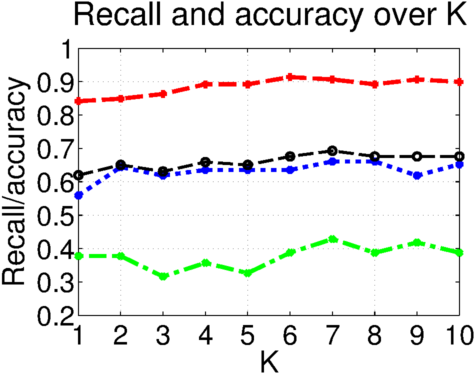
\includegraphics[width=0.3\textwidth]{tex/appendices/test/sskew105_R.png}
%				
%				\caption{Plots over K for Spectral Skew with 10ms windows and 5ms window skips}
%		\end{figure}
%		\begin{figure}
%			\centering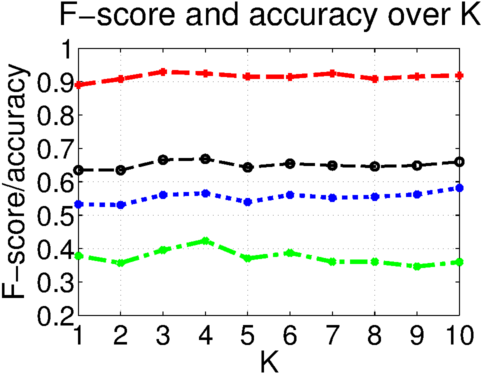
\includegraphics[width=0.3\textwidth]{tex/appendices/test/sskew52FP.png}
%			\centering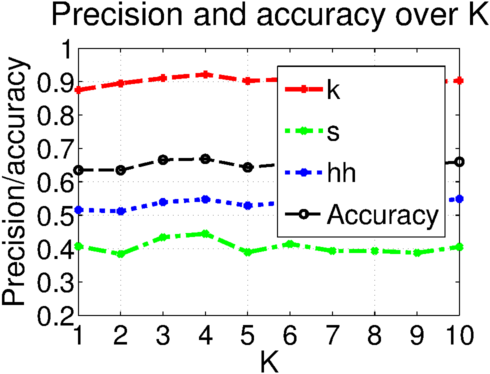
\includegraphics[width=0.3\textwidth]{tex/appendices/test/sskew52_P.png}
%			\centering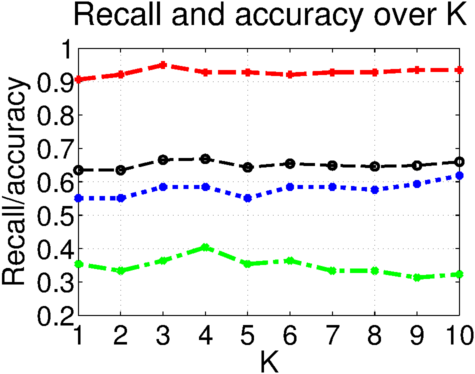
\includegraphics[width=0.3\textwidth]{tex/appendices/test/sskew52_R.png}
%				
%				\caption{Plots over K for Spectral Skew with 5ms windows and 2ms window skips}
%		\end{figure}\clearpage
%		
%		\begin{table}
%			\begin{subtable}[h]{0.45\textwidth}
%				\centering
%				\begin{tabular}{|c|c|c|c"c|}
%					 \cline{2-5}
%					 \multicolumn{1}{c|}{} & \textbf{k}  & \textbf{s}  & \textbf{hh}  & Prec.\\ \hline
%					 \textbf{k} & \textcolor{red}{0.942} & 0.031 & 0.008 & 0.970\\ \hline
%					 \textbf{s} & 0.058 & \textcolor{red}{0.786} & 0.288 & 0.647\\ \hline
%					 \textbf{hh} & 0.058 & 0.184 & \textcolor{red}{0.703} & 0.822\\ \Xhline{2\arrayrulewidth}
%					  F & 0.956 & 0.710 & 0.758 & \textcolor{blue}{0.820}\\ \hline
%				\end{tabular}
%				\caption{$wSize=10ms, wSkip=5ms, K=7$}
%				\label{table:eval:skewBest}
%			\end{subtable}
%			\hfill
%			\begin{subtable}[h]{0.45\textwidth}
%				\centering
%				\begin{tabular}{|c|c|c|c"c|}
%					\cline{2-5}
%					 \multicolumn{1}{c|}{} & \textbf{k}  & \textbf{s}  & \textbf{hh}  & Prec.\\ \hline
%					 \textbf{k} & \textcolor{red}{0.964} & 0.081 & 0.008 & 0.937\\ \hline
%					 \textbf{s} & 0.036 & \textcolor{red}{0.768} & 0.280 & 0.667\\ \hline
%					 \textbf{hh} & 0.036 & 0.152 & \textcolor{red}{0.712} & 0.848\\ \Xhline{2\arrayrulewidth}
%					 F & 0.950 & 0.714 & 0.774 & \textcolor{blue}{0.826}\\ \hline
%				\end{tabular}
%				\caption{$wSize=5ms, wSkip=2ms, K=7$}
%				\label{table:eval:skewKicker}
%			\end{subtable}
%			\hfill
%			\begin{subtable}[h]{0.45\textwidth}
%				\centering
%				\begin{tabular}{|c|c|c|c"c|}
%					\cline{2-5}
%					 \multicolumn{1}{c|}{} & \textbf{k}  & \textbf{s}  & \textbf{hh}  & Prec.\\ \hline
%					 \textbf{k} & \textcolor{red}{0.920} & 0.163 & 0.009 & 0.888\\ \hline
%					 \textbf{s} & 0.072 & \textcolor{red}{0.446} & 0.239 & 0.519\\ \hline
%					 \textbf{hh} & 0.072 & 0.391 & \textcolor{red}{0.752} & 0.704\\ \Xhline{2\arrayrulewidth}
%					 F & 0.904 & 0.480 & 0.727 & \textcolor{blue}{0.738}\\ \hline
%				\end{tabular}
%				\caption{$wSize=20ms, wSkip=10ms, K=2$}
%				\label{table:eval:skewWorst}
%			\end{subtable}
%			\caption{Measures over K using Spectral Skewness}
%		\end{table}
		

		The most accurate result using Spectral Skew was 82\%, was $K=7$ with 10ms window size and 5ms window skip, as shown in appendix \ref{app:SS:7:best}. Some other tests was more precise on kicks (e.g. Spectral Skew with 5ms window and 2ms window skip, with $K=7$, see \ref{app:SS:7:kickbest}). The least accurate result was $K=2$, using 20ms window size, 10ms window skip (see appendix \ref{app:SS:2:worst}). $X^2$-test did not show any significant results.
	
	%
	% SF
	%
	\subsection{Spectral Flux}
		
%		\begin{figure}
%		
%			\label{figJitter}
%			\centering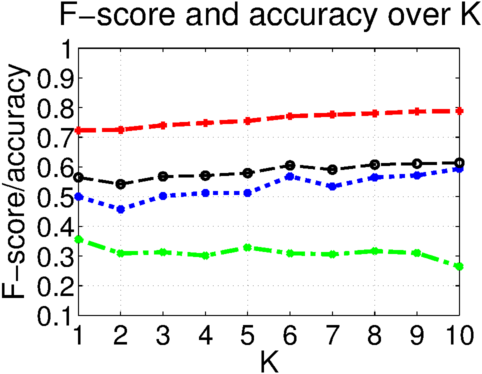
\includegraphics[width=0.3\textwidth]{tex/appendices/test/sflux2010FP.png}
%			\centering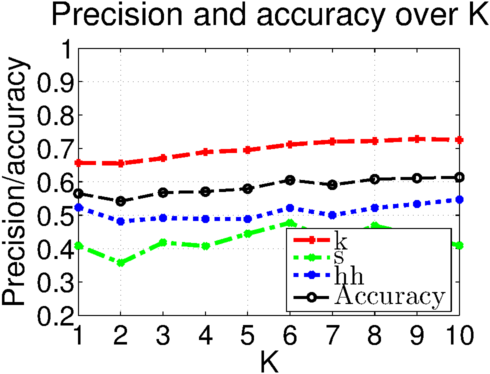
\includegraphics[width=0.3\textwidth]{tex/appendices/test/sflux2010_P.png}
%			\centering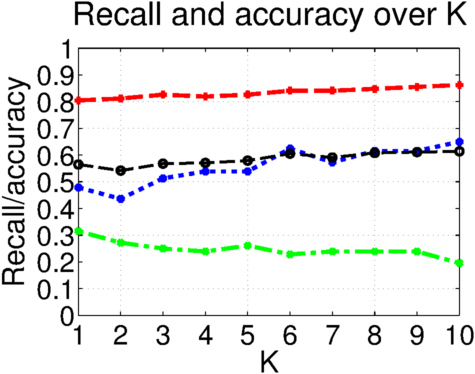
\includegraphics[width=0.3\textwidth]{tex/appendices/test/sflux2010_R.png}
%			
%			\caption{Plots over K for Spectral Flux with 20ms windows and 10ms window skips}
%		\end{figure}
%		\begin{figure}
%		
%		
%			\centering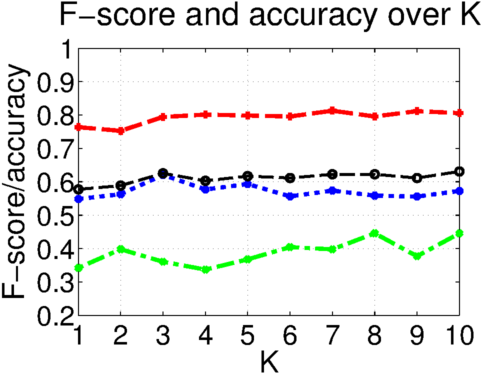
\includegraphics[width=0.3\textwidth]{tex/appendices/test/sflux105FP.png}
%			\centering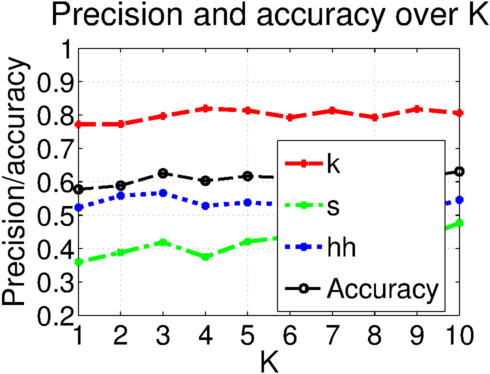
\includegraphics[width=0.3\textwidth]{tex/appendices/test/sflux105_P.png}
%			\centering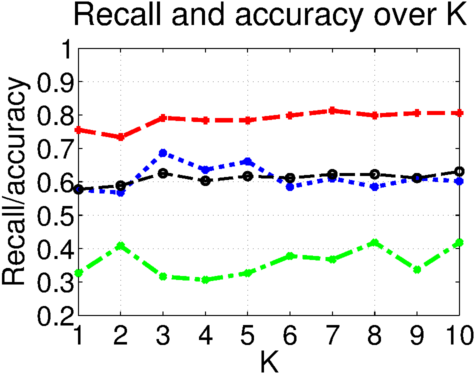
\includegraphics[width=0.3\textwidth]{tex/appendices/test/sflux105_R.png}
%				
%				\caption{Plots over K for Spectral Flux with 10ms windows and 5ms window skips}
%		\end{figure}
%		\begin{figure}
%		
%		
%			\centering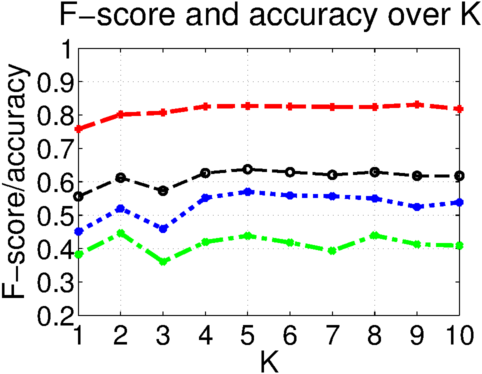
\includegraphics[width=0.3\textwidth]{tex/appendices/test/sflux52FP.png}
%			\centering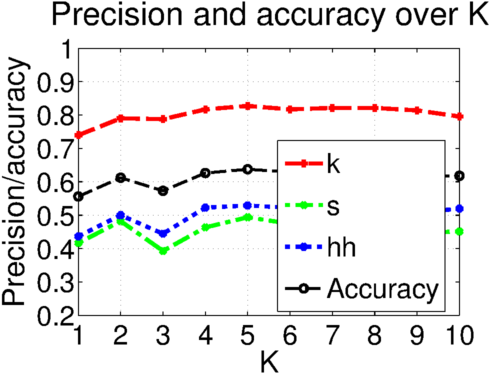
\includegraphics[width=0.3\textwidth]{tex/appendices/test/sflux52_P.png}
%			\centering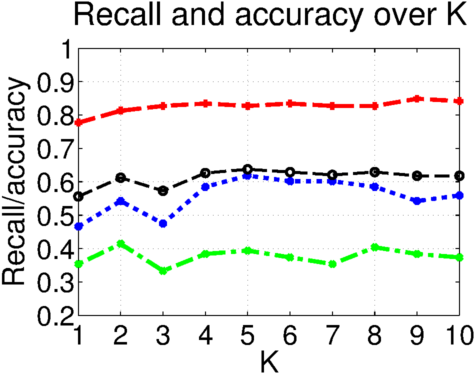
\includegraphics[width=0.3\textwidth]{tex/appendices/test/sflux52_R.png}
%				
%				\caption{Plots over K for Spectral Flux with 5ms windows and 2ms window skips}
%		\end{figure}
%		
%		\begin{table}
%			\begin{subtable}[h]{0.45\textwidth}
%				\centering
%				\begin{tabular}{|c|c|c|c"c|}
%					\cline{2-5}
%					 \multicolumn{1}{c|}{} & \textbf{k}  & \textbf{s}  & \textbf{hh}  & Prec.\\ \hline
%					 \textbf{k} & \textcolor{red}{0.827} & 0.121 & 0.102 & 0.827\\ \hline
%					 \textbf{s} & 0.050 & \textcolor{red}{0.394} & 0.280 & 0.494\\ \hline
%					 \textbf{hh} & 0.050 & 0.485 & \textcolor{red}{0.619} & 0.529\\ \Xhline{2\arrayrulewidth}
%					 F & 0.827 & 0.438 & 0.570 & \textcolor{blue}{0.638}\\ \hline
%				\end{tabular}
%				\caption{$wSize=5ms, wSkip=2ms, K=5$}
%				\label{table:eval:fluxBest}
%			\end{subtable}
%			\hfill
%			\begin{subtable}[h]{0.45\textwidth}
%				\centering
%				\begin{tabular}{|c|c|c|c"c|}
%					\cline{2-5}
%					 \multicolumn{1}{c|}{} & \textbf{k}  & \textbf{s}  & \textbf{hh}  & Prec.\\ \hline
%					 \textbf{k} & \textcolor{red}{0.812} & 0.293 & 0.274 & 0.655\\ \hline
%					 \textbf{s} & 0.080 & \textcolor{red}{0.272} & 0.291 & 0.357\\ \hline
%					 \textbf{hh} & 0.080 & 0.435 & \textcolor{red}{0.436} & 0.481\\ \Xhline{2\arrayrulewidth}
%					 F & 0.725 & 0.309 & 0.457 & \textcolor{blue}{0.542}\\ \hline
%				\end{tabular}
%				\caption{$wSize=20ms, wSkip=10ms, K=2$}
%				\label{table:eval:fluxWorst}
%			\end{subtable}
%			
%			\caption{Measures over K using Spectral Flux}
%		\end{table}
		
		The most accurate results with the Spectral Flux feature vector, was with 5ms window size, 2ms window skip, and $K=5$ (appendix \ref{app:SF:5:best}), however several test configurations using other feature parameters, show better precision for the highhat. The worst in terms of accuracy is the Spectral Flux using 20ms windows and 10ms window skips, with $K=2$, see appendix \ref{app:SF:2:worst}.	$X^2$ showed no significant results.


\chapter{Discussion}
\label{chapter:Discussion}
\thispagestyle{empty}
\paragraph{Test results} \hspace{0pt} \\
To recap slightly from the previous chapter: Overall, the highest accuracy was obtained using MFCC over a window of 5ms with a skip of 2ms, with $k=7$ and $k=8$. Our $X^2$ tests did not show a significant difference even once, so our null-hypothesis stands true. This was unexpected, although some probabilities come very close, so perhaps the result might look different in future tests. Alternatively one could use a different test, for example a t-test over precision.

Some interesting points were found in many tests with $k$ between 1 and 5, namely the jumps in measures (y) can be seen in several plots, e.g. \ref{cmon}. We attributed this to even and uneven numbers, as they could shift the decision between classes, or even result in a random decision if e.g. the two nearest neighbours are of different classes.

In general a higher $k$ meant better performance, although on some plots, the measures\footnote{Precision, Recall, Accuracy, F} seem to begin a descent when $k$ approaches 10. This makes us think that it would be worth testing even greater ranges of $k$. 
Furthermore, we generally see that smaller window sizes (and corresponding skips) yields better performance. This make sense, since more data gives higher acuity. It is, however, a trade-off between complexity and performance - something to take into consideration for future prospect

We were surprised by the results of the spectral features, as they showed poor to mediocre results. This was quite the opposite to the expected outcome; an expectation we based on the proposed effectiveness of some of these on beatboxing sounds \citep{Sinyor05}. There is a likelihood that the fault is ours, though, as we could have produced faulty code, as a result of limited MATLAB scripting skills. Too little test-data could also have affected our outcome\footnote{according to our supervisor, Bob. L. Sturm}.

% Direct errors we could have cause

\paragraph{Bias} \hspace{0pt} \\
% random division of dataset
To decrease the probability of obtaining bias, we have been careful to only have one independent variable i.e. variations in $k$, thus we are sure that the measured statistical probability given a 1\% level of significance is sufficient to estimate the preferred value of $k$. However, we can in by no means reject that other factors might have contaminated the test data. Possible bias could e.g. be the k-NN accidentally picking a wrong class. The statistical uncertainty will naturally be reduced the more time the test program is run; hence we can assume that the hypothesis will be further substantiated upon evaluating the other factors of the program independently.\\


\paragraph{Future Prospects} \hspace{0pt}
To expand on the transcription part of our system a possibility could be to synthesize an output instead of a text note. This synthesis could generate a sound representing the sound input by the user, to imitate a musical instrument, e.g. a real kick-drum or hi-hat.

Another way of synthesizing an output could be to use a system like earGram in conjunction with our classification\footnote{Homepage for the earGram application: \url{https://sites.google.com/site/eargram/}}. This would make it possible to input a beatboxing sound and then, through concatenative synthesis in earGram, an output sound. Through this concatenative synthesis, the input sound would undergo an analysis to find sound snippets from a database that sound similar to each piece of the input. The output could then sound like real instruments if the database consisted of recordings of real instruments.

Right now only three beatboxing sounds can, to some extend, be classified limiting the user to only be able to use kicks, snares, and hi-hat sounds. If further development on the system should occur, an expansion on the classifiable sounds would be a suitable subject as it would open up for a broader spectrum of sounds/beats to be transcribed.

Another limit of the system is that it is based on beatboxing by amateurs, i.e. the collected dataset is a recording of people that have not genuinely been beatboxing before. To broaden the target group, gathering data from more professionally oriented beatboxers would give more possibilities. This could include a system used to learn how to beatbox. Say, a person who has never been beatboxing before suddenly wants to learn how to master the art, this person could then input a beatboxing sequence into the system. The system would then tell if the person hit the right sound or not, to help on improving the mastering of beatboxing.


\paragraph{Where can we use this?} \hspace{0pt} \\
The software tool created by us is a well-functioning solution to the stated problem, albeit somewhat rudimentary in accordance with the initial idea developments. Though we have accomplished to transcribe beatboxing fairly accurately, we have still not attempted to generate a corresponding output. One of the early considerations involved a particular type of interactive tutorial based on the SBN, and auditory feedback would be a required aspect of a potential implementation. The fundamental basics are, however, fully integrated, and we believe that any arbitrary superstructure would be relatively manageable to implement.


\chapter{Conclusion}
\thispagestyle{empty}

\bibliography{sources}
\bibliographystyle{apalike}

\begin{appendices}
\chapter{Matlab Scripts}
\section{Features}
\label{app:features}
% SPECTROGRAM ---- START
\subsection{Spectrogram}
\label{app:feat-spectrogram}

\begin{lstlisting}[caption=Matlab implementation of calculating the spectrogram., label=snippet-spectrogram]
function spec = P4_Spectrogram(signal, fs, winSize, winSkip)
    % spec = P4_Spectrogram(signal, fs, winSize, winSkip)
    % Calculates the mean spectral centroid of a signal
    %
    % @param signal:    signal vector
    % @param fs:        sampling rate of signal X
    % @param winSize:   analysis window size in seconds
    % @param winSkip:   amount to shift each window in seconds
    
    % Make it a column vector
    if isrow(signal)
        signal = signal';
    end
    
    win_size = winSize * fs;
    win_skip = winSkip * fs;
    wins = 1 + floor((length(signal)-win_size)/win_skip);
    
    L       = win_size;             % Length of each window
    NFFT    = 2^nextpow2(L);        % Length of the fft
    spec    = zeros(NFFT/2+1, wins);% Allocating mem. to spectrogram
    
    for ii = 1:wins
        start = floor((ii-1) * win_skip) + 1;
        stop = floor((ii-1) * win_skip + win_size);
        window = signal(start:stop,1);
        
        Y = fft(window,NFFT)/L;
        spec(:,ii) = 2*abs(Y(1:NFFT/2+1));
    end
end
\end{lstlisting}
% SPECTROGRAM ---- END

% CENTROID ---- START
\subsection{Spectral Centroid}
\label{app:feat-centroid}

\begin{lstlisting}[caption=Matlab implementation of the spectral centroid., label=snippet-speccentroid] 
function [sct] = P4_MeanSpectralCentroid(signal, fs, winSize, winSkip)
    % sct = P4_SpectralCentroid(X, fs)
    % Calculates the mean spectral centroid of a signal
    %
    % @param X:         signal vector
    % @param fs:        sampling rate of signal X
    % @param winSize:   analysis window size in seconds
    % @param winSkip:   amount to shift each window in seconds
    
    spec = P4_Spectrogram(signal, fs, winSize, winSkip);
    sct = mean(SpectralCentroid(spec, fs));
end

function vsc = SpectralCentroid(X, fs)
% Credit: Alexander Lerch, An Introduction to Audio Content Analysis.
% ===================================================================
% @brief computes the spectral centroid from the (squared) magnitude spectrum
%
% @param X: spectrogram (dimension FFTLength X Observations)
% @param f_s: sample rate of audio data 
%
% @retval v spectral centroid (in Hz)
    X       = X.^2;
    vsc     = ([0:size(X,1)-1]*X)./sum(X,1);
 
    % avoid NaN for silence frames
    vsc (sum(X,1) == 0) = 0;
 
    % convert from index to Hz
    vsc     = vsc / size(X,1) * fs/2;
end
\end{lstlisting}
% CENTROID ---- END

% FLUX ---- START
\subsection{Spectral Flux}
\label{app:feat-flux}

\begin{lstlisting}[caption=Matlab implementation of the spectral flux., label=snippet-specflux]
function [sflx] = P4_MeanSpectralFlux(signal, fs, winSize, winSkip)
    % sct = P4_SpectralCentroid(X, fs)
    % Calculates the mean spectral centroid of a signal
    %
    % @param X:         signal vector
    % @param fs:        sampling rate of signal X
    % @param winSize:   analysis window size in seconds
    % @param winSkip:   amount to shift each window in seconds
    
   spec = P4_Spectrogram(signal, fs, winSize, winSkip);
   sflx = mean(SpectralFlux(spec));
end

function [vsf] = SpectralFlux (X)
% Credit: Alexander Lerch, An Introduction to Audio Content Analysis.
% ===================================================================
% @brief computes the spectral flux from the magnitude spectrum
% called by ::ComputeFeature
%
% @param X: spectrogram (dimension FFTLength X Observations)
%
% @retval v spectral flux

    % difference spectrum (set first diff to zero)
    afDeltaX    = diff([X(:,1), X],1,2);
 
    % flux
    vsf         = sqrt(sum(afDeltaX.^2))/size(X,1);
end
\end{lstlisting}
% FLUX ---- END

% ROLLOFF ---- START
\subsection{Spectral Rolloff}
\label{app:feat-rolloff}

\begin{lstlisting}[caption=Matlab implementation of the spectral rolloff., label=snippet-specrolloff]
function sroff = P4_MeanSpectralRolloff(signal, fs, winSize, winSkip)
    spec = P4_Spectrogram(signal, fs, winSize, winSkip);
    sroff = mean(SpectralRolloff(spec, fs));
end

function [vsr] = SpectralRolloff (X, fs, kappa)
% Credit: Alexander Lerch, An Introduction to Audio Content Analysis.
% ===================================================================
% @brief computes the spectral rolloff from the magnitude spectrum
%
% @param X: spectrogram (dimension FFTLength X Observations)
% @param fs: sample rate of audio data 
%
% @retval v spectral rolloff (in Hz)

    % initialize parameters
    if (nargin < 3)
        kappa   = 0.85;
    end
 
    % allocate memory
    vsr     = zeros(1,size(X,2));
 
    %compute rolloff
    afSum   = sum(X,1);
    for (n = 1:length(vsr))
        vsr(n)  = find(cumsum(X(:,n)) >= kappa*afSum(n), 1); 
    end
 
    % convert from index to Hz
    vsr     = vsr / size(X,1) * fs/2;
end
\end{lstlisting}
% ROLLOFF ---- END

% SKEWNESS ---- START
\subsection{Spectral Skewness}
\label{app:feat-skewness}

\begin{lstlisting}[caption=Matlab implementation of the spectral skewness., label=snippet-specskewness]
function sskw = P4_MeanSpectralSkewness(signal, fs, winSize, winSkip)
    % sskw = P4_SpectralSkewness(X, fs)
    % Calculates the spectral skewness of a signal
    %
    % @param X:         signal vector
    % @param fs:        sampling rate of signal X
    % @param winSize:   analysis window size in seconds
    % @param winSkip:   amount to shift each window in seconds
    
    spec = P4_Spectrogram(signal, fs, winSize, winSkip);
    sskw = mean(SpectralSkewness(spec));
end

function [vssk] = SpectralSkewness (X)
% Credit: Alexander Lerch, An Introduction to Audio Content Analysis.
% ===================================================================
% @brief computes the spectral skewness from the magnitude spectrum
% called by ::ComputeFeature
%
% @param X: spectrogram (dimension FFTLength X Observations)
%
% @retval v spectral skewness
    UseBookDefinition = true;
 
    if (UseBookDefinition)
        % compute mean and standard deviation
        mu_x    = mean(abs(X), 1);
        std_x   = std(abs(X), 1);
 
        % compute skewness
        X       = X - repmat(mu_x, size(X,1), 1);
        vssk    = sum ((X.^3)./(repmat(std_x, size(X,1), 1).^3*size(X,1)));
    else
        % interpret the spectrum as pdf, not as signal
        f       = linspace(0, fs/2, size(X,1));
        % compute mean and standard deviation
        mu_X    = (f * X) ./ (sum(X,1));
        tmp     = repmat(f, size(X,2),1) - repmat(mu_X, size(X,1),1)';
        var_X   = diag (tmp.^2 * X) ./ (sum(X,1)'*size(X,1));
 
        vssk    = diag (tmp.^3 * X) ./ (var_X.^(3/2) .* sum(X,1)'*size(X,1));
    end
 
    % avoid NaN for silence frames
    vssk (sum(X,1) == 0) = 0;
end
\end{lstlisting}
% SKEWNESS ---- END

\chapter{Results}
\clearpage
\section{Results}
\label{app:res}

\subsection{RMS}
	\label{app:res:rms}
	\begin{figure}

	\centering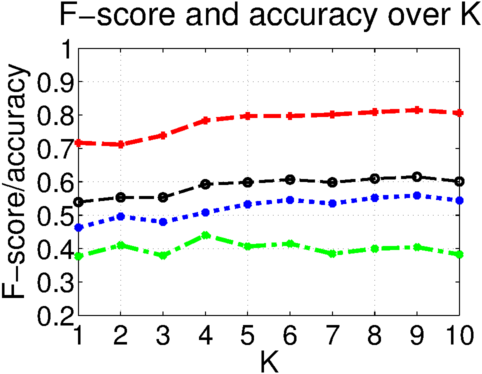
\includegraphics[width=0.3\textwidth]{tex/appendices/test/rms11FP.png}
	\centering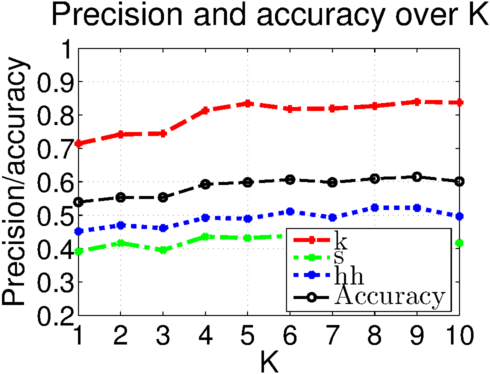
\includegraphics[width=0.3\textwidth]{tex/appendices/test/rms11_P.png}
	\centering\includegraphics[width=0.3\textwidth]{tex/appendices/test/rms11_R.png}
	
	\caption{Plots over K for Root Mean Square}
\end{figure}


\begin{table}
\begin{subtable}[tbp]{0.45\textwidth}
\centering
\begin{tabular}{|c|c|c|c"c|}
\cline{2-5}
 \multicolumn{1}{c|}{} & \textbf{k}  & \textbf{s}  & \textbf{hh}  & Prec.\\ \hline
 \textbf{k} & \textcolor{red}{0.719} & 0.212 & 0.161 & 0.714\\ \hline
 \textbf{s} & 0.094 & \textcolor{red}{0.364} & 0.364 & 0.391\\ \hline
 \textbf{hh} & 0.094 & 0.424 & \textcolor{red}{0.475} & 0.452\\ \Xhline{2\arrayrulewidth}
 F & 0.717 & 0.377 & 0.463 & \textcolor{blue}{0.539}\\ \hline
\end{tabular}
\label{app:RMS:1:worst}
\caption{$K=1$}
\end{subtable}
\hfill
\begin{subtable}[tbp]{0.45\textwidth}
\centering
\begin{tabular}{|c|c|c|c"c|}
\cline{2-5}
 \multicolumn{1}{c|}{} & \textbf{k}  & \textbf{s}  & \textbf{hh}  & Prec.\\ \hline
 \textbf{k} & \textcolor{red}{0.683} & 0.172 & 0.136 & 0.742\\ \hline
 \textbf{s} & 0.115 & \textcolor{red}{0.404} & 0.339 & 0.417\\ \hline
 \textbf{hh} & 0.115 & 0.424 & \textcolor{red}{0.525} & 0.470\\ \Xhline{2\arrayrulewidth}
 F & 0.712 & 0.410 & 0.496 & \textcolor{blue}{0.553}\\ \hline
\end{tabular}
\caption{$K=2$}
\end{subtable}
\hfill
\begin{subtable}[tbp]{0.45\textwidth}
\centering
\begin{tabular}{|c|c|c|c"c|}
\cline{2-5}
 \multicolumn{1}{c|}{} & \textbf{k}  & \textbf{s}  & \textbf{hh}  & Prec.\\ \hline
 \textbf{k} & \textcolor{red}{0.734} & 0.192 & 0.136 & 0.745\\ \hline
 \textbf{s} & 0.086 & \textcolor{red}{0.364} & 0.364 & 0.396\\ \hline
 \textbf{hh} & 0.086 & 0.444 & \textcolor{red}{0.500} & 0.461\\ \Xhline{2\arrayrulewidth}
 F & 0.739 & 0.379 & 0.480 & \textcolor{blue}{0.553}\\ \hline
\end{tabular}
\caption{$K=3$}
\end{subtable}
\hfill
\begin{subtable}[tbp]{0.45\textwidth}
\centering
\begin{tabular}{|c|c|c|c"c|}
\cline{2-5}
 \multicolumn{1}{c|}{} & \textbf{k}  & \textbf{s}  & \textbf{hh}  & Prec.\\ \hline
 \textbf{k} & \textcolor{red}{0.755} & 0.121 & 0.102 & 0.814\\ \hline
 \textbf{s} & 0.094 & \textcolor{red}{0.444} & 0.373 & 0.436\\ \hline
 \textbf{hh} & 0.094 & 0.434 & \textcolor{red}{0.525} & 0.492\\ \Xhline{2\arrayrulewidth}
 F & 0.784 & 0.440 & 0.508 & \textcolor{blue}{0.593}\\ \hline
\end{tabular}
\caption{$K=4$}
\end{subtable}
\hfill
\begin{subtable}[tbp]{0.45\textwidth}
\centering
\begin{tabular}{|c|c|c|c"c|}
\cline{2-5}
 \multicolumn{1}{c|}{} & \textbf{k}  & \textbf{s}  & \textbf{hh}  & Prec.\\ \hline
 \textbf{k} & \textcolor{red}{0.763} & 0.111 & 0.085 & 0.835\\ \hline
 \textbf{s} & 0.079 & \textcolor{red}{0.384} & 0.331 & 0.432\\ \hline
 \textbf{hh} & 0.079 & 0.505 & \textcolor{red}{0.585} & 0.489\\ \Xhline{2\arrayrulewidth}
 F & 0.797 & 0.406 & 0.533 & \textcolor{blue}{0.598}\\ \hline
\end{tabular}
\caption{$K=5$}
\end{subtable}
\hfill
\begin{subtable}[tbp]{0.45\textwidth}
\centering
\begin{tabular}{|c|c|c|c"c|}
\cline{2-5}
 \multicolumn{1}{c|}{} & \textbf{k}  & \textbf{s}  & \textbf{hh}  & Prec.\\ \hline
 \textbf{k} & \textcolor{red}{0.777} & 0.121 & 0.102 & 0.818\\ \hline
 \textbf{s} & 0.094 & \textcolor{red}{0.394} & 0.314 & 0.438\\ \hline
 \textbf{hh} & 0.094 & 0.485 & \textcolor{red}{0.585} & 0.511\\ \Xhline{2\arrayrulewidth}
 F & 0.797 & 0.415 & 0.545 & \textcolor{blue}{0.607}\\ \hline
\end{tabular}
\label{app:rms:k6}
\caption{$K=6$}
\end{subtable}
\hfill
\begin{subtable}[tbp]{0.45\textwidth}
\centering
\begin{tabular}{|c|c|c|c"c|}
\cline{2-5}
 \multicolumn{1}{c|}{} & \textbf{k}  & \textbf{s}  & \textbf{hh}  & Prec.\\ \hline
 \textbf{k} & \textcolor{red}{0.784} & 0.131 & 0.093 & 0.820\\ \hline
 \textbf{s} & 0.072 & \textcolor{red}{0.354} & 0.322 & 0.422\\ \hline
 \textbf{hh} & 0.072 & 0.515 & \textcolor{red}{0.585} & 0.493\\ \Xhline{2\arrayrulewidth}
 F & 0.801 & 0.385 & 0.535 & \textcolor{blue}{0.598}\\ \hline
\end{tabular}
\caption{$K=7$}
\end{subtable}
\hfill
\begin{subtable}[tbp]{0.45\textwidth}
\centering
\begin{tabular}{|c|c|c|c"c|}
\cline{2-5}
 \multicolumn{1}{c|}{} & \textbf{k}  & \textbf{s}  & \textbf{hh}  & Prec.\\ \hline
 \textbf{k} & \textcolor{red}{0.791} & 0.141 & 0.076 & 0.827\\ \hline
 \textbf{s} & 0.094 & \textcolor{red}{0.384} & 0.339 & 0.418\\ \hline
 \textbf{hh} & 0.094 & 0.475 & \textcolor{red}{0.585} & 0.523\\ \Xhline{2\arrayrulewidth}
 F & 0.809 & 0.400 & 0.552 & \textcolor{blue}{0.610}\\ \hline
\end{tabular}
\caption{$K=8$}
\label{app:rms:k8}
\end{subtable}
\hfill
\begin{subtable}[tbp]{0.45\textwidth}
\centering
\begin{tabular}{|c|c|c|c"c|}
\cline{2-5}
 \multicolumn{1}{c|}{} & \textbf{k}  & \textbf{s}  & \textbf{hh}  & Prec.\\ \hline
 \textbf{k} & \textcolor{red}{0.791} & 0.141 & 0.059 & 0.840\\ \hline
 \textbf{s} & 0.079 & \textcolor{red}{0.384} & 0.339 & 0.427\\ \hline
 \textbf{hh} & 0.079 & 0.475 & \textcolor{red}{0.602} & 0.522\\ \Xhline{2\arrayrulewidth}
 F & 0.815 & 0.404 & 0.559 & \textcolor{blue}{0.615}\\ \hline
\end{tabular}
\label{app:RMS:9:best}
\caption{$K=9$}
\end{subtable}
\hfill
\begin{subtable}[tbp]{0.45\textwidth}
\centering
\begin{tabular}{|c|c|c|c"c|}
\cline{2-5}
 \multicolumn{1}{c|}{} & \textbf{k}  & \textbf{s}  & \textbf{hh}  & Prec.\\ \hline
 \textbf{k} & \textcolor{red}{0.777} & 0.121 & 0.076 & 0.837\\ \hline
 \textbf{s} & 0.079 & \textcolor{red}{0.354} & 0.322 & 0.417\\ \hline
 \textbf{hh} & 0.079 & 0.525 & \textcolor{red}{0.602} & 0.497\\ \Xhline{2\arrayrulewidth}
 F & 0.806 & 0.383 & 0.544 & \textcolor{blue}{0.601}\\ \hline
\end{tabular}
\caption{$K=10$}
\end{subtable}
\hfill

\label{tlrms11}

\caption{tcrms11}

\end{table}\clearpage


\begin{table}

\begin{subtable}[h]{0.45\textwidth}
\centering
 \scalebox{0.8}{
\begin{tabular}{|c|c|c|c|}\hline
 $K_1$ & $K_2$ & $X^2$ & p\\ \hline
 1 & 2 & 54.000 & 0.25605\\ \hline 
 1 & 3 & 72.000 & 0.23040\\ \hline 
 1 & 4 & 54.000 & 0.25605\\ \hline 
 1 & 5 & 63.000 & 0.24255\\ \hline 
 1 & 6 & 63.000 & 0.24255\\ \hline 
 1 & 7 & 72.000 & 0.23040\\ \hline 
 1 & 8 & 72.000 & 0.23040\\ \hline 
 1 & 9 & 72.000 & 0.23040\\ \hline 
 1 & 10 & 72.000 & 0.23040\\ \hline 
 2 & 3 & 54.000 & 0.25605\\ \hline 
 2 & 4 & 47.250 & 0.09945\\ \hline 
 2 & 5 & 47.250 & 0.26685\\ \hline 
 2 & 6 & 47.250 & 0.26685\\ \hline 
 2 & 7 & 54.000 & 0.25605\\ \hline 
 2 & 8 & 54.000 & 0.25605\\ \hline 
 2 & 9 & 54.000 & 0.25605\\ \hline 
 2 & 10 & 54.000 & 0.25605\\ \hline 
 3 & 4 & 54.000 & 0.25605\\ \hline 
 3 & 5 & 63.000 & 0.24255\\ \hline 
 3 & 6 & 63.000 & 0.24255\\ \hline 
 3 & 7 & 72.000 & 0.23040\\ \hline 
 3 & 8 & 72.000 & 0.23040\\ \hline 
 3 & 9 & 72.000 & 0.23040\\ \hline 
 3 & 10 & 72.000 & 0.23040\\ \hline 
 4 & 5 & 47.250 & 0.26685\\ \hline 
 4 & 6 & 54.000 & 0.00225\\ \hline 
 4 & 7 & 54.000 & 0.25605\\ \hline 
 4 & 8 & 54.000 & 0.25605\\ \hline 
 4 & 9 & 54.000 & 0.25605\\ \hline 
 4 & 10 & 54.000 & 0.25605\\ \hline 
 5 & 6 & 56.250 & 0.022185\\ \hline 
 5 & 7 & 63.000 & 0.24255\\ \hline 
 5 & 8 & 63.000 & 0.24255\\ \hline 
 5 & 9 & 63.000 & 0.24255\\ \hline 
 5 & 10 & 63.000 & 0.24255\\ \hline 
 6 & 7 & 63.000 & 0.24255\\ \hline 
 6 & 8 & 63.000 & 0.24255\\ \hline 
 6 & 9 & 63.000 & 0.24255\\ \hline 
 6 & 10 & 63.000 & 0.24255\\ \hline 
 7 & 8 & 72.000 & 0.23040\\ \hline 
 7 & 9 & 72.000 & 0.23040\\ \hline 
 7 & 10 & 72.000 & 0.23040\\ \hline 
 8 & 9 & 72.000 & 0.23040\\ \hline 
 8 & 10 & 72.000 & 0.23040\\ \hline 
 9 & 10 & 72.000 & 0.23040\\ \hline 

\end{tabular}
} \label{xlrms11}
\caption{xcrms11}
\end{subtable}

\begin{subtable}[h]{0.45\textwidth}
\centering
\begin{tabular}{|c|c|c|}
\hline
Class & Amount & Percent\\ \hline
k & 326 & 39.14\\ \hline
s & 231 & 27.73\\ \hline
hh & 276 & 33.13\\ \hline
\end{tabular}
\caption{Training dataset}
\end{subtable}
\hfill
\begin{subtable}[h]{0.45\textwidth}
\centering
\begin{tabular}{|c|c|c|}
\hline
Class & Amount & Percent\\ \hline
k & 139 & 39.04\\ \hline
s & 99 & 27.81\\ \hline
hh & 118 & 33.15\\ \hline
\end{tabular}
\caption{Testing dataset}
\end{subtable}
\hfill

\label{dlrms11}

\caption{dcrms11}

\end{table}

\subsection{ZCR}
	\label{app:res:zrc}
	\begin{figure}
	\centering\includegraphics[width=0.3\textwidth]{tex/appendices/test/zcr11FP.png}
	\centering\includegraphics[width=0.3\textwidth]{tex/appendices/test/zcr11_P.png}
	\centering\includegraphics[width=0.3\textwidth]{tex/appendices/test/zcr11_R.png}
	\caption{Plots over K for Zero Crossing Rate}
\end{figure}


\begin{table}
\begin{subtable}[tbp]{0.45\textwidth}
\centering
\begin{tabular}{|c|c|c|c"c|}
\cline{2-5}
 \multicolumn{1}{c|}{} & \textbf{k}  & \textbf{s}  & \textbf{hh}  & Prec.\\ \hline
 \textbf{k} & \textcolor{red}{0.899} & 0.172 & 0.051 & 0.845\\ \hline
 \textbf{s} & 0.101 & \textcolor{red}{0.525} & 0.288 & 0.520\\ \hline
 \textbf{hh} & 0.101 & 0.303 & \textcolor{red}{0.661} & 0.722\\ \Xhline{2\arrayrulewidth}
 F & 0.871 & 0.523 & 0.690 & \textcolor{blue}{0.716}\\ \hline
\end{tabular}
\caption{$K=1$}
\end{subtable}
\hfill
\begin{subtable}[tbp]{0.45\textwidth}
\centering
\begin{tabular}{|c|c|c|c"c|}
\cline{2-5}
 \multicolumn{1}{c|}{} & \textbf{k}  & \textbf{s}  & \textbf{hh}  & Prec.\\ \hline
 \textbf{k} & \textcolor{red}{0.885} & 0.162 & 0.042 & 0.854\\ \hline
 \textbf{s} & 0.108 & \textcolor{red}{0.475} & 0.305 & 0.480\\ \hline
 \textbf{hh} & 0.108 & 0.364 & \textcolor{red}{0.653} & 0.675\\ \Xhline{2\arrayrulewidth}
 F & 0.869 & 0.477 & 0.664 & \textcolor{blue}{0.694}\\ \hline
\end{tabular}
\caption{$K=2$}
\label{app-ZCR-Worst}
\end{subtable}
\hfill
\begin{subtable}[tbp]{0.45\textwidth}
\centering
\begin{tabular}{|c|c|c|c"c|}
\cline{2-5}
 \multicolumn{1}{c|}{} & \textbf{k}  & \textbf{s}  & \textbf{hh}  & Prec.\\ \hline
 \textbf{k} & \textcolor{red}{0.914} & 0.141 & 0.042 & 0.870\\ \hline
 \textbf{s} & 0.086 & \textcolor{red}{0.576} & 0.220 & 0.600\\ \hline
 \textbf{hh} & 0.086 & 0.283 & \textcolor{red}{0.737} & 0.757\\ \Xhline{2\arrayrulewidth}
 F & 0.891 & 0.588 & 0.747 & \textcolor{blue}{0.761}\\ \hline
\end{tabular}
\caption{$K=3$}
\end{subtable}
\hfill
\begin{subtable}[tbp]{0.45\textwidth}
\centering
\begin{tabular}{|c|c|c|c"c|}
\cline{2-5}
 \multicolumn{1}{c|}{} & \textbf{k}  & \textbf{s}  & \textbf{hh}  & Prec.\\ \hline
 \textbf{k} & \textcolor{red}{0.899} & 0.131 & 0.025 & 0.887\\ \hline
 \textbf{s} & 0.101 & \textcolor{red}{0.525} & 0.229 & 0.559\\ \hline
 \textbf{hh} & 0.101 & 0.343 & \textcolor{red}{0.746} & 0.721\\ \Xhline{2\arrayrulewidth}
 F & 0.893 & 0.542 & 0.733 & \textcolor{blue}{0.744}\\ \hline
\end{tabular}
\caption{$K=4$}
\end{subtable}
\hfill
\begin{subtable}[tbp]{0.45\textwidth}
\centering
\begin{tabular}{|c|c|c|c"c|}
\cline{2-5}
 \multicolumn{1}{c|}{} & \textbf{k}  & \textbf{s}  & \textbf{hh}  & Prec.\\ \hline
 \textbf{k} & \textcolor{red}{0.892} & 0.101 & 0.017 & 0.912\\ \hline
 \textbf{s} & 0.108 & \textcolor{red}{0.545} & 0.212 & 0.574\\ \hline
 \textbf{hh} & 0.108 & 0.354 & \textcolor{red}{0.771} & 0.722\\ \Xhline{2\arrayrulewidth}
 F & 0.902 & 0.560 & 0.746 & \textcolor{blue}{0.756}\\ \hline
\end{tabular}
\caption{$K=5$}
\end{subtable}
\hfill
\begin{subtable}[tbp]{0.45\textwidth}
\centering
\begin{tabular}{|c|c|c|c"c|}
\cline{2-5}
 \multicolumn{1}{c|}{} & \textbf{k}  & \textbf{s}  & \textbf{hh}  & Prec.\\ \hline
 \textbf{k} & \textcolor{red}{0.906} & 0.091 & 0.017 & 0.920\\ \hline
 \textbf{s} & 0.094 & \textcolor{red}{0.566} & 0.186 & 0.615\\ \hline
 \textbf{hh} & 0.094 & 0.343 & \textcolor{red}{0.797} & 0.734\\ \Xhline{2\arrayrulewidth}
 F & 0.913 & 0.589 & 0.764 & \textcolor{blue}{0.775}\\ \hline
\end{tabular}
\caption{$K=6$}
\end{subtable}
\hfill
\begin{subtable}[tbp]{0.45\textwidth}
\centering
\begin{tabular}{|c|c|c|c"c|}
\cline{2-5}
 \multicolumn{1}{c|}{} & \textbf{k}  & \textbf{s}  & \textbf{hh}  & Prec.\\ \hline
 \textbf{k} & \textcolor{red}{0.892} & 0.071 & 0.017 & 0.932\\ \hline
 \textbf{s} & 0.108 & \textcolor{red}{0.576} & 0.178 & 0.613\\ \hline
 \textbf{hh} & 0.108 & 0.354 & \textcolor{red}{0.805} & 0.731\\ \Xhline{2\arrayrulewidth}
 F & 0.912 & 0.594 & 0.766 & \textcolor{blue}{0.775}\\ \hline
\end{tabular}
\caption{$K=7$}
\end{subtable}
\hfill
\begin{subtable}[tbp]{0.45\textwidth}
\centering
\begin{tabular}{|c|c|c|c"c|}
\cline{2-5}
 \multicolumn{1}{c|}{} & \textbf{k}  & \textbf{s}  & \textbf{hh}  & Prec.\\ \hline
 \textbf{k} & \textcolor{red}{0.892} & 0.091 & 0.017 & 0.919\\ \hline
 \textbf{s} & 0.101 & \textcolor{red}{0.596} & 0.178 & 0.628\\ \hline
 \textbf{hh} & 0.101 & 0.313 & \textcolor{red}{0.805} & 0.748\\ \Xhline{2\arrayrulewidth}
 F & 0.905 & 0.611 & 0.776 & \textcolor{blue}{0.781}\\ \hline
\end{tabular}
\caption{$K=8$}
\end{subtable}
\hfill
\begin{subtable}[tbp]{0.45\textwidth}
\centering
\begin{tabular}{|c|c|c|c"c|}
\cline{2-5}
 \multicolumn{1}{c|}{} & \textbf{k}  & \textbf{s}  & \textbf{hh}  & Prec.\\ \hline
 \textbf{k} & \textcolor{red}{0.871} & 0.081 & 0.017 & 0.924\\ \hline
 \textbf{s} & 0.122 & \textcolor{red}{0.636} & 0.169 & 0.630\\ \hline
 \textbf{hh} & 0.122 & 0.283 & \textcolor{red}{0.814} & 0.768\\ \Xhline{2\arrayrulewidth}
 F & 0.896 & 0.633 & 0.790 & \textcolor{blue}{0.787}\\ \hline
\end{tabular}
\caption{$K=9$}
\label{app:zcr:best}
\end{subtable}
\hfill
\begin{subtable}[tbp]{0.45\textwidth}
\centering
\begin{tabular}{|c|c|c|c"c|}
\cline{2-5}
 \multicolumn{1}{c|}{} & \textbf{k}  & \textbf{s}  & \textbf{hh}  & Prec.\\ \hline
 \textbf{k} & \textcolor{red}{0.871} & 0.051 & 0.017 & 0.945\\ \hline
 \textbf{s} & 0.122 & \textcolor{red}{0.636} & 0.169 & 0.630\\ \hline
 \textbf{hh} & 0.122 & 0.313 & \textcolor{red}{0.814} & 0.750\\ \Xhline{2\arrayrulewidth}
 F & 0.906 & 0.633 & 0.780 & \textcolor{blue}{0.787}\\ \hline
\end{tabular}
\caption{$K=10$}
\label{app:zcr:best2}
\end{subtable}
\hfill

\caption{tczcr11}

\label{tlzcr11}

\end{table}\clearpage


\begin{table}

\begin{subtable}[tbp]{0.4\textwidth}
\centering
 
\begin{tabular}{|c|c|c|c|}\hline
 $K_1$ & $K_2$ & $X^2$ & p\\ \hline
 1 & 2 & 63.000 & 0.24255\\ \hline 
 1 & 3 & 72.000 & 0.2304\\ \hline 
 1 & 4 & 72.000 & 0.2304\\ \hline 
 1 & 5 & 72.000 & 0.2304\\ \hline 
 1 & 6 & 72.000 & 0.2304\\ \hline 
 1 & 7 & 72.000 & 0.2304\\ \hline 
 1 & 8 & 72.000 & 0.2304\\ \hline 
 1 & 9 & 72.000 & 0.2304\\ \hline 
 1 & 10 & 72.000 & 0.2304\\ \hline 
 2 & 3 & 63.000 & 0.24255\\ \hline 
 2 & 4 & 63.000 & 0.24255\\ \hline 
 2 & 5 & 63.000 & 0.24255\\ \hline 
 2 & 6 & 63.000 & 0.24255\\ \hline 
 2 & 7 & 63.000 & 0.24255\\ \hline 
 2 & 8 & 63.000 & 0.24255\\ \hline 
 2 & 9 & 63.000 & 0.24255\\ \hline 
 2 & 10 & 63.000 & 0.24255\\ \hline 
 3 & 4 & 72.000 & 0.2304\\ \hline 
 3 & 5 & 72.000 & 0.2304\\ \hline 
 3 & 6 & 72.000 & 0.2304\\ \hline 
 3 & 7 & 72.000 & 0.2304\\ \hline 
 3 & 8 & 72.000 & 0.2304\\ \hline 
 3 & 9 & 72.000 & 0.2304\\ \hline 
 3 & 10 & 72.000 & 0.2304\\ \hline 
 4 & 5 & 72.000 & 0.2304\\ \hline 
 4 & 6 & 72.000 & 0.2304\\ \hline 
 4 & 7 & 72.000 & 0.2304\\ \hline 
 4 & 8 & 72.000 & 0.2304\\ \hline 
 4 & 9 & 72.000 & 0.2304\\ \hline 
 4 & 10 & 72.000 & 0.2304\\ \hline 
 5 & 6 & 72.000 & 0.2304\\ \hline 
 5 & 7 & 72.000 & 0.2304\\ \hline 
 5 & 8 & 72.000 & 0.2304\\ \hline 
 5 & 9 & 72.000 & 0.2304\\ \hline 
 5 & 10 & 72.000 & 0.2304\\ \hline 
 6 & 7 & 72.000 & 0.2304\\ \hline 
 6 & 8 & 72.000 & 0.2304\\ \hline 
 6 & 9 & 72.000 & 0.2304\\ \hline 
 6 & 10 & 72.000 & 0.2304\\ \hline 
 7 & 8 & 72.000 & 0.2304\\ \hline 
 7 & 9 & 72.000 & 0.2304\\ \hline 
 7 & 10 & 72.000 & 0.2304\\ \hline 
 8 & 9 & 72.000 & 0.2304\\ \hline 
 8 & 10 & 72.000 & 0.2304\\ \hline 
 9 & 10 & 72.000 & 0.2304\\ \hline 

\end{tabular}
\caption{xczcr11}
 \label{xlzcr11}
\end{subtable}


\begin{subtable}[h]{0.45\textwidth}
\centering
\begin{tabular}{|c|c|c|}
\hline
Class & Amount & Percent\\ \hline
k & 326 & 39.14\\ \hline
s & 231 & 27.73\\ \hline
hh & 276 & 33.13\\ \hline
\end{tabular}
\caption{Training dataset}
\end{subtable}
\hfill
\begin{subtable}[h]{0.45\textwidth}
\centering
\begin{tabular}{|c|c|c|}
\hline
Class & Amount & Percent\\ \hline
k & 139 & 39.04\\ \hline
s & 99 & 27.81\\ \hline
hh & 118 & 33.15\\ \hline
\end{tabular}
\caption{Testing dataset}
\end{subtable}
\hfill


\caption{dczcr11}
\label{dlzcr11}

\end{table}\clearpage
	
\subsection{MFCC}
	\label{app:res:mfcc}
	\begin{figure}


	\centering\includegraphics[width=0.3\textwidth]{tex/appendices/test/mfcc2010FP.png}
	\centering\includegraphics[width=0.3\textwidth]{tex/appendices/test/mfcc2010_P.png}
	\centering\includegraphics[width=0.3\textwidth]{tex/appendices/test/mfcc2010_R.png}
	
	\caption{Plots over K for MFCC with 20ms windows and 10ms window skips}
\end{figure}
\begin{figure}


	\centering\includegraphics[width=0.3\textwidth]{tex/appendices/test/mfcc105FP.png}
	\centering\includegraphics[width=0.3\textwidth]{tex/appendices/test/mfcc105_P.png}
	\centering\includegraphics[width=0.3\textwidth]{tex/appendices/test/mfcc105_R.png}
	
	\caption{Plots over K for MFCC with 10ms windows and 5ms window skips}
\end{figure}
\begin{figure}


	\centering\includegraphics[width=0.3\textwidth]{tex/appendices/test/mfcc52FP.png}
	\centering\includegraphics[width=0.3\textwidth]{tex/appendices/test/mfcc52_P.png}
	\centering\includegraphics[width=0.3\textwidth]{tex/appendices/test/mfcc52_R.png}
	
	\caption{Plots over K for MFCC with 5ms windows and 2ms window skips}
\end{figure}\clearpage


\begin{table}
\begin{subtable}[tbp]{0.45\textwidth}
\centering
\begin{tabular}{|c|c|c|c"c|}
\cline{2-5}
 \multicolumn{1}{c|}{} & \textbf{k}  & \textbf{s}  & \textbf{hh}  & Prec.\\ \hline
 \textbf{k} & \textcolor{red}{0.986} & 0.054 & 0.000 & 0.965\\ \hline
 \textbf{s} & 0.007 & \textcolor{red}{0.891} & 0.026 & 0.953\\ \hline
 \textbf{hh} & 0.007 & 0.054 & \textcolor{red}{0.974} & 0.950\\ \Xhline{2\arrayrulewidth}
 F & 0.975 & 0.921 & 0.962 & \textcolor{blue}{0.957}\\ \hline
\end{tabular}
\caption{$K=1$}
\end{subtable}
\hfill
\begin{subtable}[tbp]{0.45\textwidth}
\centering
\begin{tabular}{|c|c|c|c"c|}
\cline{2-5}
 \multicolumn{1}{c|}{} & \textbf{k}  & \textbf{s}  & \textbf{hh}  & Prec.\\ \hline
 \textbf{k} & \textcolor{red}{0.986} & 0.043 & 0.000 & 0.971\\ \hline
 \textbf{s} & 0.007 & \textcolor{red}{0.913} & 0.060 & 0.913\\ \hline
 \textbf{hh} & 0.007 & 0.043 & \textcolor{red}{0.940} & 0.957\\ \Xhline{2\arrayrulewidth}
 F & 0.978 & 0.913 & 0.948 & \textcolor{blue}{0.951}\\ \hline
\end{tabular}
\caption{$K=2$}
\end{subtable}
\hfill
\begin{subtable}[tbp]{0.45\textwidth}
\centering
\begin{tabular}{|c|c|c|c"c|}
\cline{2-5}
 \multicolumn{1}{c|}{} & \textbf{k}  & \textbf{s}  & \textbf{hh}  & Prec.\\ \hline
 \textbf{k} & \textcolor{red}{1.000} & 0.043 & 0.000 & 0.972\\ \hline
 \textbf{s} & 0.000 & \textcolor{red}{0.924} & 0.026 & 0.966\\ \hline
 \textbf{hh} & 0.000 & 0.033 & \textcolor{red}{0.974} & 0.974\\ \Xhline{2\arrayrulewidth}
 F & 0.986 & 0.944 & 0.974 & \textcolor{blue}{0.971}\\ \hline
\end{tabular}
\caption{$K=3$}
\end{subtable}
\hfill
\begin{subtable}[tbp]{0.45\textwidth}
\centering
\begin{tabular}{|c|c|c|c"c|}
\cline{2-5}
 \multicolumn{1}{c|}{} & \textbf{k}  & \textbf{s}  & \textbf{hh}  & Prec.\\ \hline
 \textbf{k} & \textcolor{red}{1.000} & 0.054 & 0.000 & 0.965\\ \hline
 \textbf{s} & 0.000 & \textcolor{red}{0.902} & 0.034 & 0.954\\ \hline
 \textbf{hh} & 0.000 & 0.043 & \textcolor{red}{0.966} & 0.966\\ \Xhline{2\arrayrulewidth}
 F & 0.982 & 0.927 & 0.966 & \textcolor{blue}{0.963}\\ \hline
\end{tabular}
\caption{$K=4$}
\end{subtable}
\hfill
\begin{subtable}[tbp]{0.45\textwidth}
\centering
\begin{tabular}{|c|c|c|c"c|}
\cline{2-5}
 \multicolumn{1}{c|}{} & \textbf{k}  & \textbf{s}  & \textbf{hh}  & Prec.\\ \hline
 \textbf{k} & \textcolor{red}{1.000} & 0.043 & 0.000 & 0.972\\ \hline
 \textbf{s} & 0.000 & \textcolor{red}{0.913} & 0.034 & 0.955\\ \hline
 \textbf{hh} & 0.000 & 0.043 & \textcolor{red}{0.966} & 0.966\\ \Xhline{2\arrayrulewidth}
 F & 0.986 & 0.933 & 0.966 & \textcolor{blue}{0.965}\\ \hline
\end{tabular}
\caption{$K=5$}
\end{subtable}
\hfill
\begin{subtable}[tbp]{0.45\textwidth}
\centering
\begin{tabular}{|c|c|c|c"c|}
\cline{2-5}
 \multicolumn{1}{c|}{} & \textbf{k}  & \textbf{s}  & \textbf{hh}  & Prec.\\ \hline
 \textbf{k} & \textcolor{red}{0.993} & 0.043 & 0.009 & 0.965\\ \hline
 \textbf{s} & 0.000 & \textcolor{red}{0.913} & 0.034 & 0.955\\ \hline
 \textbf{hh} & 0.000 & 0.043 & \textcolor{red}{0.957} & 0.957\\ \Xhline{2\arrayrulewidth}
 F & 0.979 & 0.933 & 0.957 & \textcolor{blue}{0.960}\\ \hline
\end{tabular}
\caption{$K=6$}
\end{subtable}
\hfill
\begin{subtable}[tbp]{0.45\textwidth}
\centering
\begin{tabular}{|c|c|c|c"c|}
\cline{2-5}
 \multicolumn{1}{c|}{} & \textbf{k}  & \textbf{s}  & \textbf{hh}  & Prec.\\ \hline
 \textbf{k} & \textcolor{red}{0.993} & 0.054 & 0.009 & 0.958\\ \hline
 \textbf{s} & 0.007 & \textcolor{red}{0.902} & 0.034 & 0.943\\ \hline
 \textbf{hh} & 0.007 & 0.043 & \textcolor{red}{0.957} & 0.966\\ \Xhline{2\arrayrulewidth}
 F & 0.975 & 0.922 & 0.961 & \textcolor{blue}{0.957}\\ \hline
\end{tabular}
\caption{$K=7$}
\end{subtable}
\hfill
\begin{subtable}[tbp]{0.45\textwidth}
\centering
\begin{tabular}{|c|c|c|c"c|}
\cline{2-5}
 \multicolumn{1}{c|}{} & \textbf{k}  & \textbf{s}  & \textbf{hh}  & Prec.\\ \hline
 \textbf{k} & \textcolor{red}{1.000} & 0.054 & 0.009 & 0.958\\ \hline
 \textbf{s} & 0.000 & \textcolor{red}{0.902} & 0.034 & 0.954\\ \hline
 \textbf{hh} & 0.000 & 0.043 & \textcolor{red}{0.957} & 0.966\\ \Xhline{2\arrayrulewidth}
 F & 0.979 & 0.927 & 0.961 & \textcolor{blue}{0.960}\\ \hline
\end{tabular}
\caption{$K=8$}
\end{subtable}
\hfill
\begin{subtable}[tbp]{0.45\textwidth}
\centering
\begin{tabular}{|c|c|c|c"c|}
\cline{2-5}
 \multicolumn{1}{c|}{} & \textbf{k}  & \textbf{s}  & \textbf{hh}  & Prec.\\ \hline
 \textbf{k} & \textcolor{red}{1.000} & 0.054 & 0.009 & 0.958\\ \hline
 \textbf{s} & 0.000 & \textcolor{red}{0.913} & 0.026 & 0.966\\ \hline
 \textbf{hh} & 0.000 & 0.033 & \textcolor{red}{0.966} & 0.974\\ \Xhline{2\arrayrulewidth}
 F & 0.979 & 0.939 & 0.970 & \textcolor{blue}{0.965}\\ \hline
\end{tabular}
\caption{$K=9$}
\end{subtable}
\hfill
\begin{subtable}[tbp]{0.45\textwidth}
\centering
\begin{tabular}{|c|c|c|c"c|}
\cline{2-5}
 \multicolumn{1}{c|}{} & \textbf{k}  & \textbf{s}  & \textbf{hh}  & Prec.\\ \hline
 \textbf{k} & \textcolor{red}{1.000} & 0.054 & 0.009 & 0.958\\ \hline
 \textbf{s} & 0.000 & \textcolor{red}{0.913} & 0.026 & 0.966\\ \hline
 \textbf{hh} & 0.000 & 0.033 & \textcolor{red}{0.966} & 0.974\\ \Xhline{2\arrayrulewidth}
 F & 0.979 & 0.939 & 0.970 & \textcolor{blue}{0.965}\\ \hline
\end{tabular}
\caption{$K=10$}
\end{subtable}
\hfill

\label{tlmfcc2010}

\caption{tcmfcc2010}

\end{table}\clearpage


\begin{table}

\begin{subtable}[tbp]{0.45\textwidth}
\centering
 
\scalebox{0.8}{\begin{tabular}{|c|c|c|c|}\hline
 $K_1$ & $K_2$ & $X^2$ & p\\ \hline
 1 & 2 & 54.000 & 0.00061\\ \hline 
 1 & 3 & 38.250 & 0.00319\\ \hline 
 1 & 4 & 38.250 & 0.00319\\ \hline 
 1 & 5 & 36.000 & 0.00122\\ \hline 
 1 & 6 & 38.250 & 0.00319\\ \hline 
 1 & 7 & 40.500 & 0.00619\\ \hline 
 1 & 8 & 47.250 & 0.00221\\ \hline 
 1 & 9 & 47.250 & 0.00221\\ \hline 
 1 & 10 & 47.250 & 0.00221\\ \hline 
 2 & 3 & 38.250 & 0.00319\\ \hline 
 2 & 4 & 38.250 & 0.00319\\ \hline 
 2 & 5 & 36.000 & 0.00122\\ \hline 
 2 & 6 & 38.250 & 0.00319\\ \hline 
 2 & 7 & 40.500 & 0.00619\\ \hline 
 2 & 8 & 47.250 & 0.00221\\ \hline 
 2 & 9 & 47.250 & 0.00221\\ \hline 
 2 & 10 & 47.250 & 0.00221\\ \hline 
 3 & 4 & 45.000 & 0.00019\\ \hline 
 3 & 5 & 36.000 & 0.00034\\ \hline 
 3 & 6 & 36.000 & 0.00159\\ \hline 
 3 & 7 & 45.000 & 0.00086\\ \hline 
 3 & 8 & 45.000 & 0.00086\\ \hline 
 3 & 9 & 45.000 & 0.00086\\ \hline 
 3 & 10 & 45.000 & 0.00086\\ \hline 
 4 & 5 & 36.000 & 0.00034\\ \hline 
 4 & 6 & 36.000 & 0.00159\\ \hline 
 4 & 7 & 45.000 & 0.00086\\ \hline 
 4 & 8 & 45.000 & 0.00086\\ \hline 
 4 & 9 & 45.000 & 0.00086\\ \hline 
 4 & 10 & 45.000 & 0.00086\\ \hline 
 5 & 6 & 36.000 & 0.00034\\ \hline 
 5 & 7 & 36.000 & 0.00122\\ \hline 
 5 & 8 & 36.000 & 0.00122\\ \hline 
 5 & 9 & 36.000 & 0.00122\\ \hline 
 5 & 10 & 36.000 & 0.00122\\ \hline 
 6 & 7 & 38.250 & 0.00319\\ \hline 
 6 & 8 & 38.250 & 0.00319\\ \hline 
 6 & 9 & 38.250 & 0.00319\\ \hline 
 6 & 10 & 38.250 & 0.00319\\ \hline 
 7 & 8 & 47.250 & 0.00221\\ \hline 
 7 & 9 & 47.250 & 0.00221\\ \hline 
 7 & 10 & 47.250 & 0.00221\\ \hline 
 8 & 9 & 54.000 & 0.00061\\ \hline 
 8 & 10 & 54.000 & 0.00061\\ \hline 
 9 & 10 & 54.000 & 0.00061\\ \hline 

\end{tabular}
} \label{xlmfcc2010}
\caption{xcmfcc2010}
\end{subtable}

\begin{subtable}[tbp]{0.45\textwidth}
\centering
\begin{tabular}{|c|c|c|}
\hline
Class & Amount & Percent\\ \hline
k & 322 & 39.80\\ \hline
s & 214 & 26.45\\ \hline
hh & 273 & 33.75\\ \hline
\end{tabular}
\caption{Training dataset}
\end{subtable}
\hfill
\begin{subtable}[tbp]{0.45\textwidth}
\centering
\begin{tabular}{|c|c|c|}
\hline
Class & Amount & Percent\\ \hline
k & 138 & 39.77\\ \hline
s & 92 & 26.51\\ \hline
hh & 117 & 33.72\\ \hline
\end{tabular}
\caption{Testing dataset}
\end{subtable}
\hfill

\label{dlmfcc2010}

\caption{dcmfcc2010}

\end{table}\clearpage


\begin{table}
\begin{subtable}[tbp]{0.45\textwidth}
\centering
\begin{tabular}{|c|c|c|c"c|}
\cline{2-5}
 \multicolumn{1}{c|}{} & \textbf{k}  & \textbf{s}  & \textbf{hh}  & Prec.\\ \hline
 \textbf{k} & \textcolor{red}{0.978} & 0.031 & 0.017 & 0.965\\ \hline
 \textbf{s} & 0.022 & \textcolor{red}{0.929} & 0.034 & 0.929\\ \hline
 \textbf{hh} & 0.022 & 0.041 & \textcolor{red}{0.949} & 0.966\\ \Xhline{2\arrayrulewidth}
 F & 0.971 & 0.929 & 0.957 & \textcolor{blue}{0.955}\\ \hline
\end{tabular}
\caption{$K=1$}
\end{subtable}
\hfill
\begin{subtable}[tbp]{0.45\textwidth}
\centering
\begin{tabular}{|c|c|c|c"c|}
\cline{2-5}
 \multicolumn{1}{c|}{} & \textbf{k}  & \textbf{s}  & \textbf{hh}  & Prec.\\ \hline
 \textbf{k} & \textcolor{red}{0.978} & 0.010 & 0.017 & 0.978\\ \hline
 \textbf{s} & 0.022 & \textcolor{red}{0.959} & 0.025 & 0.940\\ \hline
 \textbf{hh} & 0.022 & 0.031 & \textcolor{red}{0.958} & 0.974\\ \Xhline{2\arrayrulewidth}
 F & 0.978 & 0.949 & 0.966 & \textcolor{blue}{0.966}\\ \hline
\end{tabular}
\caption{$K=2$}
\end{subtable}
\hfill
\begin{subtable}[tbp]{0.45\textwidth}
\centering
\begin{tabular}{|c|c|c|c"c|}
\cline{2-5}
 \multicolumn{1}{c|}{} & \textbf{k}  & \textbf{s}  & \textbf{hh}  & Prec.\\ \hline
 \textbf{k} & \textcolor{red}{0.993} & 0.020 & 0.017 & 0.972\\ \hline
 \textbf{s} & 0.007 & \textcolor{red}{0.939} & 0.025 & 0.958\\ \hline
 \textbf{hh} & 0.007 & 0.041 & \textcolor{red}{0.958} & 0.966\\ \Xhline{2\arrayrulewidth}
 F & 0.982 & 0.948 & 0.962 & \textcolor{blue}{0.966}\\ \hline
\end{tabular}
\caption{$K=3$}
\end{subtable}
\hfill
\begin{subtable}[tbp]{0.45\textwidth}
\centering
\begin{tabular}{|c|c|c|c"c|}
\cline{2-5}
 \multicolumn{1}{c|}{} & \textbf{k}  & \textbf{s}  & \textbf{hh}  & Prec.\\ \hline
 \textbf{k} & \textcolor{red}{0.986} & 0.010 & 0.017 & 0.979\\ \hline
 \textbf{s} & 0.014 & \textcolor{red}{0.959} & 0.025 & 0.949\\ \hline
 \textbf{hh} & 0.014 & 0.031 & \textcolor{red}{0.958} & 0.974\\ \Xhline{2\arrayrulewidth}
 F & 0.982 & 0.954 & 0.966 & \textcolor{blue}{0.969}\\ \hline
\end{tabular}
\caption{$K=4$}
\end{subtable}
\hfill
\begin{subtable}[tbp]{0.45\textwidth}
\centering
\begin{tabular}{|c|c|c|c"c|}
\cline{2-5}
 \multicolumn{1}{c|}{} & \textbf{k}  & \textbf{s}  & \textbf{hh}  & Prec.\\ \hline
 \textbf{k} & \textcolor{red}{0.993} & 0.010 & 0.017 & 0.979\\ \hline
 \textbf{s} & 0.007 & \textcolor{red}{0.949} & 0.025 & 0.959\\ \hline
 \textbf{hh} & 0.007 & 0.041 & \textcolor{red}{0.958} & 0.966\\ \Xhline{2\arrayrulewidth}
 F & 0.986 & 0.954 & 0.962 & \textcolor{blue}{0.969}\\ \hline
\end{tabular}
\caption{$K=5$}
\end{subtable}
\hfill
\begin{subtable}[tbp]{0.45\textwidth}
\centering
\begin{tabular}{|c|c|c|c"c|}
\cline{2-5}
 \multicolumn{1}{c|}{} & \textbf{k}  & \textbf{s}  & \textbf{hh}  & Prec.\\ \hline
 \textbf{k} & \textcolor{red}{0.993} & 0.010 & 0.017 & 0.979\\ \hline
 \textbf{s} & 0.007 & \textcolor{red}{0.949} & 0.025 & 0.959\\ \hline
 \textbf{hh} & 0.007 & 0.041 & \textcolor{red}{0.958} & 0.966\\ \Xhline{2\arrayrulewidth}
 F & 0.986 & 0.954 & 0.962 & \textcolor{blue}{0.969}\\ \hline
\end{tabular}
\caption{$K=6$}
\end{subtable}
\hfill
\begin{subtable}[tbp]{0.45\textwidth}
\centering
\begin{tabular}{|c|c|c|c"c|}
\cline{2-5}
 \multicolumn{1}{c|}{} & \textbf{k}  & \textbf{s}  & \textbf{hh}  & Prec.\\ \hline
 \textbf{k} & \textcolor{red}{0.993} & 0.010 & 0.017 & 0.979\\ \hline
 \textbf{s} & 0.007 & \textcolor{red}{0.959} & 0.025 & 0.959\\ \hline
 \textbf{hh} & 0.007 & 0.031 & \textcolor{red}{0.958} & 0.974\\ \Xhline{2\arrayrulewidth}
 F & 0.986 & 0.959 & 0.966 & \textcolor{blue}{0.972}\\ \hline
\end{tabular}
\caption{$K=7$}
\end{subtable}
\hfill
\begin{subtable}[tbp]{0.45\textwidth}
\centering
\begin{tabular}{|c|c|c|c"c|}
\cline{2-5}
 \multicolumn{1}{c|}{} & \textbf{k}  & \textbf{s}  & \textbf{hh}  & Prec.\\ \hline
 \textbf{k} & \textcolor{red}{0.986} & 0.010 & 0.017 & 0.979\\ \hline
 \textbf{s} & 0.014 & \textcolor{red}{0.949} & 0.025 & 0.949\\ \hline
 \textbf{hh} & 0.014 & 0.041 & \textcolor{red}{0.958} & 0.966\\ \Xhline{2\arrayrulewidth}
 F & 0.982 & 0.949 & 0.962 & \textcolor{blue}{0.966}\\ \hline
\end{tabular}
\caption{$K=8$}
\end{subtable}
\hfill
\begin{subtable}[tbp]{0.45\textwidth}
\centering
\begin{tabular}{|c|c|c|c"c|}
\cline{2-5}
 \multicolumn{1}{c|}{} & \textbf{k}  & \textbf{s}  & \textbf{hh}  & Prec.\\ \hline
 \textbf{k} & \textcolor{red}{0.993} & 0.010 & 0.017 & 0.979\\ \hline
 \textbf{s} & 0.007 & \textcolor{red}{0.949} & 0.017 & 0.969\\ \hline
 \textbf{hh} & 0.007 & 0.041 & \textcolor{red}{0.966} & 0.966\\ \Xhline{2\arrayrulewidth}
 F & 0.986 & 0.959 & 0.966 & \textcolor{blue}{0.972}\\ \hline
\end{tabular}
\caption{$K=9$}
\end{subtable}
\hfill
\begin{subtable}[tbp]{0.45\textwidth}
\centering
\begin{tabular}{|c|c|c|c"c|}
\cline{2-5}
 \multicolumn{1}{c|}{} & \textbf{k}  & \textbf{s}  & \textbf{hh}  & Prec.\\ \hline
 \textbf{k} & \textcolor{red}{0.993} & 0.010 & 0.017 & 0.979\\ \hline
 \textbf{s} & 0.007 & \textcolor{red}{0.959} & 0.017 & 0.969\\ \hline
 \textbf{hh} & 0.007 & 0.031 & \textcolor{red}{0.966} & 0.974\\ \Xhline{2\arrayrulewidth}
 F & 0.986 & 0.964 & 0.970 & \textcolor{blue}{0.975}\\ \hline
\end{tabular}
\caption{$K=10$}
\end{subtable}
\hfill

\label{tlmfcc105}

\caption{tcmfcc105}

\end{table}\clearpage


\begin{table}

\begin{subtable}[tbp]{0.45\textwidth}
\centering
 
\scalebox{0.8}{\begin{tabular}{|c|c|c|c|}\hline
 $K_1$ & $K_2$ & $X^2$ & p\\ \hline
 1 & 2 & 48.000 & 0.00194\\ \hline 
 1 & 3 & 47.250 & 0.00593\\ \hline 
 1 & 4 & 47.250 & 0.00221\\ \hline 
 1 & 5 & 54.000 & 0.00225\\ \hline 
 1 & 6 & 54.000 & 0.00225\\ \hline 
 1 & 7 & 54.000 & 0.00061\\ \hline 
 1 & 8 & 47.250 & 0.00593\\ \hline 
 1 & 9 & 47.250 & 0.00221\\ \hline 
 1 & 10 & 47.250 & 0.00221\\ \hline 
 2 & 3 & 45.000 & 0.00772\\ \hline 
 2 & 4 & 48.000 & 0.00194\\ \hline 
 2 & 5 & 48.000 & 0.00539\\ \hline 
 2 & 6 & 48.000 & 0.00539\\ \hline 
 2 & 7 & 48.000 & 0.00194\\ \hline 
 2 & 8 & 48.000 & 0.00539\\ \hline 
 2 & 9 & 42.000 & 0.00504\\ \hline 
 2 & 10 & 42.000 & 0.00504\\ \hline 
 3 & 4 & 47.250 & 0.00593\\ \hline 
 3 & 5 & 56.250 & 0.00493\\ \hline 
 3 & 6 & 56.250 & 0.00493\\ \hline 
 3 & 7 & 47.250 & 0.00593\\ \hline 
 3 & 8 & 56.250 & 0.00493\\ \hline 
 3 & 9 & 49.500 & 0.00442\\ \hline 
 3 & 10 & 49.500 & 0.00442\\ \hline 
 4 & 5 & 47.250 & 0.00593\\ \hline 
 4 & 6 & 47.250 & 0.00593\\ \hline 
 4 & 7 & 47.250 & 0.00221\\ \hline 
 4 & 8 & 54.000 & 0.00225\\ \hline 
 4 & 9 & 42.750 & 0.00453\\ \hline 
 4 & 10 & 42.750 & 0.00453\\ \hline 
 5 & 6 & 63.000 & 0.00192\\ \hline 
 5 & 7 & 54.000 & 0.00225\\ \hline 
 5 & 8 & 56.250 & 0.00493\\ \hline 
 5 & 9 & 54.000 & 0.00225\\ \hline 
 5 & 10 & 54.000 & 0.00225\\ \hline 
 6 & 7 & 54.000 & 0.00225\\ \hline 
 6 & 8 & 56.250 & 0.00493\\ \hline 
 6 & 9 & 54.000 & 0.00225\\ \hline 
 6 & 10 & 54.000 & 0.00225\\ \hline 
 7 & 8 & 47.250 & 0.00593\\ \hline 
 7 & 9 & 47.250 & 0.00221\\ \hline 
 7 & 10 & 47.250 & 0.00221\\ \hline 
 8 & 9 & 49.500 & 0.00442\\ \hline 
 8 & 10 & 49.500 & 0.00442\\ \hline 
 9 & 10 & 54.000 & 0.00061\\ \hline 

\end{tabular}
} \label{xlmfcc105}
\caption{xcmfcc105}
\end{subtable}

\begin{subtable}[tbp]{0.45\textwidth}
\centering
\begin{tabular}{|c|c|c|}
\hline
Class & Amount & Percent\\ \hline
k & 326 & 39.23\\ \hline
s & 229 & 27.56\\ \hline
hh & 276 & 33.21\\ \hline
\end{tabular}
\caption{Training dataset}
\end{subtable}
\hfill
\begin{subtable}[tbp]{0.45\textwidth}
\centering
\begin{tabular}{|c|c|c|}
\hline
Class & Amount & Percent\\ \hline
k & 139 & 39.15\\ \hline
s & 98 & 27.61\\ \hline
hh & 118 & 33.24\\ \hline
\end{tabular}
\caption{Testing dataset}
\end{subtable}
\hfill

\label{dlmfcc105}

\caption{dcmfcc105}

\end{table}\clearpage


\begin{table}
\begin{subtable}[tbp]{0.45\textwidth}
\centering
\begin{tabular}{|c|c|c|c"c|}
\cline{2-5}
 \multicolumn{1}{c|}{} & \textbf{k}  & \textbf{s}  & \textbf{hh}  & Prec.\\ \hline
 \textbf{k} & \textcolor{red}{0.986} & 0.020 & 0.008 & 0.979\\ \hline
 \textbf{s} & 0.007 & \textcolor{red}{0.949} & 0.025 & 0.959\\ \hline
 \textbf{hh} & 0.007 & 0.030 & \textcolor{red}{0.966} & 0.966\\ \Xhline{2\arrayrulewidth}
 F & 0.982 & 0.954 & 0.966 & \textcolor{blue}{0.969}\\ \hline
\end{tabular}
\caption{$K=1$}
\end{subtable}
\hfill
\begin{subtable}[tbp]{0.45\textwidth}
\centering
\begin{tabular}{|c|c|c|c"c|}
\cline{2-5}
 \multicolumn{1}{c|}{} & \textbf{k}  & \textbf{s}  & \textbf{hh}  & Prec.\\ \hline
 \textbf{k} & \textcolor{red}{0.986} & 0.020 & 0.008 & 0.979\\ \hline
 \textbf{s} & 0.014 & \textcolor{red}{0.949} & 0.008 & 0.969\\ \hline
 \textbf{hh} & 0.014 & 0.030 & \textcolor{red}{0.983} & 0.975\\ \Xhline{2\arrayrulewidth}
 F & 0.982 & 0.959 & 0.979 & \textcolor{blue}{0.975}\\ \hline
\end{tabular}
\caption{$K=2$}
\end{subtable}
\hfill
\begin{subtable}[tbp]{0.45\textwidth}
\centering
\begin{tabular}{|c|c|c|c"c|}
\cline{2-5}
 \multicolumn{1}{c|}{} & \textbf{k}  & \textbf{s}  & \textbf{hh}  & Prec.\\ \hline
 \textbf{k} & \textcolor{red}{1.000} & 0.010 & 0.008 & 0.986\\ \hline
 \textbf{s} & 0.000 & \textcolor{red}{0.970} & 0.008 & 0.990\\ \hline
 \textbf{hh} & 0.000 & 0.020 & \textcolor{red}{0.983} & 0.983\\ \Xhline{2\arrayrulewidth}
 F & 0.993 & 0.980 & 0.983 & \textcolor{blue}{0.986}\\ \hline
\end{tabular}
\caption{$K=3$}
\end{subtable}
\hfill
\begin{subtable}[tbp]{0.45\textwidth}
\centering
\begin{tabular}{|c|c|c|c"c|}
\cline{2-5}
 \multicolumn{1}{c|}{} & \textbf{k}  & \textbf{s}  & \textbf{hh}  & Prec.\\ \hline
 \textbf{k} & \textcolor{red}{1.000} & 0.010 & 0.008 & 0.986\\ \hline
 \textbf{s} & 0.000 & \textcolor{red}{0.960} & 0.008 & 0.990\\ \hline
 \textbf{hh} & 0.000 & 0.030 & \textcolor{red}{0.983} & 0.975\\ \Xhline{2\arrayrulewidth}
 F & 0.993 & 0.974 & 0.979 & \textcolor{blue}{0.983}\\ \hline
\end{tabular}
\caption{$K=4$}
\end{subtable}
\hfill
\begin{subtable}[tbp]{0.45\textwidth}
\centering
\begin{tabular}{|c|c|c|c"c|}
\cline{2-5}
 \multicolumn{1}{c|}{} & \textbf{k}  & \textbf{s}  & \textbf{hh}  & Prec.\\ \hline
 \textbf{k} & \textcolor{red}{1.000} & 0.010 & 0.008 & 0.986\\ \hline
 \textbf{s} & 0.000 & \textcolor{red}{0.970} & 0.008 & 0.990\\ \hline
 \textbf{hh} & 0.000 & 0.020 & \textcolor{red}{0.983} & 0.983\\ \Xhline{2\arrayrulewidth}
 F & 0.993 & 0.980 & 0.983 & \textcolor{blue}{0.986}\\ \hline
\end{tabular}
\caption{$K=5$}
\end{subtable}
\hfill
\begin{subtable}[tbp]{0.45\textwidth}
\centering
\begin{tabular}{|c|c|c|c"c|}
\cline{2-5}
 \multicolumn{1}{c|}{} & \textbf{k}  & \textbf{s}  & \textbf{hh}  & Prec.\\ \hline
 \textbf{k} & \textcolor{red}{0.993} & 0.010 & 0.008 & 0.986\\ \hline
 \textbf{s} & 0.007 & \textcolor{red}{0.980} & 0.008 & 0.980\\ \hline
 \textbf{hh} & 0.007 & 0.010 & \textcolor{red}{0.983} & 0.991\\ \Xhline{2\arrayrulewidth}
 F & 0.989 & 0.980 & 0.987 & \textcolor{blue}{0.986}\\ \hline
\end{tabular}
\caption{$K=6$}
\end{subtable}
\hfill
\begin{subtable}[tbp]{0.45\textwidth}
\centering
\begin{tabular}{|c|c|c|c"c|}
\cline{2-5}
 \multicolumn{1}{c|}{} & \textbf{k}  & \textbf{s}  & \textbf{hh}  & Prec.\\ \hline
 \textbf{k} & \textcolor{red}{1.000} & 0.010 & 0.008 & 0.986\\ \hline
 \textbf{s} & 0.000 & \textcolor{red}{0.980} & 0.008 & 0.990\\ \hline
 \textbf{hh} & 0.000 & 0.010 & \textcolor{red}{0.983} & 0.991\\ \Xhline{2\arrayrulewidth}
 F & 0.993 & 0.985 & 0.987 & \textcolor{blue}{0.989}\\ \hline
\end{tabular}
\caption{$K=7$}
\end{subtable}
\hfill
\begin{subtable}[tbp]{0.45\textwidth}
\centering
\begin{tabular}{|c|c|c|c"c|}
\cline{2-5}
 \multicolumn{1}{c|}{} & \textbf{k}  & \textbf{s}  & \textbf{hh}  & Prec.\\ \hline
 \textbf{k} & \textcolor{red}{1.000} & 0.010 & 0.008 & 0.986\\ \hline
 \textbf{s} & 0.000 & \textcolor{red}{0.980} & 0.008 & 0.990\\ \hline
 \textbf{hh} & 0.000 & 0.010 & \textcolor{red}{0.983} & 0.991\\ \Xhline{2\arrayrulewidth}
 F & 0.993 & 0.985 & 0.987 & \textcolor{blue}{0.989}\\ \hline
\end{tabular}
\caption{$K=8$}
\end{subtable}
\hfill
\begin{subtable}[tbp]{0.45\textwidth}
\centering
\begin{tabular}{|c|c|c|c"c|}
\cline{2-5}
 \multicolumn{1}{c|}{} & \textbf{k}  & \textbf{s}  & \textbf{hh}  & Prec.\\ \hline
 \textbf{k} & \textcolor{red}{0.993} & 0.010 & 0.008 & 0.986\\ \hline
 \textbf{s} & 0.007 & \textcolor{red}{0.980} & 0.008 & 0.980\\ \hline
 \textbf{hh} & 0.007 & 0.010 & \textcolor{red}{0.983} & 0.991\\ \Xhline{2\arrayrulewidth}
 F & 0.989 & 0.980 & 0.987 & \textcolor{blue}{0.986}\\ \hline
\end{tabular}
\caption{$K=9$}
\end{subtable}
\hfill
\begin{subtable}[tbp]{0.45\textwidth}
\centering
\begin{tabular}{|c|c|c|c"c|}
\cline{2-5}
 \multicolumn{1}{c|}{} & \textbf{k}  & \textbf{s}  & \textbf{hh}  & Prec.\\ \hline
 \textbf{k} & \textcolor{red}{0.993} & 0.010 & 0.008 & 0.986\\ \hline
 \textbf{s} & 0.007 & \textcolor{red}{0.970} & 0.000 & 0.990\\ \hline
 \textbf{hh} & 0.007 & 0.020 & \textcolor{red}{0.992} & 0.983\\ \Xhline{2\arrayrulewidth}
 F & 0.989 & 0.980 & 0.987 & \textcolor{blue}{0.986}\\ \hline
\end{tabular}
\caption{$K=10$}
\end{subtable}
\hfill

\label{tlmfcc52}

\caption{tcmfcc52}

\end{table}\clearpage


\begin{table}

\begin{subtable}[tbp]{0.45\textwidth}
\centering
 
\scalebox{0.8}{\begin{tabular}{|c|c|c|c|}\hline
 $K_1$ & $K_2$ & $X^2$ & p\\ \hline
 1 & 2 & 35.250 & 0.00519\\ \hline 
 1 & 3 & 34.000 & 0.00240\\ \hline 
 1 & 4 & 34.000 & 0.00240\\ \hline 
 1 & 5 & 34.000 & 0.00240\\ \hline 
 1 & 6 & 28.800 & 0.00204\\ \hline 
 1 & 7 & 31.500 & 0.00109\\ \hline 
 1 & 8 & 31.500 & 0.00109\\ \hline 
 1 & 9 & 28.800 & 0.00204\\ \hline 
 1 & 10 & 33.250 & 0.00278\\ \hline 
 2 & 3 & 41.250 & 0.00184\\ \hline 
 2 & 4 & 41.250 & 0.00184\\ \hline 
 2 & 5 & 41.250 & 0.00184\\ \hline 
 2 & 6 & 36.000 & 0.00122\\ \hline 
 2 & 7 & 32.625 & 0.00249\\ \hline 
 2 & 8 & 32.625 & 0.00249\\ \hline 
 2 & 9 & 36.000 & 0.00122\\ \hline 
 2 & 10 & 41.250 & 0.00184\\ \hline 
 3 & 4 & 45.000 & 0.00019\\ \hline 
 3 & 5 & 45.000 & 0.00019\\ \hline 
 3 & 6 & 30.600 & 0.00135\\ \hline 
 3 & 7 & 36.000 & 0.00034\\ \hline 
 3 & 8 & 36.000 & 0.00034\\ \hline 
 3 & 9 & 30.600 & 0.00135\\ \hline 
 3 & 10 & 36.250 & 0.00151\\ \hline 
 4 & 5 & 45.000 & 0.00019\\ \hline 
 4 & 6 & 30.600 & 0.00135\\ \hline 
 4 & 7 & 36.000 & 0.00034\\ \hline 
 4 & 8 & 36.000 & 0.00034\\ \hline 
 4 & 9 & 30.600 & 0.00135\\ \hline 
 4 & 10 & 36.250 & 0.00151\\ \hline 
 5 & 6 & 30.600 & 0.00135\\ \hline 
 5 & 7 & 36.000 & 0.00034\\ \hline 
 5 & 8 & 36.000 & 0.00034\\ \hline 
 5 & 9 & 30.600 & 0.00135\\ \hline 
 5 & 10 & 36.250 & 0.00151\\ \hline 
 6 & 7 & 30.600 & 0.00034\\ \hline 
 6 & 8 & 30.600 & 0.00034\\ \hline 
 6 & 9 & 36.000 & 0.00006\\ \hline 
 6 & 10 & 30.600 & 0.00135\\ \hline 
 7 & 8 & 36.000 & 0.00006\\ \hline 
 7 & 9 & 30.600 & 0.00034\\ \hline 
 7 & 10 & 28.125 & 0.00237\\ \hline 
 8 & 9 & 30.600 & 0.00034\\ \hline 
 8 & 10 & 28.125 & 0.00237\\ \hline 
 9 & 10 & 30.600 & 0.00135\\ \hline 

\end{tabular}
} \label{xlmfcc52}
\caption{xcmfcc52}
\end{subtable}

\begin{subtable}[tbp]{0.45\textwidth}
\centering
\begin{tabular}{|c|c|c|}
\hline
Class & Amount & Percent\\ \hline
k & 326 & 39.14\\ \hline
s & 231 & 27.73\\ \hline
hh & 276 & 33.13\\ \hline
\end{tabular}
\caption{Training dataset}
\end{subtable}
\hfill
\begin{subtable}[tbp]{0.45\textwidth}
\centering
\begin{tabular}{|c|c|c|}
\hline
Class & Amount & Percent\\ \hline
k & 139 & 39.04\\ \hline
s & 99 & 27.81\\ \hline
hh & 118 & 33.15\\ \hline
\end{tabular}
\caption{Testing dataset}
\end{subtable}
\hfill

\label{dlmfcc52}

\caption{dcmfcc52}

\end{table}\clearpage


\subsection{Spectral Centroid}
	\label{app:res:sc}
	\begin{figure}


	\centering\includegraphics[width=0.3\textwidth]{tex/appendices/test/scentroid2010FP.png}
	\centering\includegraphics[width=0.3\textwidth]{tex/appendices/test/scentroid2010_P.png}
	\centering\includegraphics[width=0.3\textwidth]{tex/appendices/test/scentroid2010_R.png}
	
	\caption{Plots over K for Spectral Centroid with 20ms windows and 10ms window skips}
\end{figure}
\begin{figure}


	\centering\includegraphics[width=0.3\textwidth]{tex/appendices/test/scentroid105FP.png}
	\centering\includegraphics[width=0.3\textwidth]{tex/appendices/test/scentroid105_P.png}
	\centering\includegraphics[width=0.3\textwidth]{tex/appendices/test/scentroid105_R.png}
		
		\caption{Plots over K for Spectral Centroid with 10ms windows and 5ms window skips}
\end{figure}
\begin{figure}


	\centering\includegraphics[width=0.3\textwidth]{tex/appendices/test/scentroid52FP.png}
	\centering\includegraphics[width=0.3\textwidth]{tex/appendices/test/scentroid52_P.png}
	\centering\includegraphics[width=0.3\textwidth]{tex/appendices/test/scentroid52_R.png}
		
		\caption{Plots over K for Spectral Centroid with 5ms windows and 2ms window skips}
\end{figure}\clearpage

\begin{table}
\begin{subtable}[h]{0.45\textwidth}
\centering
\begin{tabular}{|c|c|c|c"c|}
\cline{2-5}
 \multicolumn{1}{c|}{} & \textbf{k}  & \textbf{s}  & \textbf{hh}  & Prec.\\ \hline
 \textbf{s} & \textcolor{red}{0.920} & 0.120 & 0.017 & 0.907\\ \hline
 \textbf{k} & 0.080 & \textcolor{red}{0.554} & 0.265 & 0.548\\ \hline
 \textbf{hh} & 0.080 & 0.326 & \textcolor{red}{0.718} & 0.737\\ \Xhline{2\arrayrulewidth}
 F & 0.914 & 0.551 & 0.727 & \textcolor{blue}{0.755}\\ \hline
\end{tabular}
\caption{$K=1$}
\end{subtable}
\hfill
\begin{subtable}[h]{0.45\textwidth}
\centering
\begin{tabular}{|c|c|c|c"c|}
\cline{2-5}
 \multicolumn{1}{c|}{} & \textbf{k}  & \textbf{s}  & \textbf{hh}  & Prec.\\ \hline
 \textbf{s} & \textcolor{red}{0.920} & 0.163 & 0.009 & 0.888\\ \hline
 \textbf{k} & 0.072 & \textcolor{red}{0.446} & 0.239 & 0.519\\ \hline
 \textbf{hh} & 0.072 & 0.391 & \textcolor{red}{0.752} & 0.704\\ \Xhline{2\arrayrulewidth}
 F & 0.904 & 0.480 & 0.727 & \textcolor{blue}{0.738}\\ \hline
\end{tabular}
\caption{$K=2$}
\end{subtable}
\hfill
\begin{subtable}[h]{0.45\textwidth}
\centering
\begin{tabular}{|c|c|c|c"c|}
\cline{2-5}
 \multicolumn{1}{c|}{} & \textbf{k}  & \textbf{s}  & \textbf{hh}  & Prec.\\ \hline
 \textbf{s} & \textcolor{red}{0.942} & 0.109 & 0.009 & 0.922\\ \hline
 \textbf{k} & 0.058 & \textcolor{red}{0.652} & 0.274 & 0.600\\ \hline
 \textbf{hh} & 0.058 & 0.239 & \textcolor{red}{0.718} & 0.792\\ \Xhline{2\arrayrulewidth}
 F & 0.932 & 0.625 & 0.753 & \textcolor{blue}{0.790}\\ \hline
\end{tabular}
\caption{$K=3$}
\end{subtable}
\hfill
\begin{subtable}[h]{0.45\textwidth}
\centering
\begin{tabular}{|c|c|c|c"c|}
\cline{2-5}
 \multicolumn{1}{c|}{} & \textbf{k}  & \textbf{s}  & \textbf{hh}  & Prec.\\ \hline
 \textbf{s} & \textcolor{red}{0.949} & 0.065 & 0.009 & 0.949\\ \hline
 \textbf{k} & 0.043 & \textcolor{red}{0.707} & 0.282 & 0.625\\ \hline
 \textbf{hh} & 0.043 & 0.228 & \textcolor{red}{0.709} & 0.790\\ \Xhline{2\arrayrulewidth}
 F & 0.949 & 0.663 & 0.748 & \textcolor{blue}{0.804}\\ \hline
\end{tabular}
\caption{$K=4$}
\end{subtable}
\hfill
\begin{subtable}[h]{0.45\textwidth}
\centering
\begin{tabular}{|c|c|c|c"c|}
\cline{2-5}
 \multicolumn{1}{c|}{} & \textbf{k}  & \textbf{s}  & \textbf{hh}  & Prec.\\ \hline
 \textbf{s} & \textcolor{red}{0.935} & 0.076 & 0.009 & 0.942\\ \hline
 \textbf{k} & 0.065 & \textcolor{red}{0.696} & 0.299 & 0.593\\ \hline
 \textbf{hh} & 0.065 & 0.228 & \textcolor{red}{0.692} & 0.794\\ \Xhline{2\arrayrulewidth}
 F & 0.938 & 0.640 & 0.740 & \textcolor{blue}{0.790}\\ \hline
\end{tabular}
\caption{$K=5$}
\end{subtable}
\hfill
\begin{subtable}[h]{0.45\textwidth}
\centering
\begin{tabular}{|c|c|c|c"c|}
\cline{2-5}
 \multicolumn{1}{c|}{} & \textbf{k}  & \textbf{s}  & \textbf{hh}  & Prec.\\ \hline
 \textbf{s} & \textcolor{red}{0.942} & 0.054 & 0.009 & 0.956\\ \hline
 \textbf{k} & 0.051 & \textcolor{red}{0.728} & 0.282 & 0.626\\ \hline
 \textbf{hh} & 0.051 & 0.217 & \textcolor{red}{0.709} & 0.798\\ \Xhline{2\arrayrulewidth}
 F & 0.949 & 0.673 & 0.751 & \textcolor{blue}{0.807}\\ \hline
\end{tabular}
\caption{$K=6$}
\end{subtable}
\hfill
\begin{subtable}[h]{0.45\textwidth}
\centering
\begin{tabular}{|c|c|c|c"c|}
\cline{2-5}
 \multicolumn{1}{c|}{} & \textbf{k}  & \textbf{s}  & \textbf{hh}  & Prec.\\ \hline
 \textbf{s} & \textcolor{red}{0.942} & 0.065 & 0.009 & 0.949\\ \hline
 \textbf{k} & 0.058 & \textcolor{red}{0.717} & 0.291 & 0.611\\ \hline
 \textbf{hh} & 0.058 & 0.217 & \textcolor{red}{0.701} & 0.804\\ \Xhline{2\arrayrulewidth}
 F & 0.945 & 0.660 & 0.749 & \textcolor{blue}{0.801}\\ \hline
\end{tabular}
\caption{$K=7$}
\end{subtable}
\hfill
\begin{subtable}[h]{0.45\textwidth}
\centering
\begin{tabular}{|c|c|c|c"c|}
\cline{2-5}
 \multicolumn{1}{c|}{} & \textbf{k}  & \textbf{s}  & \textbf{hh}  & Prec.\\ \hline
 \textbf{s} & \textcolor{red}{0.949} & 0.043 & 0.009 & 0.963\\ \hline
 \textbf{k} & 0.051 & \textcolor{red}{0.717} & 0.325 & 0.595\\ \hline
 \textbf{hh} & 0.051 & 0.239 & \textcolor{red}{0.667} & 0.780\\ \Xhline{2\arrayrulewidth}
 F & 0.956 & 0.650 & 0.719 & \textcolor{blue}{0.793}\\ \hline
\end{tabular}
\caption{$K=8$}
\end{subtable}
\hfill
\begin{subtable}[h]{0.45\textwidth}
\centering
\begin{tabular}{|c|c|c|c"c|}
\cline{2-5}
 \multicolumn{1}{c|}{} & \textbf{k}  & \textbf{s}  & \textbf{hh}  & Prec.\\ \hline
 \textbf{s} & \textcolor{red}{0.942} & 0.065 & 0.009 & 0.949\\ \hline
 \textbf{k} & 0.058 & \textcolor{red}{0.728} & 0.316 & 0.598\\ \hline
 \textbf{hh} & 0.058 & 0.207 & \textcolor{red}{0.675} & 0.806\\ \Xhline{2\arrayrulewidth}
 F & 0.945 & 0.657 & 0.735 & \textcolor{blue}{0.795}\\ \hline
\end{tabular}
\caption{$K=9$}
\end{subtable}
\hfill
\begin{subtable}[h]{0.45\textwidth}
\centering
\begin{tabular}{|c|c|c|c"c|}
\cline{2-5}
 \multicolumn{1}{c|}{} & \textbf{k}  & \textbf{s}  & \textbf{hh}  & Prec.\\ \hline
 \textbf{s} & \textcolor{red}{0.935} & 0.054 & 0.009 & 0.956\\ \hline
 \textbf{k} & 0.065 & \textcolor{red}{0.750} & 0.308 & 0.605\\ \hline
 \textbf{hh} & 0.065 & 0.196 & \textcolor{red}{0.684} & 0.816\\ \Xhline{2\arrayrulewidth}
 F & 0.945 & 0.670 & 0.744 & \textcolor{blue}{0.801}\\ \hline
\end{tabular}
\caption{$K=10$}
\end{subtable}
\hfill

\label{tlscentroid2010}

\caption{tcscentroid2010}

\end{table}

\newcolumntype{"}{@{\hskip\tabcolsep\vrule width 1pt\hskip\tabcolsep}}
\begin{table}

\begin{subtable}[h]{0.45\textwidth}
\centering
\scalebox{0.8}{
\begin{tabular}{|c|c|c|c|}\hline
 $K_1$ & $K_2$ & $X^2$ & p\\ \hline
 1 & 2 & 54.000 & 0.00643\\ \hline 
 1 & 3 & 63.000 & 0.00539\\ \hline 
 1 & 4 & 54.000 & 0.00225\\ \hline 
 1 & 5 & 63.000 & 0.00539\\ \hline 
 1 & 6 & 54.000 & 0.00643\\ \hline 
 1 & 7 & 63.000 & 0.00539\\ \hline 
 1 & 8 & 63.000 & 0.00539\\ \hline 
 1 & 9 & 63.000 & 0.00539\\ \hline 
 1 & 10 & 63.000 & 0.00539\\ \hline 
 2 & 3 & 63.000 & 0.00539\\ \hline 
 2 & 4 & 54.000 & 0.00225\\ \hline 
 2 & 5 & 63.000 & 0.00539\\ \hline 
 2 & 6 & 63.000 & 0.00192\\ \hline 
 2 & 7 & 63.000 & 0.00539\\ \hline 
 2 & 8 & 63.000 & 0.00539\\ \hline 
 2 & 9 & 63.000 & 0.00539\\ \hline 
 2 & 10 & 63.000 & 0.00539\\ \hline 
 3 & 4 & 54.000 & 0.00569\\ \hline 
 3 & 5 & 72.000 & 0.00512\\ \hline 
 3 & 6 & 63.000 & 0.00539\\ \hline 
 3 & 7 & 72.000 & 0.00512\\ \hline 
 3 & 8 & 72.000 & 0.00512\\ \hline 
 3 & 9 & 72.000 & 0.00512\\ \hline 
 3 & 10 & 72.000 & 0.00512\\ \hline 
 4 & 5 & 54.000 & 0.00569\\ \hline 
 4 & 6 & 54.000 & 0.00225\\ \hline 
 4 & 7 & 54.000 & 0.00569\\ \hline 
 4 & 8 & 54.000 & 0.00569\\ \hline 
 4 & 9 & 54.000 & 0.00569\\ \hline 
 4 & 10 & 54.000 & 0.00569\\ \hline 
 5 & 6 & 63.000 & 0.00539\\ \hline 
 5 & 7 & 72.000 & 0.00512\\ \hline 
 5 & 8 & 72.000 & 0.00512\\ \hline 
 5 & 9 & 72.000 & 0.00512\\ \hline 
 5 & 10 & 72.000 & 0.00512\\ \hline 
 6 & 7 & 63.000 & 0.00539\\ \hline 
 6 & 8 & 63.000 & 0.00539\\ \hline 
 6 & 9 & 63.000 & 0.00539\\ \hline 
 6 & 10 & 63.000 & 0.00539\\ \hline 
 7 & 8 & 72.000 & 0.00512\\ \hline 
 7 & 9 & 72.000 & 0.00512\\ \hline 
 7 & 10 & 72.000 & 0.00512\\ \hline 
 8 & 9 & 72.000 & 0.00512\\ \hline 
 8 & 10 & 72.000 & 0.00512\\ \hline 
 9 & 10 & 72.000 & 0.00512\\ \hline 

\end{tabular}
}\label{xlscentroid2010}
\caption{xcscentroid2010}
\end{subtable}

\begin{subtable}[h]{0.45\textwidth}
\centering
\begin{tabular}{|c|c|c|}
\hline
Class & Amount & Percent\\ \hline
k & 461 & 32.93\\ \hline
undefined & 125 & 8.93\\ \hline
s & 307 & 21.93\\ \hline
\end{tabular}
\caption{Entire dataset after stripping short sounds}
\end{subtable}
\hfill
\begin{subtable}[h]{0.45\textwidth}
\centering
\begin{tabular}{|c|c|c|}
\hline
Class & Amount & Percent\\ \hline
k & 322 & 39.80\\ \hline
s & 214 & 26.45\\ \hline
hh & 273 & 33.75\\ \hline
\end{tabular}
\caption{Training dataset}
\end{subtable}
\hfill
\begin{subtable}[h]{0.45\textwidth}
\centering
\begin{tabular}{|c|c|c|}
\hline
Class & Amount & Percent\\ \hline
k & 138 & 39.77\\ \hline
s & 92 & 26.51\\ \hline
hh & 117 & 33.72\\ \hline
\end{tabular}
\caption{Testing dataset}
\end{subtable}
\hfill

\label{dlscentroid2010}

\caption{dcscentroid2010}

\end{table}

\begin{table}
\begin{subtable}[h]{0.45\textwidth}
\centering
\begin{tabular}{|c|c|c|c"c|}
\cline{2-5}
 \multicolumn{1}{c|}{} & \textbf{k}  & \textbf{s}  & \textbf{hh}  & Prec.\\ \hline
 \textbf{s} & \textcolor{red}{0.935} & 0.082 & 0.025 & 0.922\\ \hline
 \textbf{k} & 0.058 & \textcolor{red}{0.694} & 0.237 & 0.654\\ \hline
 \textbf{hh} & 0.058 & 0.224 & \textcolor{red}{0.737} & 0.791\\ \Xhline{2\arrayrulewidth}
 F & 0.929 & 0.673 & 0.763 & \textcolor{blue}{0.803}\\ \hline
\end{tabular}
\caption{$K=1$}
\end{subtable}
\hfill
\begin{subtable}[h]{0.45\textwidth}
\centering
\begin{tabular}{|c|c|c|c"c|}
\cline{2-5}
 \multicolumn{1}{c|}{} & \textbf{k}  & \textbf{s}  & \textbf{hh}  & Prec.\\ \hline
 \textbf{s} & \textcolor{red}{0.928} & 0.041 & 0.025 & 0.949\\ \hline
 \textbf{k} & 0.072 & \textcolor{red}{0.694} & 0.212 & 0.660\\ \hline
 \textbf{hh} & 0.072 & 0.265 & \textcolor{red}{0.763} & 0.776\\ \Xhline{2\arrayrulewidth}
 F & 0.938 & 0.677 & 0.769 & \textcolor{blue}{0.808}\\ \hline
\end{tabular}
\caption{$K=2$}
\end{subtable}
\hfill
\begin{subtable}[h]{0.45\textwidth}
\centering
\begin{tabular}{|c|c|c|c"c|}
\cline{2-5}
 \multicolumn{1}{c|}{} & \textbf{k}  & \textbf{s}  & \textbf{hh}  & Prec.\\ \hline
 \textbf{s} & \textcolor{red}{0.935} & 0.051 & 0.017 & 0.949\\ \hline
 \textbf{k} & 0.065 & \textcolor{red}{0.735} & 0.237 & 0.661\\ \hline
 \textbf{hh} & 0.065 & 0.214 & \textcolor{red}{0.746} & 0.807\\ \Xhline{2\arrayrulewidth}
 F & 0.942 & 0.696 & 0.775 & \textcolor{blue}{0.817}\\ \hline
\end{tabular}
\caption{$K=3$}
\end{subtable}
\hfill
\begin{subtable}[h]{0.45\textwidth}
\centering
\begin{tabular}{|c|c|c|c"c|}
\cline{2-5}
 \multicolumn{1}{c|}{} & \textbf{k}  & \textbf{s}  & \textbf{hh}  & Prec.\\ \hline
 \textbf{s} & \textcolor{red}{0.942} & 0.051 & 0.008 & 0.956\\ \hline
 \textbf{k} & 0.058 & \textcolor{red}{0.745} & 0.263 & 0.652\\ \hline
 \textbf{hh} & 0.058 & 0.204 & \textcolor{red}{0.729} & 0.811\\ \Xhline{2\arrayrulewidth}
 F & 0.949 & 0.695 & 0.768 & \textcolor{blue}{0.817}\\ \hline
\end{tabular}
\caption{$K=4$}
\end{subtable}
\hfill
\begin{subtable}[h]{0.45\textwidth}
\centering
\begin{tabular}{|c|c|c|c"c|}
\cline{2-5}
 \multicolumn{1}{c|}{} & \textbf{k}  & \textbf{s}  & \textbf{hh}  & Prec.\\ \hline
 \textbf{s} & \textcolor{red}{0.935} & 0.041 & 0.017 & 0.956\\ \hline
 \textbf{k} & 0.065 & \textcolor{red}{0.776} & 0.254 & 0.661\\ \hline
 \textbf{hh} & 0.065 & 0.184 & \textcolor{red}{0.729} & 0.827\\ \Xhline{2\arrayrulewidth}
 F & 0.945 & 0.714 & 0.775 & \textcolor{blue}{0.823}\\ \hline
\end{tabular}
\caption{$K=5$}
\end{subtable}
\hfill
\begin{subtable}[h]{0.45\textwidth}
\centering
\begin{tabular}{|c|c|c|c"c|}
\cline{2-5}
 \multicolumn{1}{c|}{} & \textbf{k}  & \textbf{s}  & \textbf{hh}  & Prec.\\ \hline
 \textbf{s} & \textcolor{red}{0.964} & 0.031 & 0.008 & 0.971\\ \hline
 \textbf{k} & 0.036 & \textcolor{red}{0.796} & 0.297 & 0.661\\ \hline
 \textbf{hh} & 0.036 & 0.173 & \textcolor{red}{0.695} & 0.828\\ \Xhline{2\arrayrulewidth}
 F & 0.968 & 0.722 & 0.756 & \textcolor{blue}{0.828}\\ \hline
\end{tabular}
\caption{$K=6$}
\end{subtable}
\hfill
\begin{subtable}[h]{0.45\textwidth}
\centering
\begin{tabular}{|c|c|c|c"c|}
\cline{2-5}
 \multicolumn{1}{c|}{} & \textbf{k}  & \textbf{s}  & \textbf{hh}  & Prec.\\ \hline
 \textbf{s} & \textcolor{red}{0.942} & 0.031 & 0.008 & 0.970\\ \hline
 \textbf{k} & 0.058 & \textcolor{red}{0.786} & 0.288 & 0.647\\ \hline
 \textbf{hh} & 0.058 & 0.184 & \textcolor{red}{0.703} & 0.822\\ \Xhline{2\arrayrulewidth}
 F & 0.956 & 0.710 & 0.758 & \textcolor{blue}{0.820}\\ \hline
\end{tabular}
\caption{$K=7$}
\end{subtable}
\hfill
\begin{subtable}[h]{0.45\textwidth}
\centering
\begin{tabular}{|c|c|c|c"c|}
\cline{2-5}
 \multicolumn{1}{c|}{} & \textbf{k}  & \textbf{s}  & \textbf{hh}  & Prec.\\ \hline
 \textbf{s} & \textcolor{red}{0.957} & 0.041 & 0.008 & 0.964\\ \hline
 \textbf{k} & 0.043 & \textcolor{red}{0.786} & 0.280 & 0.664\\ \hline
 \textbf{hh} & 0.043 & 0.173 & \textcolor{red}{0.712} & 0.832\\ \Xhline{2\arrayrulewidth}
 F & 0.960 & 0.720 & 0.767 & \textcolor{blue}{0.828}\\ \hline
\end{tabular}
\caption{$K=8$}
\end{subtable}
\hfill
\begin{subtable}[h]{0.45\textwidth}
\centering
\begin{tabular}{|c|c|c|c"c|}
\cline{2-5}
 \multicolumn{1}{c|}{} & \textbf{k}  & \textbf{s}  & \textbf{hh}  & Prec.\\ \hline
 \textbf{s} & \textcolor{red}{0.935} & 0.020 & 0.008 & 0.977\\ \hline
 \textbf{k} & 0.065 & \textcolor{red}{0.806} & 0.271 & 0.658\\ \hline
 \textbf{hh} & 0.065 & 0.173 & \textcolor{red}{0.720} & 0.833\\ \Xhline{2\arrayrulewidth}
 F & 0.956 & 0.725 & 0.773 & \textcolor{blue}{0.828}\\ \hline
\end{tabular}
\caption{$K=9$}
\end{subtable}
\hfill
\begin{subtable}[h]{0.45\textwidth}
\centering
\begin{tabular}{|c|c|c|c"c|}
\cline{2-5}
 \multicolumn{1}{c|}{} & \textbf{k}  & \textbf{s}  & \textbf{hh}  & Prec.\\ \hline
 \textbf{s} & \textcolor{red}{0.935} & 0.020 & 0.008 & 0.977\\ \hline
 \textbf{k} & 0.065 & \textcolor{red}{0.796} & 0.271 & 0.655\\ \hline
 \textbf{hh} & 0.065 & 0.184 & \textcolor{red}{0.720} & 0.825\\ \Xhline{2\arrayrulewidth}
 F & 0.956 & 0.719 & 0.769 & \textcolor{blue}{0.825}\\ \hline
\end{tabular}
\caption{$K=10$}
\end{subtable}
\hfill

\label{tlscentroid105}

\caption{tcscentroid105}

\end{table}

\begin{table}

\begin{subtable}[h]{0.45\textwidth}
\centering
\scalebox{0.8}{
\begin{tabular}{|c|c|c|c|}\hline
 $K_1$ & $K_2$ & $X^2$ & p\\ \hline
 1 & 2 & 63.000 & 0.00539\\ \hline 
 1 & 3 & 63.000 & 0.00539\\ \hline 
 1 & 4 & 63.000 & 0.00539\\ \hline 
 1 & 5 & 63.000 & 0.00539\\ \hline 
 1 & 6 & 63.000 & 0.00539\\ \hline 
 1 & 7 & 63.000 & 0.00539\\ \hline 
 1 & 8 & 63.000 & 0.00539\\ \hline 
 1 & 9 & 63.000 & 0.00539\\ \hline 
 1 & 10 & 63.000 & 0.00539\\ \hline 
 2 & 3 & 72.000 & 0.00512\\ \hline 
 2 & 4 & 72.000 & 0.00512\\ \hline 
 2 & 5 & 72.000 & 0.00512\\ \hline 
 2 & 6 & 72.000 & 0.00512\\ \hline 
 2 & 7 & 72.000 & 0.00512\\ \hline 
 2 & 8 & 72.000 & 0.00512\\ \hline 
 2 & 9 & 72.000 & 0.00512\\ \hline 
 2 & 10 & 72.000 & 0.00512\\ \hline 
 3 & 4 & 72.000 & 0.00512\\ \hline 
 3 & 5 & 72.000 & 0.00512\\ \hline 
 3 & 6 & 72.000 & 0.00512\\ \hline 
 3 & 7 & 72.000 & 0.00512\\ \hline 
 3 & 8 & 72.000 & 0.00512\\ \hline 
 3 & 9 & 72.000 & 0.00512\\ \hline 
 3 & 10 & 72.000 & 0.00512\\ \hline 
 4 & 5 & 72.000 & 0.00512\\ \hline 
 4 & 6 & 72.000 & 0.00512\\ \hline 
 4 & 7 & 72.000 & 0.00512\\ \hline 
 4 & 8 & 72.000 & 0.00512\\ \hline 
 4 & 9 & 72.000 & 0.00512\\ \hline 
 4 & 10 & 72.000 & 0.00512\\ \hline 
 5 & 6 & 72.000 & 0.00512\\ \hline 
 5 & 7 & 72.000 & 0.00512\\ \hline 
 5 & 8 & 72.000 & 0.00512\\ \hline 
 5 & 9 & 72.000 & 0.00512\\ \hline 
 5 & 10 & 72.000 & 0.00512\\ \hline 
 6 & 7 & 72.000 & 0.00512\\ \hline 
 6 & 8 & 72.000 & 0.00512\\ \hline 
 6 & 9 & 72.000 & 0.00512\\ \hline 
 6 & 10 & 72.000 & 0.00512\\ \hline 
 7 & 8 & 72.000 & 0.00512\\ \hline 
 7 & 9 & 72.000 & 0.00512\\ \hline 
 7 & 10 & 72.000 & 0.00512\\ \hline 
 8 & 9 & 72.000 & 0.00512\\ \hline 
 8 & 10 & 72.000 & 0.00512\\ \hline 
 9 & 10 & 72.000 & 0.00512\\ \hline 

\end{tabular}
}\label{xlscentroid105}
\caption{xcscentroid105}
\end{subtable}

\begin{subtable}[h]{0.45\textwidth}
\centering
\begin{tabular}{|c|c|c|}
\hline
Class & Amount & Percent\\ \hline
noise & 138 & 9.47\\ \hline
k & 466 & 31.98\\ \hline
undefined & 130 & 8.92\\ \hline
\end{tabular}
\caption{Entire dataset after stripping short sounds}
\end{subtable}
\hfill
\begin{subtable}[h]{0.45\textwidth}
\centering
\begin{tabular}{|c|c|c|}
\hline
Class & Amount & Percent\\ \hline
k & 326 & 39.23\\ \hline
s & 229 & 27.56\\ \hline
hh & 276 & 33.21\\ \hline
\end{tabular}
\caption{Training dataset}
\end{subtable}
\hfill
\begin{subtable}[h]{0.45\textwidth}
\centering
\begin{tabular}{|c|c|c|}
\hline
Class & Amount & Percent\\ \hline
k & 139 & 39.15\\ \hline
s & 98 & 27.61\\ \hline
hh & 118 & 33.24\\ \hline
\end{tabular}
\caption{Testing dataset}
\end{subtable}
\hfill

\label{dlscentroid105}

\caption{dcscentroid105}

\end{table}\clearpage

\begin{table}
\begin{subtable}[h]{0.45\textwidth}
\centering
\begin{tabular}{|c|c|c|c"c|}
\cline{2-5}
 \multicolumn{1}{c|}{} & \textbf{k}  & \textbf{s}  & \textbf{hh}  & Prec.\\ \hline
 \textbf{s} & \textcolor{red}{0.928} & 0.071 & 0.017 & 0.935\\ \hline
 \textbf{k} & 0.065 & \textcolor{red}{0.626} & 0.263 & 0.608\\ \hline
 \textbf{hh} & 0.065 & 0.303 & \textcolor{red}{0.720} & 0.733\\ \Xhline{2\arrayrulewidth}
 F & 0.931 & 0.617 & 0.726 & \textcolor{blue}{0.775}\\ \hline
\end{tabular}
\caption{$K=1$}
\end{subtable}
\hfill
\begin{subtable}[h]{0.45\textwidth}
\centering
\begin{tabular}{|c|c|c|c"c|}
\cline{2-5}
 \multicolumn{1}{c|}{} & \textbf{k}  & \textbf{s}  & \textbf{hh}  & Prec.\\ \hline
 \textbf{s} & \textcolor{red}{0.942} & 0.091 & 0.025 & 0.916\\ \hline
 \textbf{k} & 0.050 & \textcolor{red}{0.545} & 0.263 & 0.587\\ \hline
 \textbf{hh} & 0.050 & 0.364 & \textcolor{red}{0.712} & 0.694\\ \Xhline{2\arrayrulewidth}
 F & 0.929 & 0.565 & 0.703 & \textcolor{blue}{0.756}\\ \hline
\end{tabular}
\caption{$K=2$}
\end{subtable}
\hfill
\begin{subtable}[h]{0.45\textwidth}
\centering
\begin{tabular}{|c|c|c|c"c|}
\cline{2-5}
 \multicolumn{1}{c|}{} & \textbf{k}  & \textbf{s}  & \textbf{hh}  & Prec.\\ \hline
 \textbf{s} & \textcolor{red}{0.950} & 0.091 & 0.008 & 0.930\\ \hline
 \textbf{k} & 0.050 & \textcolor{red}{0.636} & 0.288 & 0.606\\ \hline
 \textbf{hh} & 0.050 & 0.273 & \textcolor{red}{0.703} & 0.755\\ \Xhline{2\arrayrulewidth}
 F & 0.940 & 0.621 & 0.728 & \textcolor{blue}{0.781}\\ \hline
\end{tabular}
\caption{$K=3$}
\end{subtable}
\hfill
\begin{subtable}[h]{0.45\textwidth}
\centering
\begin{tabular}{|c|c|c|c"c|}
\cline{2-5}
 \multicolumn{1}{c|}{} & \textbf{k}  & \textbf{s}  & \textbf{hh}  & Prec.\\ \hline
 \textbf{s} & \textcolor{red}{0.942} & 0.091 & 0.008 & 0.929\\ \hline
 \textbf{k} & 0.058 & \textcolor{red}{0.697} & 0.280 & 0.627\\ \hline
 \textbf{hh} & 0.058 & 0.212 & \textcolor{red}{0.712} & 0.800\\ \Xhline{2\arrayrulewidth}
 F & 0.936 & 0.660 & 0.753 & \textcolor{blue}{0.798}\\ \hline
\end{tabular}
\caption{$K=4$}
\end{subtable}
\hfill
\begin{subtable}[h]{0.45\textwidth}
\centering
\begin{tabular}{|c|c|c|c"c|}
\cline{2-5}
 \multicolumn{1}{c|}{} & \textbf{k}  & \textbf{s}  & \textbf{hh}  & Prec.\\ \hline
 \textbf{s} & \textcolor{red}{0.950} & 0.071 & 0.008 & 0.943\\ \hline
 \textbf{k} & 0.050 & \textcolor{red}{0.717} & 0.288 & 0.634\\ \hline
 \textbf{hh} & 0.050 & 0.212 & \textcolor{red}{0.703} & 0.798\\ \Xhline{2\arrayrulewidth}
 F & 0.946 & 0.673 & 0.748 & \textcolor{blue}{0.803}\\ \hline
\end{tabular}
\caption{$K=5$}
\end{subtable}
\hfill
\begin{subtable}[h]{0.45\textwidth}
\centering
\begin{tabular}{|c|c|c|c"c|}
\cline{2-5}
 \multicolumn{1}{c|}{} & \textbf{k}  & \textbf{s}  & \textbf{hh}  & Prec.\\ \hline
 \textbf{s} & \textcolor{red}{0.950} & 0.071 & 0.008 & 0.943\\ \hline
 \textbf{k} & 0.050 & \textcolor{red}{0.747} & 0.280 & 0.649\\ \hline
 \textbf{hh} & 0.050 & 0.182 & \textcolor{red}{0.712} & 0.824\\ \Xhline{2\arrayrulewidth}
 F & 0.946 & 0.695 & 0.764 & \textcolor{blue}{0.815}\\ \hline
\end{tabular}
\caption{$K=6$}
\end{subtable}
\hfill
\begin{subtable}[h]{0.45\textwidth}
\centering
\begin{tabular}{|c|c|c|c"c|}
\cline{2-5}
 \multicolumn{1}{c|}{} & \textbf{k}  & \textbf{s}  & \textbf{hh}  & Prec.\\ \hline
 \textbf{s} & \textcolor{red}{0.964} & 0.081 & 0.008 & 0.937\\ \hline
 \textbf{k} & 0.036 & \textcolor{red}{0.768} & 0.280 & 0.667\\ \hline
 \textbf{hh} & 0.036 & 0.152 & \textcolor{red}{0.712} & 0.848\\ \Xhline{2\arrayrulewidth}
 F & 0.950 & 0.714 & 0.774 & \textcolor{blue}{0.826}\\ \hline
\end{tabular}
\caption{$K=7$}
\end{subtable}
\hfill
\begin{subtable}[h]{0.45\textwidth}
\centering
\begin{tabular}{|c|c|c|c"c|}
\cline{2-5}
 \multicolumn{1}{c|}{} & \textbf{k}  & \textbf{s}  & \textbf{hh}  & Prec.\\ \hline
 \textbf{s} & \textcolor{red}{0.964} & 0.091 & 0.008 & 0.931\\ \hline
 \textbf{k} & 0.036 & \textcolor{red}{0.768} & 0.288 & 0.661\\ \hline
 \textbf{hh} & 0.036 & 0.141 & \textcolor{red}{0.703} & 0.856\\ \Xhline{2\arrayrulewidth}
 F & 0.947 & 0.710 & 0.772 & \textcolor{blue}{0.823}\\ \hline
\end{tabular}
\caption{$K=8$}
\end{subtable}
\hfill
\begin{subtable}[h]{0.45\textwidth}
\centering
\begin{tabular}{|c|c|c|c"c|}
\cline{2-5}
 \multicolumn{1}{c|}{} & \textbf{k}  & \textbf{s}  & \textbf{hh}  & Prec.\\ \hline
 \textbf{s} & \textcolor{red}{0.957} & 0.061 & 0.008 & 0.950\\ \hline
 \textbf{k} & 0.043 & \textcolor{red}{0.808} & 0.314 & 0.650\\ \hline
 \textbf{hh} & 0.043 & 0.131 & \textcolor{red}{0.678} & 0.860\\ \Xhline{2\arrayrulewidth}
 F & 0.953 & 0.721 & 0.758 & \textcolor{blue}{0.823}\\ \hline
\end{tabular}
\caption{$K=9$}
\end{subtable}
\hfill
\begin{subtable}[h]{0.45\textwidth}
\centering
\begin{tabular}{|c|c|c|c"c|}
\cline{2-5}
 \multicolumn{1}{c|}{} & \textbf{k}  & \textbf{s}  & \textbf{hh}  & Prec.\\ \hline
 \textbf{s} & \textcolor{red}{0.957} & 0.071 & 0.008 & 0.943\\ \hline
 \textbf{k} & 0.043 & \textcolor{red}{0.798} & 0.305 & 0.653\\ \hline
 \textbf{hh} & 0.043 & 0.131 & \textcolor{red}{0.686} & 0.862\\ \Xhline{2\arrayrulewidth}
 F & 0.950 & 0.718 & 0.764 & \textcolor{blue}{0.823}\\ \hline
\end{tabular}
\caption{$K=10$}
\end{subtable}
\hfill

\label{tlscentroid52}

\caption{tcscentroid52}

\end{table}\clearpage

\begin{table}

\begin{subtable}[h]{0.45\textwidth}
\centering
\scalebox{0.8}{
\begin{tabular}{|c|c|c|c|}\hline
 $K_1$ & $K_2$ & $X^2$ & p\\ \hline
 1 & 2 & 72.000 & 0.00512\\ \hline 
 1 & 3 & 72.000 & 0.00512\\ \hline 
 1 & 4 & 72.000 & 0.00512\\ \hline 
 1 & 5 & 63.000 & 0.00539\\ \hline 
 1 & 6 & 63.000 & 0.00539\\ \hline 
 1 & 7 & 72.000 & 0.00512\\ \hline 
 1 & 8 & 72.000 & 0.00512\\ \hline 
 1 & 9 & 54.000 & 0.00569\\ \hline 
 1 & 10 & 72.000 & 0.00512\\ \hline 
 2 & 3 & 72.000 & 0.00512\\ \hline 
 2 & 4 & 72.000 & 0.00512\\ \hline 
 2 & 5 & 63.000 & 0.00539\\ \hline 
 2 & 6 & 63.000 & 0.00539\\ \hline 
 2 & 7 & 72.000 & 0.00512\\ \hline 
 2 & 8 & 72.000 & 0.00512\\ \hline 
 2 & 9 & 54.000 & 0.00569\\ \hline 
 2 & 10 & 72.000 & 0.00512\\ \hline 
 3 & 4 & 72.000 & 0.00512\\ \hline 
 3 & 5 & 63.000 & 0.00539\\ \hline 
 3 & 6 & 63.000 & 0.00539\\ \hline 
 3 & 7 & 72.000 & 0.00512\\ \hline 
 3 & 8 & 72.000 & 0.00512\\ \hline 
 3 & 9 & 54.000 & 0.00569\\ \hline 
 3 & 10 & 72.000 & 0.00512\\ \hline 
 4 & 5 & 63.000 & 0.00539\\ \hline 
 4 & 6 & 63.000 & 0.00539\\ \hline 
 4 & 7 & 72.000 & 0.00512\\ \hline 
 4 & 8 & 72.000 & 0.00512\\ \hline 
 4 & 9 & 54.000 & 0.00569\\ \hline 
 4 & 10 & 72.000 & 0.00512\\ \hline 
 5 & 6 & 63.000 & 0.00192\\ \hline 
 5 & 7 & 63.000 & 0.00539\\ \hline 
 5 & 8 & 63.000 & 0.00539\\ \hline 
 5 & 9 & 54.000 & 0.00225\\ \hline 
 5 & 10 & 63.000 & 0.00539\\ \hline 
 6 & 7 & 63.000 & 0.00539\\ \hline 
 6 & 8 & 63.000 & 0.00539\\ \hline 
 6 & 9 & 54.000 & 0.00225\\ \hline 
 6 & 10 & 63.000 & 0.00539\\ \hline 
 7 & 8 & 72.000 & 0.00512\\ \hline 
 7 & 9 & 54.000 & 0.00569\\ \hline 
 7 & 10 & 72.000 & 0.00512\\ \hline 
 8 & 9 & 54.000 & 0.00569\\ \hline 
 8 & 10 & 72.000 & 0.00512\\ \hline 
 9 & 10 & 54.000 & 0.00569\\ \hline 

\end{tabular}
}\label{xlscentroid52}
\caption{xcscentroid52}
\end{subtable}

\begin{subtable}[h]{0.45\textwidth}
\centering
\begin{tabular}{|c|c|c|}
\hline
Class & Amount & Percent\\ \hline
noise & 148 & 10.07\\ \hline
k & 466 & 31.70\\ \hline
undefined & 130 & 8.84\\ \hline
\end{tabular}
\caption{Entire dataset after stripping short sounds}
\end{subtable}
\hfill
\begin{subtable}[h]{0.45\textwidth}
\centering
\begin{tabular}{|c|c|c|}
\hline
Class & Amount & Percent\\ \hline
k & 326 & 39.14\\ \hline
s & 231 & 27.73\\ \hline
hh & 276 & 33.13\\ \hline
\end{tabular}
\caption{Training dataset}
\end{subtable}
\hfill
\begin{subtable}[h]{0.45\textwidth}
\centering
\begin{tabular}{|c|c|c|}
\hline
Class & Amount & Percent\\ \hline
k & 139 & 39.04\\ \hline
s & 99 & 27.81\\ \hline
hh & 118 & 33.15\\ \hline
\end{tabular}
\caption{Testing dataset}
\end{subtable}
\hfill

\label{dlscentroid52}

\caption{dcscentroid52}

\end{table}\clearpage


\subsection{Spectral Flux}
	\label{app:res:sf}
	
\begin{figure}


	\centering\includegraphics[width=0.3\textwidth]{tex/appendices/test/sflux2010FP.png}
	\centering\includegraphics[width=0.3\textwidth]{tex/appendices/test/sflux2010_P.png}
	\centering\includegraphics[width=0.3\textwidth]{tex/appendices/test/sflux2010_R.png}
	
	\caption{Plots over K for Spectral Flux with 20ms windows and 10ms window skips}
\end{figure}
\begin{figure}


	\centering\includegraphics[width=0.3\textwidth]{tex/appendices/test/sflux105FP.png}
	\centering\includegraphics[width=0.3\textwidth]{tex/appendices/test/sflux105_P.png}
	\centering\includegraphics[width=0.3\textwidth]{tex/appendices/test/sflux105_R.png}
		
		\caption{Plots over K for Spectral Flux with 10ms windows and 5ms window skips}
\end{figure}
\begin{figure}


	\centering\includegraphics[width=0.3\textwidth]{tex/appendices/test/sflux52FP.png}
	\centering\includegraphics[width=0.3\textwidth]{tex/appendices/test/sflux52_P.png}
	\centering\includegraphics[width=0.3\textwidth]{tex/appendices/test/sflux52_R.png}
		
		\caption{Plots over K for Spectral Flux with 5ms windows and 2ms window skips}
\end{figure}

\begin{table}
\begin{subtable}[h]{0.45\textwidth}
\centering
\begin{tabular}{|c|c|c|c"c|}
\cline{2-5}
 \multicolumn{1}{c|}{} & \textbf{k}  & \textbf{s}  & \textbf{hh}  & Prec.\\ \hline
 \textbf{s} & \textcolor{red}{0.804} & 0.293 & 0.265 & 0.657\\ \hline
 \textbf{k} & 0.087 & \textcolor{red}{0.315} & 0.256 & 0.408\\ \hline
 \textbf{hh} & 0.087 & 0.391 & \textcolor{red}{0.479} & 0.523\\ \Xhline{2\arrayrulewidth}
 F & 0.723 & 0.356 & 0.500 & \textcolor{blue}{0.565}\\ \hline
\end{tabular}
\caption{$K=1$}
\end{subtable}
\hfill
\begin{subtable}[h]{0.45\textwidth}
\centering
\begin{tabular}{|c|c|c|c"c|}
\cline{2-5}
 \multicolumn{1}{c|}{} & \textbf{k}  & \textbf{s}  & \textbf{hh}  & Prec.\\ \hline
 \textbf{s} & \textcolor{red}{0.812} & 0.293 & 0.274 & 0.655\\ \hline
 \textbf{k} & 0.080 & \textcolor{red}{0.272} & 0.291 & 0.357\\ \hline
 \textbf{hh} & 0.080 & 0.435 & \textcolor{red}{0.436} & 0.481\\ \Xhline{2\arrayrulewidth}
 F & 0.725 & 0.309 & 0.457 & \textcolor{blue}{0.542}\\ \hline
\end{tabular}
\caption{$K=2$}
\end{subtable}
\hfill
\begin{subtable}[h]{0.45\textwidth}
\centering
\begin{tabular}{|c|c|c|c"c|}
\cline{2-5}
 \multicolumn{1}{c|}{} & \textbf{k}  & \textbf{s}  & \textbf{hh}  & Prec.\\ \hline
 \textbf{s} & \textcolor{red}{0.826} & 0.272 & 0.265 & 0.671\\ \hline
 \textbf{k} & 0.043 & \textcolor{red}{0.250} & 0.222 & 0.418\\ \hline
 \textbf{hh} & 0.043 & 0.478 & \textcolor{red}{0.513} & 0.492\\ \Xhline{2\arrayrulewidth}
 F & 0.740 & 0.313 & 0.502 & \textcolor{blue}{0.568}\\ \hline
\end{tabular}
\caption{$K=3$}
\end{subtable}
\hfill
\begin{subtable}[h]{0.45\textwidth}
\centering
\begin{tabular}{|c|c|c|c"c|}
\cline{2-5}
 \multicolumn{1}{c|}{} & \textbf{k}  & \textbf{s}  & \textbf{hh}  & Prec.\\ \hline
 \textbf{s} & \textcolor{red}{0.819} & 0.239 & 0.248 & 0.689\\ \hline
 \textbf{k} & 0.051 & \textcolor{red}{0.239} & 0.214 & 0.407\\ \hline
 \textbf{hh} & 0.051 & 0.522 & \textcolor{red}{0.538} & 0.488\\ \Xhline{2\arrayrulewidth}
 F & 0.748 & 0.301 & 0.512 & \textcolor{blue}{0.571}\\ \hline
\end{tabular}
\caption{$K=4$}
\end{subtable}
\hfill
\begin{subtable}[h]{0.45\textwidth}
\centering
\begin{tabular}{|c|c|c|c"c|}
\cline{2-5}
 \multicolumn{1}{c|}{} & \textbf{k}  & \textbf{s}  & \textbf{hh}  & Prec.\\ \hline
 \textbf{s} & \textcolor{red}{0.826} & 0.250 & 0.231 & 0.695\\ \hline
 \textbf{k} & 0.022 & \textcolor{red}{0.261} & 0.231 & 0.444\\ \hline
 \textbf{hh} & 0.022 & 0.489 & \textcolor{red}{0.538} & 0.488\\ \Xhline{2\arrayrulewidth}
 F & 0.755 & 0.329 & 0.512 & \textcolor{blue}{0.579}\\ \hline
\end{tabular}
\caption{$K=5$}
\end{subtable}
\hfill
\begin{subtable}[h]{0.45\textwidth}
\centering
\begin{tabular}{|c|c|c|c"c|}
\cline{2-5}
 \multicolumn{1}{c|}{} & \textbf{k}  & \textbf{s}  & \textbf{hh}  & Prec.\\ \hline
 \textbf{s} & \textcolor{red}{0.841} & 0.250 & 0.205 & 0.712\\ \hline
 \textbf{k} & 0.022 & \textcolor{red}{0.228} & 0.171 & 0.477\\ \hline
 \textbf{hh} & 0.022 & 0.522 & \textcolor{red}{0.624} & 0.521\\ \Xhline{2\arrayrulewidth}
 F & 0.771 & 0.309 & 0.568 & \textcolor{blue}{0.605}\\ \hline
\end{tabular}
\caption{$K=6$}
\end{subtable}
\hfill
\begin{subtable}[h]{0.45\textwidth}
\centering
\begin{tabular}{|c|c|c|c"c|}
\cline{2-5}
 \multicolumn{1}{c|}{} & \textbf{k}  & \textbf{s}  & \textbf{hh}  & Prec.\\ \hline
 \textbf{s} & \textcolor{red}{0.841} & 0.250 & 0.188 & 0.720\\ \hline
 \textbf{k} & 0.014 & \textcolor{red}{0.239} & 0.239 & 0.423\\ \hline
 \textbf{hh} & 0.014 & 0.511 & \textcolor{red}{0.573} & 0.500\\ \Xhline{2\arrayrulewidth}
 F & 0.776 & 0.306 & 0.534 & \textcolor{blue}{0.591}\\ \hline
\end{tabular}
\caption{$K=7$}
\end{subtable}
\hfill
\begin{subtable}[h]{0.45\textwidth}
\centering
\begin{tabular}{|c|c|c|c"c|}
\cline{2-5}
 \multicolumn{1}{c|}{} & \textbf{k}  & \textbf{s}  & \textbf{hh}  & Prec.\\ \hline
 \textbf{s} & \textcolor{red}{0.848} & 0.250 & 0.188 & 0.722\\ \hline
 \textbf{k} & 0.014 & \textcolor{red}{0.239} & 0.197 & 0.468\\ \hline
 \textbf{hh} & 0.014 & 0.511 & \textcolor{red}{0.615} & 0.522\\ \Xhline{2\arrayrulewidth}
 F & 0.780 & 0.317 & 0.565 & \textcolor{blue}{0.608}\\ \hline
\end{tabular}
\caption{$K=8$}
\end{subtable}
\hfill
\begin{subtable}[h]{0.45\textwidth}
\centering
\begin{tabular}{|c|c|c|c"c|}
\cline{2-5}
 \multicolumn{1}{c|}{} & \textbf{k}  & \textbf{s}  & \textbf{hh}  & Prec.\\ \hline
 \textbf{s} & \textcolor{red}{0.855} & 0.272 & 0.162 & 0.728\\ \hline
 \textbf{k} & 0.014 & \textcolor{red}{0.239} & 0.222 & 0.440\\ \hline
 \textbf{hh} & 0.014 & 0.489 & \textcolor{red}{0.615} & 0.533\\ \Xhline{2\arrayrulewidth}
 F & 0.787 & 0.310 & 0.571 & \textcolor{blue}{0.611}\\ \hline
\end{tabular}
\caption{$K=9$}
\end{subtable}
\hfill
\begin{subtable}[h]{0.45\textwidth}
\centering
\begin{tabular}{|c|c|c|c"c|}
\cline{2-5}
 \multicolumn{1}{c|}{} & \textbf{k}  & \textbf{s}  & \textbf{hh}  & Prec.\\ \hline
 \textbf{s} & \textcolor{red}{0.862} & 0.304 & 0.145 & 0.726\\ \hline
 \textbf{k} & 0.014 & \textcolor{red}{0.196} & 0.205 & 0.409\\ \hline
 \textbf{hh} & 0.014 & 0.500 & \textcolor{red}{0.650} & 0.547\\ \Xhline{2\arrayrulewidth}
 F & 0.788 & 0.265 & 0.594 & \textcolor{blue}{0.614}\\ \hline
\end{tabular}
\caption{$K=10$}
\end{subtable}
\hfill

\label{tlsflux2010}

\caption{tcsflux2010}

\end{table}

\newcolumntype{"}{@{\hskip\tabcolsep\vrule width 1pt\hskip\tabcolsep}}
\begin{table}

\begin{subtable}[h]{0.45\textwidth}
\centering
\scalebox{0.8}{
\begin{tabular}{|c|c|c|c|}\hline
 $K_1$ & $K_2$ & $X^2$ & p\\ \hline
 1 & 2 & 72.000 & 0.00512\\ \hline 
 1 & 3 & 72.000 & 0.00512\\ \hline 
 1 & 4 & 63.000 & 0.00539\\ \hline 
 1 & 5 & 63.000 & 0.00539\\ \hline 
 1 & 6 & 72.000 & 0.00512\\ \hline 
 1 & 7 & 63.000 & 0.00539\\ \hline 
 1 & 8 & 54.000 & 0.00569\\ \hline 
 1 & 9 & 72.000 & 0.00512\\ \hline 
 1 & 10 & 63.000 & 0.00539\\ \hline 
 2 & 3 & 72.000 & 0.00512\\ \hline 
 2 & 4 & 63.000 & 0.00539\\ \hline 
 2 & 5 & 63.000 & 0.00539\\ \hline 
 2 & 6 & 72.000 & 0.00512\\ \hline 
 2 & 7 & 63.000 & 0.00539\\ \hline 
 2 & 8 & 54.000 & 0.00569\\ \hline 
 2 & 9 & 72.000 & 0.00512\\ \hline 
 2 & 10 & 63.000 & 0.00539\\ \hline 
 3 & 4 & 63.000 & 0.00539\\ \hline 
 3 & 5 & 63.000 & 0.00539\\ \hline 
 3 & 6 & 72.000 & 0.00512\\ \hline 
 3 & 7 & 63.000 & 0.00539\\ \hline 
 3 & 8 & 54.000 & 0.00569\\ \hline 
 3 & 9 & 72.000 & 0.00512\\ \hline 
 3 & 10 & 63.000 & 0.00539\\ \hline 
 4 & 5 & 54.000 & 0.00643\\ \hline 
 4 & 6 & 63.000 & 0.00539\\ \hline 
 4 & 7 & 56.250 & 0.00493\\ \hline 
 4 & 8 & 49.500 & 0.00442\\ \hline 
 4 & 9 & 63.000 & 0.00539\\ \hline 
 4 & 10 & 54.000 & 0.00643\\ \hline 
 5 & 6 & 63.000 & 0.00539\\ \hline 
 5 & 7 & 56.250 & 0.00493\\ \hline 
 5 & 8 & 49.500 & 0.00442\\ \hline 
 5 & 9 & 63.000 & 0.00539\\ \hline 
 5 & 10 & 56.250 & 0.00493\\ \hline 
 6 & 7 & 63.000 & 0.00539\\ \hline 
 6 & 8 & 54.000 & 0.00569\\ \hline 
 6 & 9 & 72.000 & 0.00512\\ \hline 
 6 & 10 & 63.000 & 0.00539\\ \hline 
 7 & 8 & 54.000 & 0.00225\\ \hline 
 7 & 9 & 63.000 & 0.00539\\ \hline 
 7 & 10 & 56.250 & 0.00493\\ \hline 
 8 & 9 & 54.000 & 0.00569\\ \hline 
 8 & 10 & 47.250 & 0.00593\\ \hline 
 9 & 10 & 63.000 & 0.00539\\ \hline 

\end{tabular}
}\label{xlsflux2010}
\caption{xcsflux2010}
\end{subtable}

\begin{subtable}[h]{0.45\textwidth}
\centering
\begin{tabular}{|c|c|c|}
\hline
Class & Amount & Percent\\ \hline
k & 461 & 32.93\\ \hline
undefined & 125 & 8.93\\ \hline
s & 307 & 21.93\\ \hline
\end{tabular}
\caption{Entire dataset after stripping short sounds}
\end{subtable}
\hfill
\begin{subtable}[h]{0.45\textwidth}
\centering
\begin{tabular}{|c|c|c|}
\hline
Class & Amount & Percent\\ \hline
k & 322 & 39.80\\ \hline
s & 214 & 26.45\\ \hline
hh & 273 & 33.75\\ \hline
\end{tabular}
\caption{Training dataset}
\end{subtable}
\hfill
\begin{subtable}[h]{0.45\textwidth}
\centering
\begin{tabular}{|c|c|c|}
\hline
Class & Amount & Percent\\ \hline
k & 138 & 39.77\\ \hline
s & 92 & 26.51\\ \hline
hh & 117 & 33.72\\ \hline
\end{tabular}
\caption{Testing dataset}
\end{subtable}
\hfill

\label{dlsflux2010}

\caption{dcsflux2010}

\end{table}

\newcolumntype{"}{@{\hskip\tabcolsep\vrule width 1pt\hskip\tabcolsep}}
\begin{table}
\begin{subtable}[h]{0.45\textwidth}
\centering
\begin{tabular}{|c|c|c|c"c|}
\cline{2-5}
 \multicolumn{1}{c|}{} & \textbf{k}  & \textbf{s}  & \textbf{hh}  & Prec.\\ \hline
 \textbf{s} & \textcolor{red}{0.755} & 0.235 & 0.068 & 0.772\\ \hline
 \textbf{k} & 0.108 & \textcolor{red}{0.327} & 0.356 & 0.360\\ \hline
 \textbf{hh} & 0.108 & 0.439 & \textcolor{red}{0.576} & 0.523\\ \Xhline{2\arrayrulewidth}
 F & 0.764 & 0.342 & 0.548 & \textcolor{blue}{0.577}\\ \hline
\end{tabular}
\caption{$K=1$}
\end{subtable}
\hfill
\begin{subtable}[h]{0.45\textwidth}
\centering
\begin{tabular}{|c|c|c|c"c|}
\cline{2-5}
 \multicolumn{1}{c|}{} & \textbf{k}  & \textbf{s}  & \textbf{hh}  & Prec.\\ \hline
 \textbf{s} & \textcolor{red}{0.734} & 0.214 & 0.076 & 0.773\\ \hline
 \textbf{k} & 0.151 & \textcolor{red}{0.408} & 0.356 & 0.388\\ \hline
 \textbf{hh} & 0.151 & 0.378 & \textcolor{red}{0.568} & 0.558\\ \Xhline{2\arrayrulewidth}
 F & 0.753 & 0.398 & 0.563 & \textcolor{blue}{0.589}\\ \hline
\end{tabular}
\caption{$K=2$}
\end{subtable}
\hfill
\begin{subtable}[h]{0.45\textwidth}
\centering
\begin{tabular}{|c|c|c|c"c|}
\cline{2-5}
 \multicolumn{1}{c|}{} & \textbf{k}  & \textbf{s}  & \textbf{hh}  & Prec.\\ \hline
 \textbf{s} & \textcolor{red}{0.791} & 0.204 & 0.068 & 0.797\\ \hline
 \textbf{k} & 0.101 & \textcolor{red}{0.316} & 0.246 & 0.419\\ \hline
 \textbf{hh} & 0.101 & 0.480 & \textcolor{red}{0.686} & 0.566\\ \Xhline{2\arrayrulewidth}
 F & 0.794 & 0.360 & 0.621 & \textcolor{blue}{0.625}\\ \hline
\end{tabular}
\caption{$K=3$}
\end{subtable}
\hfill
\begin{subtable}[h]{0.45\textwidth}
\centering
\begin{tabular}{|c|c|c|c"c|}
\cline{2-5}
 \multicolumn{1}{c|}{} & \textbf{k}  & \textbf{s}  & \textbf{hh}  & Prec.\\ \hline
 \textbf{s} & \textcolor{red}{0.784} & 0.173 & 0.059 & 0.820\\ \hline
 \textbf{k} & 0.101 & \textcolor{red}{0.306} & 0.305 & 0.375\\ \hline
 \textbf{hh} & 0.101 & 0.520 & \textcolor{red}{0.636} & 0.528\\ \Xhline{2\arrayrulewidth}
 F & 0.801 & 0.337 & 0.577 & \textcolor{blue}{0.603}\\ \hline
\end{tabular}
\caption{$K=4$}
\end{subtable}
\hfill
\begin{subtable}[h]{0.45\textwidth}
\centering
\begin{tabular}{|c|c|c|c"c|}
\cline{2-5}
 \multicolumn{1}{c|}{} & \textbf{k}  & \textbf{s}  & \textbf{hh}  & Prec.\\ \hline
 \textbf{s} & \textcolor{red}{0.784} & 0.163 & 0.076 & 0.813\\ \hline
 \textbf{k} & 0.094 & \textcolor{red}{0.327} & 0.263 & 0.421\\ \hline
 \textbf{hh} & 0.094 & 0.510 & \textcolor{red}{0.661} & 0.538\\ \Xhline{2\arrayrulewidth}
 F & 0.799 & 0.368 & 0.593 & \textcolor{blue}{0.617}\\ \hline
\end{tabular}
\caption{$K=5$}
\end{subtable}
\hfill
\begin{subtable}[h]{0.45\textwidth}
\centering
\begin{tabular}{|c|c|c|c"c|}
\cline{2-5}
 \multicolumn{1}{c|}{} & \textbf{k}  & \textbf{s}  & \textbf{hh}  & Prec.\\ \hline
 \textbf{s} & \textcolor{red}{0.799} & 0.163 & 0.110 & 0.793\\ \hline
 \textbf{k} & 0.086 & \textcolor{red}{0.378} & 0.305 & 0.435\\ \hline
 \textbf{hh} & 0.086 & 0.459 & \textcolor{red}{0.585} & 0.531\\ \Xhline{2\arrayrulewidth}
 F & 0.796 & 0.404 & 0.556 & \textcolor{blue}{0.611}\\ \hline
\end{tabular}
\caption{$K=6$}
\end{subtable}
\hfill
\begin{subtable}[h]{0.45\textwidth}
\centering
\begin{tabular}{|c|c|c|c"c|}
\cline{2-5}
 \multicolumn{1}{c|}{} & \textbf{k}  & \textbf{s}  & \textbf{hh}  & Prec.\\ \hline
 \textbf{s} & \textcolor{red}{0.813} & 0.163 & 0.085 & 0.813\\ \hline
 \textbf{k} & 0.079 & \textcolor{red}{0.367} & 0.305 & 0.434\\ \hline
 \textbf{hh} & 0.079 & 0.469 & \textcolor{red}{0.610} & 0.541\\ \Xhline{2\arrayrulewidth}
 F & 0.813 & 0.398 & 0.574 & \textcolor{blue}{0.623}\\ \hline
\end{tabular}
\caption{$K=7$}
\end{subtable}
\hfill
\begin{subtable}[h]{0.45\textwidth}
\centering
\begin{tabular}{|c|c|c|c"c|}
\cline{2-5}
 \multicolumn{1}{c|}{} & \textbf{k}  & \textbf{s}  & \textbf{hh}  & Prec.\\ \hline
 \textbf{s} & \textcolor{red}{0.799} & 0.163 & 0.110 & 0.793\\ \hline
 \textbf{k} & 0.065 & \textcolor{red}{0.418} & 0.305 & 0.477\\ \hline
 \textbf{hh} & 0.065 & 0.418 & \textcolor{red}{0.585} & 0.535\\ \Xhline{2\arrayrulewidth}
 F & 0.796 & 0.446 & 0.559 & \textcolor{blue}{0.623}\\ \hline
\end{tabular}
\caption{$K=8$}
\end{subtable}
\hfill
\begin{subtable}[h]{0.45\textwidth}
\centering
\begin{tabular}{|c|c|c|c"c|}
\cline{2-5}
 \multicolumn{1}{c|}{} & \textbf{k}  & \textbf{s}  & \textbf{hh}  & Prec.\\ \hline
 \textbf{s} & \textcolor{red}{0.806} & 0.163 & 0.076 & 0.818\\ \hline
 \textbf{k} & 0.050 & \textcolor{red}{0.337} & 0.314 & 0.429\\ \hline
 \textbf{hh} & 0.050 & 0.500 & \textcolor{red}{0.610} & 0.511\\ \Xhline{2\arrayrulewidth}
 F & 0.812 & 0.377 & 0.556 & \textcolor{blue}{0.611}\\ \hline
\end{tabular}
\caption{$K=9$}
\end{subtable}
\hfill
\begin{subtable}[h]{0.45\textwidth}
\centering
\begin{tabular}{|c|c|c|c"c|}
\cline{2-5}
 \multicolumn{1}{c|}{} & \textbf{k}  & \textbf{s}  & \textbf{hh}  & Prec.\\ \hline
 \textbf{s} & \textcolor{red}{0.806} & 0.173 & 0.085 & 0.806\\ \hline
 \textbf{k} & 0.058 & \textcolor{red}{0.418} & 0.314 & 0.477\\ \hline
 \textbf{hh} & 0.058 & 0.408 & \textcolor{red}{0.602} & 0.546\\ \Xhline{2\arrayrulewidth}
 F & 0.806 & 0.446 & 0.573 & \textcolor{blue}{0.631}\\ \hline
\end{tabular}
\caption{$K=10$}
\end{subtable}
\hfill

\label{tlsflux105}

\caption{tcsflux105}

\end{table}

\newcolumntype{"}{@{\hskip\tabcolsep\vrule width 1pt\hskip\tabcolsep}}
\begin{table}

\begin{subtable}[h]{0.45\textwidth}
\centering
\scalebox{0.8}{
\begin{tabular}{|c|c|c|c|}\hline
 $K_1$ & $K_2$ & $X^2$ & p\\ \hline
 1 & 2 & 63.000 & 0.00539\\ \hline 
 1 & 3 & 72.000 & 0.00512\\ \hline 
 1 & 4 & 72.000 & 0.00512\\ \hline 
 1 & 5 & 72.000 & 0.00512\\ \hline 
 1 & 6 & 63.000 & 0.00539\\ \hline 
 1 & 7 & 63.000 & 0.00539\\ \hline 
 1 & 8 & 63.000 & 0.00539\\ \hline 
 1 & 9 & 72.000 & 0.00512\\ \hline 
 1 & 10 & 72.000 & 0.00512\\ \hline 
 2 & 3 & 63.000 & 0.00539\\ \hline 
 2 & 4 & 63.000 & 0.00539\\ \hline 
 2 & 5 & 63.000 & 0.00539\\ \hline 
 2 & 6 & 56.250 & 0.00493\\ \hline 
 2 & 7 & 54.000 & 0.00643\\ \hline 
 2 & 8 & 54.000 & 0.00643\\ \hline 
 2 & 9 & 63.000 & 0.00539\\ \hline 
 2 & 10 & 63.000 & 0.00539\\ \hline 
 3 & 4 & 72.000 & 0.00512\\ \hline 
 3 & 5 & 72.000 & 0.00512\\ \hline 
 3 & 6 & 63.000 & 0.00539\\ \hline 
 3 & 7 & 63.000 & 0.00539\\ \hline 
 3 & 8 & 63.000 & 0.00539\\ \hline 
 3 & 9 & 72.000 & 0.00512\\ \hline 
 3 & 10 & 72.000 & 0.00512\\ \hline 
 4 & 5 & 72.000 & 0.00512\\ \hline 
 4 & 6 & 63.000 & 0.00539\\ \hline 
 4 & 7 & 63.000 & 0.00539\\ \hline 
 4 & 8 & 63.000 & 0.00539\\ \hline 
 4 & 9 & 72.000 & 0.00512\\ \hline 
 4 & 10 & 72.000 & 0.00512\\ \hline 
 5 & 6 & 63.000 & 0.00539\\ \hline 
 5 & 7 & 63.000 & 0.00539\\ \hline 
 5 & 8 & 63.000 & 0.00539\\ \hline 
 5 & 9 & 72.000 & 0.00512\\ \hline 
 5 & 10 & 72.000 & 0.00512\\ \hline 
 6 & 7 & 54.000 & 0.00643\\ \hline 
 6 & 8 & 54.000 & 0.00643\\ \hline 
 6 & 9 & 63.000 & 0.00539\\ \hline 
 6 & 10 & 63.000 & 0.00539\\ \hline 
 7 & 8 & 56.250 & 0.00493\\ \hline 
 7 & 9 & 63.000 & 0.00539\\ \hline 
 7 & 10 & 63.000 & 0.00539\\ \hline 
 8 & 9 & 63.000 & 0.00539\\ \hline 
 8 & 10 & 63.000 & 0.00539\\ \hline 
 9 & 10 & 72.000 & 0.00512\\ \hline 

\end{tabular}
}\label{xlsflux105}
\caption{xcsflux105}
\end{subtable}

\begin{subtable}[h]{0.45\textwidth}
\centering
\begin{tabular}{|c|c|c|}
\hline
Class & Amount & Percent\\ \hline
noise & 138 & 9.47\\ \hline
k & 466 & 31.98\\ \hline
undefined & 130 & 8.92\\ \hline
\end{tabular}
\caption{Entire dataset after stripping short sounds}
\end{subtable}
\hfill
\begin{subtable}[h]{0.45\textwidth}
\centering
\begin{tabular}{|c|c|c|}
\hline
Class & Amount & Percent\\ \hline
k & 326 & 39.23\\ \hline
s & 229 & 27.56\\ \hline
hh & 276 & 33.21\\ \hline
\end{tabular}
\caption{Training dataset}
\end{subtable}
\hfill
\begin{subtable}[h]{0.45\textwidth}
\centering
\begin{tabular}{|c|c|c|}
\hline
Class & Amount & Percent\\ \hline
k & 139 & 39.15\\ \hline
s & 98 & 27.61\\ \hline
hh & 118 & 33.24\\ \hline
\end{tabular}
\caption{Testing dataset}
\end{subtable}
\hfill

\label{dlsflux105}

\caption{dcsflux105}

\end{table}

\newcolumntype{"}{@{\hskip\tabcolsep\vrule width 1pt\hskip\tabcolsep}}
\begin{table}
\begin{subtable}[h]{0.45\textwidth}
\centering
\begin{tabular}{|c|c|c|c"c|}
\cline{2-5}
 \multicolumn{1}{c|}{} & \textbf{k}  & \textbf{s}  & \textbf{hh}  & Prec.\\ \hline
 \textbf{s} & \textcolor{red}{0.777} & 0.162 & 0.186 & 0.740\\ \hline
 \textbf{k} & 0.058 & \textcolor{red}{0.354} & 0.347 & 0.417\\ \hline
 \textbf{hh} & 0.058 & 0.485 & \textcolor{red}{0.466} & 0.437\\ \Xhline{2\arrayrulewidth}
 F & 0.758 & 0.383 & 0.451 & \textcolor{blue}{0.556}\\ \hline
\end{tabular}
\caption{$K=1$}
\end{subtable}
\hfill
\begin{subtable}[h]{0.45\textwidth}
\centering
\begin{tabular}{|c|c|c|c"c|}
\cline{2-5}
 \multicolumn{1}{c|}{} & \textbf{k}  & \textbf{s}  & \textbf{hh}  & Prec.\\ \hline
 \textbf{s} & \textcolor{red}{0.813} & 0.141 & 0.136 & 0.790\\ \hline
 \textbf{k} & 0.043 & \textcolor{red}{0.414} & 0.322 & 0.482\\ \hline
 \textbf{hh} & 0.043 & 0.444 & \textcolor{red}{0.542} & 0.500\\ \Xhline{2\arrayrulewidth}
 F & 0.801 & 0.446 & 0.520 & \textcolor{blue}{0.612}\\ \hline
\end{tabular}
\caption{$K=2$}
\end{subtable}
\hfill
\begin{subtable}[h]{0.45\textwidth}
\centering
\begin{tabular}{|c|c|c|c"c|}
\cline{2-5}
 \multicolumn{1}{c|}{} & \textbf{k}  & \textbf{s}  & \textbf{hh}  & Prec.\\ \hline
 \textbf{s} & \textcolor{red}{0.827} & 0.131 & 0.153 & 0.788\\ \hline
 \textbf{k} & 0.050 & \textcolor{red}{0.333} & 0.373 & 0.393\\ \hline
 \textbf{hh} & 0.050 & 0.535 & \textcolor{red}{0.475} & 0.444\\ \Xhline{2\arrayrulewidth}
 F & 0.807 & 0.361 & 0.459 & \textcolor{blue}{0.573}\\ \hline
\end{tabular}
\caption{$K=3$}
\end{subtable}
\hfill
\begin{subtable}[h]{0.45\textwidth}
\centering
\begin{tabular}{|c|c|c|c"c|}
\cline{2-5}
 \multicolumn{1}{c|}{} & \textbf{k}  & \textbf{s}  & \textbf{hh}  & Prec.\\ \hline
 \textbf{s} & \textcolor{red}{0.835} & 0.131 & 0.110 & 0.817\\ \hline
 \textbf{k} & 0.058 & \textcolor{red}{0.384} & 0.305 & 0.463\\ \hline
 \textbf{hh} & 0.058 & 0.485 & \textcolor{red}{0.585} & 0.523\\ \Xhline{2\arrayrulewidth}
 F & 0.826 & 0.420 & 0.552 & \textcolor{blue}{0.626}\\ \hline
\end{tabular}
\caption{$K=4$}
\end{subtable}
\hfill
\begin{subtable}[h]{0.45\textwidth}
\centering
\begin{tabular}{|c|c|c|c"c|}
\cline{2-5}
 \multicolumn{1}{c|}{} & \textbf{k}  & \textbf{s}  & \textbf{hh}  & Prec.\\ \hline
 \textbf{s} & \textcolor{red}{0.827} & 0.121 & 0.102 & 0.827\\ \hline
 \textbf{k} & 0.050 & \textcolor{red}{0.394} & 0.280 & 0.494\\ \hline
 \textbf{hh} & 0.050 & 0.485 & \textcolor{red}{0.619} & 0.529\\ \Xhline{2\arrayrulewidth}
 F & 0.827 & 0.438 & 0.570 & \textcolor{blue}{0.638}\\ \hline
\end{tabular}
\caption{$K=5$}
\end{subtable}
\hfill
\begin{subtable}[h]{0.45\textwidth}
\centering
\begin{tabular}{|c|c|c|c"c|}
\cline{2-5}
 \multicolumn{1}{c|}{} & \textbf{k}  & \textbf{s}  & \textbf{hh}  & Prec.\\ \hline
 \textbf{s} & \textcolor{red}{0.835} & 0.141 & 0.102 & 0.817\\ \hline
 \textbf{k} & 0.043 & \textcolor{red}{0.374} & 0.297 & 0.474\\ \hline
 \textbf{hh} & 0.043 & 0.485 & \textcolor{red}{0.602} & 0.522\\ \Xhline{2\arrayrulewidth}
 F & 0.826 & 0.418 & 0.559 & \textcolor{blue}{0.629}\\ \hline
\end{tabular}
\caption{$K=6$}
\end{subtable}
\hfill
\begin{subtable}[h]{0.45\textwidth}
\centering
\begin{tabular}{|c|c|c|c"c|}
\cline{2-5}
 \multicolumn{1}{c|}{} & \textbf{k}  & \textbf{s}  & \textbf{hh}  & Prec.\\ \hline
 \textbf{s} & \textcolor{red}{0.827} & 0.141 & 0.093 & 0.821\\ \hline
 \textbf{k} & 0.058 & \textcolor{red}{0.354} & 0.305 & 0.443\\ \hline
 \textbf{hh} & 0.058 & 0.505 & \textcolor{red}{0.602} & 0.518\\ \Xhline{2\arrayrulewidth}
 F & 0.824 & 0.393 & 0.557 & \textcolor{blue}{0.621}\\ \hline
\end{tabular}
\caption{$K=7$}
\end{subtable}
\hfill
\begin{subtable}[h]{0.45\textwidth}
\centering
\begin{tabular}{|c|c|c|c"c|}
\cline{2-5}
 \multicolumn{1}{c|}{} & \textbf{k}  & \textbf{s}  & \textbf{hh}  & Prec.\\ \hline
 \textbf{s} & \textcolor{red}{0.827} & 0.131 & 0.102 & 0.821\\ \hline
 \textbf{k} & 0.043 & \textcolor{red}{0.404} & 0.314 & 0.482\\ \hline
 \textbf{hh} & 0.043 & 0.465 & \textcolor{red}{0.585} & 0.519\\ \Xhline{2\arrayrulewidth}
 F & 0.824 & 0.440 & 0.550 & \textcolor{blue}{0.629}\\ \hline
\end{tabular}
\caption{$K=8$}
\end{subtable}
\hfill
\begin{subtable}[h]{0.45\textwidth}
\centering
\begin{tabular}{|c|c|c|c"c|}
\cline{2-5}
 \multicolumn{1}{c|}{} & \textbf{k}  & \textbf{s}  & \textbf{hh}  & Prec.\\ \hline
 \textbf{s} & \textcolor{red}{0.849} & 0.141 & 0.110 & 0.814\\ \hline
 \textbf{k} & 0.043 & \textcolor{red}{0.384} & 0.347 & 0.447\\ \hline
 \textbf{hh} & 0.043 & 0.475 & \textcolor{red}{0.542} & 0.508\\ \Xhline{2\arrayrulewidth}
 F & 0.831 & 0.413 & 0.525 & \textcolor{blue}{0.618}\\ \hline
\end{tabular}
\caption{$K=9$}
\end{subtable}
\hfill
\begin{subtable}[h]{0.45\textwidth}
\centering
\begin{tabular}{|c|c|c|c"c|}
\cline{2-5}
 \multicolumn{1}{c|}{} & \textbf{k}  & \textbf{s}  & \textbf{hh}  & Prec.\\ \hline
 \textbf{s} & \textcolor{red}{0.842} & 0.162 & 0.119 & 0.796\\ \hline
 \textbf{k} & 0.050 & \textcolor{red}{0.374} & 0.322 & 0.451\\ \hline
 \textbf{hh} & 0.050 & 0.465 & \textcolor{red}{0.559} & 0.520\\ \Xhline{2\arrayrulewidth}
 F & 0.818 & 0.409 & 0.539 & \textcolor{blue}{0.618}\\ \hline
\end{tabular}
\caption{$K=10$}
\end{subtable}
\hfill

\label{tlsflux52}

\caption{tcsflux52}

\end{table}

\newcolumntype{"}{@{\hskip\tabcolsep\vrule width 1pt\hskip\tabcolsep}}
\begin{table}

\begin{subtable}[h]{0.45\textwidth}
\centering
\scalebox{0.8}{
\begin{tabular}{|c|c|c|c|}\hline
 $K_1$ & $K_2$ & $X^2$ & p\\ \hline
 1 & 2 & 72.000 & 0.00512\\ \hline 
 1 & 3 & 72.000 & 0.00512\\ \hline 
 1 & 4 & 63.000 & 0.00539\\ \hline 
 1 & 5 & 63.000 & 0.00539\\ \hline 
 1 & 6 & 72.000 & 0.00512\\ \hline 
 1 & 7 & 72.000 & 0.00512\\ \hline 
 1 & 8 & 72.000 & 0.00512\\ \hline 
 1 & 9 & 72.000 & 0.00512\\ \hline 
 1 & 10 & 72.000 & 0.00512\\ \hline 
 2 & 3 & 72.000 & 0.00512\\ \hline 
 2 & 4 & 63.000 & 0.00539\\ \hline 
 2 & 5 & 63.000 & 0.00539\\ \hline 
 2 & 6 & 72.000 & 0.00512\\ \hline 
 2 & 7 & 72.000 & 0.00512\\ \hline 
 2 & 8 & 72.000 & 0.00512\\ \hline 
 2 & 9 & 72.000 & 0.00512\\ \hline 
 2 & 10 & 72.000 & 0.00512\\ \hline 
 3 & 4 & 63.000 & 0.00539\\ \hline 
 3 & 5 & 63.000 & 0.00539\\ \hline 
 3 & 6 & 72.000 & 0.00512\\ \hline 
 3 & 7 & 72.000 & 0.00512\\ \hline 
 3 & 8 & 72.000 & 0.00512\\ \hline 
 3 & 9 & 72.000 & 0.00512\\ \hline 
 3 & 10 & 72.000 & 0.00512\\ \hline 
 4 & 5 & 63.000 & 0.00192\\ \hline 
 4 & 6 & 63.000 & 0.00539\\ \hline 
 4 & 7 & 63.000 & 0.00539\\ \hline 
 4 & 8 & 63.000 & 0.00539\\ \hline 
 4 & 9 & 63.000 & 0.00539\\ \hline 
 4 & 10 & 63.000 & 0.00539\\ \hline 
 5 & 6 & 63.000 & 0.00539\\ \hline 
 5 & 7 & 63.000 & 0.00539\\ \hline 
 5 & 8 & 63.000 & 0.00539\\ \hline 
 5 & 9 & 63.000 & 0.00539\\ \hline 
 5 & 10 & 63.000 & 0.00539\\ \hline 
 6 & 7 & 72.000 & 0.00512\\ \hline 
 6 & 8 & 72.000 & 0.00512\\ \hline 
 6 & 9 & 72.000 & 0.00512\\ \hline 
 6 & 10 & 72.000 & 0.00512\\ \hline 
 7 & 8 & 72.000 & 0.00512\\ \hline 
 7 & 9 & 72.000 & 0.00512\\ \hline 
 7 & 10 & 72.000 & 0.00512\\ \hline 
 8 & 9 & 72.000 & 0.00512\\ \hline 
 8 & 10 & 72.000 & 0.00512\\ \hline 
 9 & 10 & 72.000 & 0.00512\\ \hline 

\end{tabular}
}\label{xlsflux52}
\caption{xcsflux52}
\end{subtable}

\begin{subtable}[h]{0.45\textwidth}
\centering
\begin{tabular}{|c|c|c|}
\hline
Class & Amount & Percent\\ \hline
noise & 148 & 10.07\\ \hline
k & 466 & 31.70\\ \hline
undefined & 130 & 8.84\\ \hline
\end{tabular}
\caption{Entire dataset after stripping short sounds}
\end{subtable}
\hfill
\begin{subtable}[h]{0.45\textwidth}
\centering
\begin{tabular}{|c|c|c|}
\hline
Class & Amount & Percent\\ \hline
k & 326 & 39.14\\ \hline
s & 231 & 27.73\\ \hline
hh & 276 & 33.13\\ \hline
\end{tabular}
\caption{Training dataset}
\end{subtable}
\hfill
\begin{subtable}[h]{0.45\textwidth}
\centering
\begin{tabular}{|c|c|c|}
\hline
Class & Amount & Percent\\ \hline
k & 139 & 39.04\\ \hline
s & 99 & 27.81\\ \hline
hh & 118 & 33.15\\ \hline
\end{tabular}
\caption{Testing dataset}
\end{subtable}
\hfill

\label{dlsflux52}

\caption{dcsflux52}

\end{table}

	
\subsection{Spectral Skew}
	\label{app:res:ss}
		
\begin{figure}


	\centering\includegraphics[width=0.3\textwidth]{sskew2010FP.png}
	\centering\includegraphics[width=0.3\textwidth]{sskew2010_P.png}
	\centering\includegraphics[width=0.3\textwidth]{sskew2010_R.png}
	
	\caption{Plots over K for Spectral Skew with 20ms windows and 10ms window skips}
\end{figure}

\begin{figure}


	\centering\includegraphics[width=0.3\textwidth]{sskew105FP.png}
	\centering\includegraphics[width=0.3\textwidth]{sskew105_P.png}
	\centering\includegraphics[width=0.3\textwidth]{sskew105_R.png}
		
		\caption{Plots over K for Spectral Skew with 10ms windows and 5ms window skips}
\end{figure}
\begin{figure}


	\centering\includegraphics[width=0.3\textwidth]{sskew52FP.png}
	\centering\includegraphics[width=0.3\textwidth]{sskew52_P.png}
	\centering\includegraphics[width=0.3\textwidth]{sskew52_R.png}
		
		\caption{Plots over K for Spectral Skew with 5ms windows and 2ms window skips}
\end{figure}\clearpage



\begin{table}
\begin{subtable}[tbp]{0.45\textwidth}
\centering
\begin{tabular}{|c|c|c|c"c|}
\cline{2-5}
 \multicolumn{1}{c|}{} & \textbf{k}  & \textbf{s}  & \textbf{hh}  & Prec.\\ \hline
 \textbf{s} & \textcolor{red}{0.754} & 0.152 & 0.111 & 0.794\\ \hline
 \textbf{k} & 0.145 & \textcolor{red}{0.446} & 0.376 & 0.390\\ \hline
 \textbf{hh} & 0.145 & 0.402 & \textcolor{red}{0.513} & 0.541\\ \Xhline{2\arrayrulewidth}
 F & 0.773 & 0.416 & 0.526 & \textcolor{blue}{0.591}\\ \hline
\end{tabular}
\caption{$K=1$}
\end{subtable}
\hfill
\begin{subtable}[tbp]{0.45\textwidth}
\centering
\begin{tabular}{|c|c|c|c"c|}
\cline{2-5}
 \multicolumn{1}{c|}{} & \textbf{k}  & \textbf{s}  & \textbf{hh}  & Prec.\\ \hline
 \textbf{s} & \textcolor{red}{0.754} & 0.152 & 0.085 & 0.812\\ \hline
 \textbf{k} & 0.138 & \textcolor{red}{0.370} & 0.385 & 0.347\\ \hline
 \textbf{hh} & 0.138 & 0.478 & \textcolor{red}{0.530} & 0.512\\ \Xhline{2\arrayrulewidth}
 F & 0.782 & 0.358 & 0.521 & \textcolor{blue}{0.576}\\ \hline
\end{tabular}
\caption{$K=2$}
\end{subtable}
\hfill
\begin{subtable}[tbp]{0.45\textwidth}
\centering
\begin{tabular}{|c|c|c|c"c|}
\cline{2-5}
 \multicolumn{1}{c|}{} & \textbf{k}  & \textbf{s}  & \textbf{hh}  & Prec.\\ \hline
 \textbf{s} & \textcolor{red}{0.862} & 0.185 & 0.094 & 0.810\\ \hline
 \textbf{k} & 0.072 & \textcolor{red}{0.380} & 0.325 & 0.422\\ \hline
 \textbf{hh} & 0.072 & 0.435 & \textcolor{red}{0.581} & 0.581\\ \Xhline{2\arrayrulewidth}
 F & 0.835 & 0.400 & 0.581 & \textcolor{blue}{0.640}\\ \hline
\end{tabular}
\caption{$K=3$}
\end{subtable}
\hfill
\begin{subtable}[tbp]{0.45\textwidth}
\centering
\begin{tabular}{|c|c|c|c"c|}
\cline{2-5}
 \multicolumn{1}{c|}{} & \textbf{k}  & \textbf{s}  & \textbf{hh}  & Prec.\\ \hline
 \textbf{s} & \textcolor{red}{0.833} & 0.152 & 0.094 & 0.821\\ \hline
 \textbf{k} & 0.094 & \textcolor{red}{0.359} & 0.325 & 0.393\\ \hline
 \textbf{hh} & 0.094 & 0.489 & \textcolor{red}{0.581} & 0.553\\ \Xhline{2\arrayrulewidth}
 F & 0.827 & 0.375 & 0.567 & \textcolor{blue}{0.622}\\ \hline
\end{tabular}
\caption{$K=4$}
\end{subtable}
\hfill
\begin{subtable}[tbp]{0.45\textwidth}
\centering
\begin{tabular}{|c|c|c|c"c|}
\cline{2-5}
 \multicolumn{1}{c|}{} & \textbf{k}  & \textbf{s}  & \textbf{hh}  & Prec.\\ \hline
 \textbf{s} & \textcolor{red}{0.855} & 0.152 & 0.111 & 0.814\\ \hline
 \textbf{k} & 0.072 & \textcolor{red}{0.315} & 0.350 & 0.362\\ \hline
 \textbf{hh} & 0.072 & 0.533 & \textcolor{red}{0.538} & 0.516\\ \Xhline{2\arrayrulewidth}
 F & 0.834 & 0.337 & 0.527 & \textcolor{blue}{0.605}\\ \hline
\end{tabular}
\caption{$K=5$}
\end{subtable}
\hfill
\begin{subtable}[tbp]{0.45\textwidth}
\centering
\begin{tabular}{|c|c|c|c"c|}
\cline{2-5}
 \multicolumn{1}{c|}{} & \textbf{k}  & \textbf{s}  & \textbf{hh}  & Prec.\\ \hline
 \textbf{s} & \textcolor{red}{0.862} & 0.163 & 0.111 & 0.810\\ \hline
 \textbf{k} & 0.087 & \textcolor{red}{0.348} & 0.325 & 0.390\\ \hline
 \textbf{hh} & 0.087 & 0.489 & \textcolor{red}{0.564} & 0.559\\ \Xhline{2\arrayrulewidth}
 F & 0.835 & 0.368 & 0.562 & \textcolor{blue}{0.625}\\ \hline
\end{tabular}
\caption{$K=6$}
\end{subtable}
\hfill
\begin{subtable}[tbp]{0.45\textwidth}
\centering
\begin{tabular}{|c|c|c|c"c|}
\cline{2-5}
 \multicolumn{1}{c|}{} & \textbf{k}  & \textbf{s}  & \textbf{hh}  & Prec.\\ \hline
 \textbf{s} & \textcolor{red}{0.877} & 0.163 & 0.094 & 0.823\\ \hline
 \textbf{k} & 0.080 & \textcolor{red}{0.326} & 0.299 & 0.395\\ \hline
 \textbf{hh} & 0.080 & 0.511 & \textcolor{red}{0.607} & 0.573\\ \Xhline{2\arrayrulewidth}
 F & 0.849 & 0.357 & 0.589 & \textcolor{blue}{0.640}\\ \hline
\end{tabular}
\caption{$K=7$}
\end{subtable}
\hfill
\begin{subtable}[tbp]{0.45\textwidth}
\centering
\begin{tabular}{|c|c|c|c"c|}
\cline{2-5}
 \multicolumn{1}{c|}{} & \textbf{k}  & \textbf{s}  & \textbf{hh}  & Prec.\\ \hline
 \textbf{s} & \textcolor{red}{0.891} & 0.174 & 0.103 & 0.815\\ \hline
 \textbf{k} & 0.087 & \textcolor{red}{0.370} & 0.316 & 0.410\\ \hline
 \textbf{hh} & 0.087 & 0.457 & \textcolor{red}{0.581} & 0.602\\ \Xhline{2\arrayrulewidth}
 F & 0.851 & 0.389 & 0.591 & \textcolor{blue}{0.648}\\ \hline
\end{tabular}
\caption{$K=8$}
\end{subtable}
\hfill
\begin{subtable}[tbp]{0.45\textwidth}
\centering
\begin{tabular}{|c|c|c|c"c|}
\cline{2-5}
 \multicolumn{1}{c|}{} & \textbf{k}  & \textbf{s}  & \textbf{hh}  & Prec.\\ \hline
 \textbf{s} & \textcolor{red}{0.906} & 0.163 & 0.103 & 0.822\\ \hline
 \textbf{k} & 0.080 & \textcolor{red}{0.370} & 0.350 & 0.395\\ \hline
 \textbf{hh} & 0.080 & 0.467 & \textcolor{red}{0.547} & 0.587\\ \Xhline{2\arrayrulewidth}
 F & 0.862 & 0.382 & 0.566 & \textcolor{blue}{0.643}\\ \hline
\end{tabular}
\caption{$K=9$}
\end{subtable}
\hfill
\begin{subtable}[tbp]{0.45\textwidth}
\centering
\begin{tabular}{|c|c|c|c"c|}
\cline{2-5}
 \multicolumn{1}{c|}{} & \textbf{k}  & \textbf{s}  & \textbf{hh}  & Prec.\\ \hline
 \textbf{s} & \textcolor{red}{0.899} & 0.163 & 0.103 & 0.821\\ \hline
 \textbf{k} & 0.080 & \textcolor{red}{0.380} & 0.350 & 0.402\\ \hline
 \textbf{hh} & 0.080 & 0.457 & \textcolor{red}{0.547} & 0.587\\ \Xhline{2\arrayrulewidth}
 F & 0.858 & 0.391 & 0.566 & \textcolor{blue}{0.643}\\ \hline
\end{tabular}
\caption{$K=10$}
\end{subtable}
\hfill

\label{tlsskew2010}

\caption{tcsskew2010}

\end{table}\clearpage


\begin{table}

\begin{subtable}[tbp]{0.45\textwidth}
\centering

\scalebox{0.8}{\begin{tabular}{|c|c|c|c|}\hline
 $K_1$ & $K_2$ & $X^2$ & p\\ \hline
 1 & 2 & 63.000 & 0.00539\\ \hline 
 1 & 3 & 63.000 & 0.00539\\ \hline 
 1 & 4 & 63.000 & 0.00539\\ \hline 
 1 & 5 & 56.250 & 0.00493\\ \hline 
 1 & 6 & 63.000 & 0.00539\\ \hline 
 1 & 7 & 54.000 & 0.00643\\ \hline 
 1 & 8 & 54.000 & 0.00643\\ \hline 
 1 & 9 & 63.000 & 0.00539\\ \hline 
 1 & 10 & 63.000 & 0.00539\\ \hline 
 2 & 3 & 72.000 & 0.00512\\ \hline 
 2 & 4 & 72.000 & 0.00512\\ \hline 
 2 & 5 & 63.000 & 0.00539\\ \hline 
 2 & 6 & 72.000 & 0.00512\\ \hline 
 2 & 7 & 63.000 & 0.00539\\ \hline 
 2 & 8 & 63.000 & 0.00539\\ \hline 
 2 & 9 & 72.000 & 0.00512\\ \hline 
 2 & 10 & 72.000 & 0.00512\\ \hline 
 3 & 4 & 72.000 & 0.00512\\ \hline 
 3 & 5 & 63.000 & 0.00539\\ \hline 
 3 & 6 & 72.000 & 0.00512\\ \hline 
 3 & 7 & 63.000 & 0.00539\\ \hline 
 3 & 8 & 63.000 & 0.00539\\ \hline 
 3 & 9 & 72.000 & 0.00512\\ \hline 
 3 & 10 & 72.000 & 0.00512\\ \hline 
 4 & 5 & 63.000 & 0.00539\\ \hline 
 4 & 6 & 72.000 & 0.00512\\ \hline 
 4 & 7 & 63.000 & 0.00539\\ \hline 
 4 & 8 & 63.000 & 0.00539\\ \hline 
 4 & 9 & 72.000 & 0.00512\\ \hline 
 4 & 10 & 72.000 & 0.00512\\ \hline 
 5 & 6 & 63.000 & 0.00539\\ \hline 
 5 & 7 & 56.250 & 0.00493\\ \hline 
 5 & 8 & 56.250 & 0.00493\\ \hline 
 5 & 9 & 63.000 & 0.00539\\ \hline 
 5 & 10 & 63.000 & 0.00539\\ \hline 
 6 & 7 & 63.000 & 0.00539\\ \hline 
 6 & 8 & 63.000 & 0.00539\\ \hline 
 6 & 9 & 72.000 & 0.00512\\ \hline 
 6 & 10 & 72.000 & 0.00512\\ \hline 
 7 & 8 & 63.000 & 0.00192\\ \hline 
 7 & 9 & 63.000 & 0.00539\\ \hline 
 7 & 10 & 63.000 & 0.00539\\ \hline 
 8 & 9 & 63.000 & 0.00539\\ \hline 
 8 & 10 & 63.000 & 0.00539\\ \hline 
 9 & 10 & 72.000 & 0.00512\\ \hline 

\end{tabular}
} \label{xlsskew2010}
\caption{xcsskew2010}
\end{subtable}

\begin{subtable}[tbp]{0.45\textwidth}
\centering
\begin{tabular}{|c|c|c|}
\hline
Class & Amount & Percent\\ \hline
k & 461 & 32.93\\ \hline
undefined & 125 & 8.93\\ \hline
s & 307 & 21.93\\ \hline
\end{tabular}
\caption{Entire dataset after stripping short sounds}
\end{subtable}
\hfill
\begin{subtable}[tbp]{0.45\textwidth}
\centering
\begin{tabular}{|c|c|c|}
\hline
Class & Amount & Percent\\ \hline
k & 322 & 39.80\\ \hline
s & 214 & 26.45\\ \hline
hh & 273 & 33.75\\ \hline
\end{tabular}
\caption{Training dataset}
\end{subtable}
\hfill
\begin{subtable}[tbp]{0.45\textwidth}
\centering
\begin{tabular}{|c|c|c|}
\hline
Class & Amount & Percent\\ \hline
k & 138 & 39.77\\ \hline
s & 92 & 26.51\\ \hline
hh & 117 & 33.72\\ \hline
\end{tabular}
\caption{Testing dataset}
\end{subtable}
\hfill

\label{dlsskew2010}

\caption{dcsskew2010}

\end{table}\clearpage


\begin{table}
\begin{subtable}[tbp]{0.45\textwidth}
\centering
\begin{tabular}{|c|c|c|c"c|}
\cline{2-5}
 \multicolumn{1}{c|}{} & \textbf{k}  & \textbf{s}  & \textbf{hh}  & Prec.\\ \hline
 \textbf{s} & \textcolor{red}{0.842} & 0.122 & 0.034 & 0.880\\ \hline
 \textbf{k} & 0.079 & \textcolor{red}{0.378} & 0.407 & 0.385\\ \hline
 \textbf{hh} & 0.079 & 0.500 & \textcolor{red}{0.559} & 0.524\\ \Xhline{2\arrayrulewidth}
 F & 0.860 & 0.381 & 0.541 & \textcolor{blue}{0.620}\\ \hline
\end{tabular}
\caption{$K=1$}
\end{subtable}
\hfill
\begin{subtable}[tbp]{0.45\textwidth}
\centering
\begin{tabular}{|c|c|c|c"c|}
\cline{2-5}
 \multicolumn{1}{c|}{} & \textbf{k}  & \textbf{s}  & \textbf{hh}  & Prec.\\ \hline
 \textbf{s} & \textcolor{red}{0.849} & 0.092 & 0.025 & 0.908\\ \hline
 \textbf{k} & 0.101 & \textcolor{red}{0.378} & 0.331 & 0.411\\ \hline
 \textbf{hh} & 0.101 & 0.531 & \textcolor{red}{0.644} & 0.563\\ \Xhline{2\arrayrulewidth}
 F & 0.877 & 0.394 & 0.601 & \textcolor{blue}{0.651}\\ \hline
\end{tabular}
\caption{$K=2$}
\end{subtable}
\hfill
\begin{subtable}[tbp]{0.45\textwidth}
\centering
\begin{tabular}{|c|c|c|c"c|}
\cline{2-5}
 \multicolumn{1}{c|}{} & \textbf{k}  & \textbf{s}  & \textbf{hh}  & Prec.\\ \hline
 \textbf{s} & \textcolor{red}{0.863} & 0.133 & 0.025 & 0.882\\ \hline
 \textbf{k} & 0.094 & \textcolor{red}{0.316} & 0.356 & 0.360\\ \hline
 \textbf{hh} & 0.094 & 0.551 & \textcolor{red}{0.619} & 0.549\\ \Xhline{2\arrayrulewidth}
 F & 0.873 & 0.337 & 0.582 & \textcolor{blue}{0.631}\\ \hline
\end{tabular}
\caption{$K=3$}
\end{subtable}
\hfill
\begin{subtable}[tbp]{0.45\textwidth}
\centering
\begin{tabular}{|c|c|c|c"c|}
\cline{2-5}
 \multicolumn{1}{c|}{} & \textbf{k}  & \textbf{s}  & \textbf{hh}  & Prec.\\ \hline
 \textbf{s} & \textcolor{red}{0.892} & 0.102 & 0.034 & 0.899\\ \hline
 \textbf{k} & 0.065 & \textcolor{red}{0.357} & 0.331 & 0.422\\ \hline
 \textbf{hh} & 0.065 & 0.541 & \textcolor{red}{0.636} & 0.560\\ \Xhline{2\arrayrulewidth}
 F & 0.895 & 0.387 & 0.595 & \textcolor{blue}{0.659}\\ \hline
\end{tabular}
\caption{$K=4$}
\end{subtable}
\hfill
\begin{subtable}[tbp]{0.45\textwidth}
\centering
\begin{tabular}{|c|c|c|c"c|}
\cline{2-5}
 \multicolumn{1}{c|}{} & \textbf{k}  & \textbf{s}  & \textbf{hh}  & Prec.\\ \hline
 \textbf{s} & \textcolor{red}{0.892} & 0.092 & 0.034 & 0.905\\ \hline
 \textbf{k} & 0.072 & \textcolor{red}{0.327} & 0.331 & 0.395\\ \hline
 \textbf{hh} & 0.072 & 0.582 & \textcolor{red}{0.636} & 0.547\\ \Xhline{2\arrayrulewidth}
 F & 0.899 & 0.358 & 0.588 & \textcolor{blue}{0.651}\\ \hline
\end{tabular}
\caption{$K=5$}
\end{subtable}
\hfill
\begin{subtable}[tbp]{0.45\textwidth}
\centering
\begin{tabular}{|c|c|c|c"c|}
\cline{2-5}
 \multicolumn{1}{c|}{} & \textbf{k}  & \textbf{s}  & \textbf{hh}  & Prec.\\ \hline
 \textbf{s} & \textcolor{red}{0.914} & 0.122 & 0.034 & 0.888\\ \hline
 \textbf{k} & 0.065 & \textcolor{red}{0.388} & 0.331 & 0.442\\ \hline
 \textbf{hh} & 0.065 & 0.490 & \textcolor{red}{0.636} & 0.595\\ \Xhline{2\arrayrulewidth}
 F & 0.901 & 0.413 & 0.615 & \textcolor{blue}{0.676}\\ \hline
\end{tabular}
\caption{$K=6$}
\end{subtable}
\hfill
\begin{subtable}[tbp]{0.45\textwidth}
\centering
\begin{tabular}{|c|c|c|c"c|}
\cline{2-5}
 \multicolumn{1}{c|}{} & \textbf{k}  & \textbf{s}  & \textbf{hh}  & Prec.\\ \hline
 \textbf{s} & \textcolor{red}{0.906} & 0.112 & 0.025 & 0.900\\ \hline
 \textbf{k} & 0.036 & \textcolor{red}{0.429} & 0.314 & 0.500\\ \hline
 \textbf{hh} & 0.036 & 0.459 & \textcolor{red}{0.661} & 0.595\\ \Xhline{2\arrayrulewidth}
 F & 0.903 & 0.462 & 0.627 & \textcolor{blue}{0.693}\\ \hline
\end{tabular}
\caption{$K=7$}
\end{subtable}
\hfill
\begin{subtable}[tbp]{0.45\textwidth}
\centering
\begin{tabular}{|c|c|c|c"c|}
\cline{2-5}
 \multicolumn{1}{c|}{} & \textbf{k}  & \textbf{s}  & \textbf{hh}  & Prec.\\ \hline
 \textbf{s} & \textcolor{red}{0.892} & 0.122 & 0.034 & 0.886\\ \hline
 \textbf{k} & 0.036 & \textcolor{red}{0.388} & 0.305 & 0.481\\ \hline
 \textbf{hh} & 0.036 & 0.490 & \textcolor{red}{0.661} & 0.574\\ \Xhline{2\arrayrulewidth}
 F & 0.889 & 0.429 & 0.614 & \textcolor{blue}{0.676}\\ \hline
\end{tabular}
\caption{$K=8$}
\end{subtable}
\hfill
\begin{subtable}[tbp]{0.45\textwidth}
\centering
\begin{tabular}{|c|c|c|c"c|}
\cline{2-5}
 \multicolumn{1}{c|}{} & \textbf{k}  & \textbf{s}  & \textbf{hh}  & Prec.\\ \hline
 \textbf{s} & \textcolor{red}{0.906} & 0.112 & 0.042 & 0.887\\ \hline
 \textbf{k} & 0.043 & \textcolor{red}{0.418} & 0.339 & 0.471\\ \hline
 \textbf{hh} & 0.043 & 0.469 & \textcolor{red}{0.619} & 0.579\\ \Xhline{2\arrayrulewidth}
 F & 0.897 & 0.443 & 0.598 & \textcolor{blue}{0.676}\\ \hline
\end{tabular}
\caption{$K=9$}
\end{subtable}
\hfill
\begin{subtable}[tbp]{0.45\textwidth}
\centering
\begin{tabular}{|c|c|c|c"c|}
\cline{2-5}
 \multicolumn{1}{c|}{} & \textbf{k}  & \textbf{s}  & \textbf{hh}  & Prec.\\ \hline
 \textbf{s} & \textcolor{red}{0.899} & 0.112 & 0.042 & 0.887\\ \hline
 \textbf{k} & 0.050 & \textcolor{red}{0.388} & 0.305 & 0.469\\ \hline
 \textbf{hh} & 0.050 & 0.500 & \textcolor{red}{0.653} & 0.579\\ \Xhline{2\arrayrulewidth}
 F & 0.893 & 0.425 & 0.614 & \textcolor{blue}{0.676}\\ \hline
\end{tabular}
\caption{$K=10$}
\end{subtable}
\hfill

\label{tlsskew105}

\caption{tcsskew105}

\end{table}\clearpage


\begin{table}

\begin{subtable}[tbp]{0.45\textwidth}
\centering
 
\scalebox{0.8}{\begin{tabular}{|c|c|c|c|}\hline
 $K_1$ & $K_2$ & $X^2$ & p\\ \hline
 1 & 2 & 63.000 & 0.00539\\ \hline 
 1 & 3 & 56.250 & 0.00493\\ \hline 
 1 & 4 & 63.000 & 0.00539\\ \hline 
 1 & 5 & 63.000 & 0.00539\\ \hline 
 1 & 6 & 63.000 & 0.00539\\ \hline 
 1 & 7 & 63.000 & 0.00539\\ \hline 
 1 & 8 & 63.000 & 0.00539\\ \hline 
 1 & 9 & 63.000 & 0.00539\\ \hline 
 1 & 10 & 63.000 & 0.00192\\ \hline 
 2 & 3 & 63.000 & 0.00539\\ \hline 
 2 & 4 & 72.000 & 0.00512\\ \hline 
 2 & 5 & 72.000 & 0.00512\\ \hline 
 2 & 6 & 72.000 & 0.00512\\ \hline 
 2 & 7 & 72.000 & 0.00512\\ \hline 
 2 & 8 & 72.000 & 0.00512\\ \hline 
 2 & 9 & 72.000 & 0.00512\\ \hline 
 2 & 10 & 63.000 & 0.00539\\ \hline 
 3 & 4 & 63.000 & 0.00539\\ \hline 
 3 & 5 & 63.000 & 0.00539\\ \hline 
 3 & 6 & 63.000 & 0.00539\\ \hline 
 3 & 7 & 63.000 & 0.00539\\ \hline 
 3 & 8 & 63.000 & 0.00539\\ \hline 
 3 & 9 & 63.000 & 0.00539\\ \hline 
 3 & 10 & 56.250 & 0.00493\\ \hline 
 4 & 5 & 72.000 & 0.00512\\ \hline 
 4 & 6 & 72.000 & 0.00512\\ \hline 
 4 & 7 & 72.000 & 0.00512\\ \hline 
 4 & 8 & 72.000 & 0.00512\\ \hline 
 4 & 9 & 72.000 & 0.00512\\ \hline 
 4 & 10 & 63.000 & 0.00539\\ \hline 
 5 & 6 & 72.000 & 0.00512\\ \hline 
 5 & 7 & 72.000 & 0.00512\\ \hline 
 5 & 8 & 72.000 & 0.00512\\ \hline 
 5 & 9 & 72.000 & 0.00512\\ \hline 
 5 & 10 & 63.000 & 0.00539\\ \hline 
 6 & 7 & 72.000 & 0.00512\\ \hline 
 6 & 8 & 72.000 & 0.00512\\ \hline 
 6 & 9 & 72.000 & 0.00512\\ \hline 
 6 & 10 & 63.000 & 0.00539\\ \hline 
 7 & 8 & 72.000 & 0.00512\\ \hline 
 7 & 9 & 72.000 & 0.00512\\ \hline 
 7 & 10 & 63.000 & 0.00539\\ \hline 
 8 & 9 & 72.000 & 0.00512\\ \hline 
 8 & 10 & 63.000 & 0.00539\\ \hline 
 9 & 10 & 63.000 & 0.00539\\ \hline 

\end{tabular}
} \label{xlsskew105}
\caption{xcsskew105}
\end{subtable}

\begin{subtable}[tbp]{0.45\textwidth}
\centering
\begin{tabular}{|c|c|c|}
\hline
Class & Amount & Percent\\ \hline
noise & 138 & 9.47\\ \hline
k & 466 & 31.98\\ \hline
undefined & 130 & 8.92\\ \hline
\end{tabular}
\caption{Entire dataset after stripping short sounds}
\end{subtable}
\hfill
\begin{subtable}[tbp]{0.45\textwidth}
\centering
\begin{tabular}{|c|c|c|}
\hline
Class & Amount & Percent\\ \hline
k & 326 & 39.23\\ \hline
s & 229 & 27.56\\ \hline
hh & 276 & 33.21\\ \hline
\end{tabular}
\caption{Training dataset}
\end{subtable}
\hfill
\begin{subtable}[tbp]{0.45\textwidth}
\centering
\begin{tabular}{|c|c|c|}
\hline
Class & Amount & Percent\\ \hline
k & 139 & 39.15\\ \hline
s & 98 & 27.61\\ \hline
hh & 118 & 33.24\\ \hline
\end{tabular}
\caption{Testing dataset}
\end{subtable}
\hfill

\label{dlsskew105}

\caption{dcsskew105}

\end{table}\clearpage


\begin{table}
\begin{subtable}[tbp]{0.45\textwidth}
\centering
\begin{tabular}{|c|c|c|c"c|}
\cline{2-5}
 \multicolumn{1}{c|}{} & \textbf{k}  & \textbf{s}  & \textbf{hh}  & Prec.\\ \hline
 \textbf{s} & \textcolor{red}{0.906} & 0.111 & 0.059 & 0.875\\ \hline
 \textbf{k} & 0.036 & \textcolor{red}{0.354} & 0.390 & 0.407\\ \hline
 \textbf{hh} & 0.036 & 0.535 & \textcolor{red}{0.551} & 0.516\\ \Xhline{2\arrayrulewidth}
 F & 0.890 & 0.378 & 0.533 & \textcolor{blue}{0.635}\\ \hline
\end{tabular}
\caption{$K=1$}
\end{subtable}
\hfill
\begin{subtable}[tbp]{0.45\textwidth}
\centering
\begin{tabular}{|c|c|c|c"c|}
\cline{2-5}
 \multicolumn{1}{c|}{} & \textbf{k}  & \textbf{s}  & \textbf{hh}  & Prec.\\ \hline
 \textbf{s} & \textcolor{red}{0.921} & 0.101 & 0.042 & 0.895\\ \hline
 \textbf{k} & 0.036 & \textcolor{red}{0.333} & 0.407 & 0.384\\ \hline
 \textbf{hh} & 0.036 & 0.566 & \textcolor{red}{0.551} & 0.512\\ \Xhline{2\arrayrulewidth}
 F & 0.908 & 0.357 & 0.531 & \textcolor{blue}{0.635}\\ \hline
\end{tabular}
\caption{$K=2$}
\end{subtable}
\hfill
\begin{subtable}[tbp]{0.45\textwidth}
\centering
\begin{tabular}{|c|c|c|c"c|}
\cline{2-5}
 \multicolumn{1}{c|}{} & \textbf{k}  & \textbf{s}  & \textbf{hh}  & Prec.\\ \hline
 \textbf{s} & \textcolor{red}{0.950} & 0.081 & 0.042 & 0.910\\ \hline
 \textbf{k} & 0.022 & \textcolor{red}{0.364} & 0.373 & 0.434\\ \hline
 \textbf{hh} & 0.022 & 0.556 & \textcolor{red}{0.585} & 0.539\\ \Xhline{2\arrayrulewidth}
 F & 0.930 & 0.396 & 0.561 & \textcolor{blue}{0.666}\\ \hline
\end{tabular}
\caption{$K=3$}
\end{subtable}
\hfill
\begin{subtable}[tbp]{0.45\textwidth}
\centering
\begin{tabular}{|c|c|c|c"c|}
\cline{2-5}
 \multicolumn{1}{c|}{} & \textbf{k}  & \textbf{s}  & \textbf{hh}  & Prec.\\ \hline
 \textbf{s} & \textcolor{red}{0.928} & 0.071 & 0.034 & 0.921\\ \hline
 \textbf{k} & 0.036 & \textcolor{red}{0.404} & 0.381 & 0.444\\ \hline
 \textbf{hh} & 0.036 & 0.525 & \textcolor{red}{0.585} & 0.548\\ \Xhline{2\arrayrulewidth}
 F & 0.925 & 0.423 & 0.566 & \textcolor{blue}{0.669}\\ \hline
\end{tabular}
\caption{$K=4$}
\end{subtable}
\hfill
\begin{subtable}[tbp]{0.45\textwidth}
\centering
\begin{tabular}{|c|c|c|c"c|}
\cline{2-5}
 \multicolumn{1}{c|}{} & \textbf{k}  & \textbf{s}  & \textbf{hh}  & Prec.\\ \hline
 \textbf{s} & \textcolor{red}{0.928} & 0.101 & 0.034 & 0.902\\ \hline
 \textbf{k} & 0.043 & \textcolor{red}{0.354} & 0.415 & 0.389\\ \hline
 \textbf{hh} & 0.043 & 0.545 & \textcolor{red}{0.551} & 0.528\\ \Xhline{2\arrayrulewidth}
 F & 0.915 & 0.370 & 0.539 & \textcolor{blue}{0.643}\\ \hline
\end{tabular}
\caption{$K=5$}
\end{subtable}
\hfill
\begin{subtable}[tbp]{0.45\textwidth}
\centering
\begin{tabular}{|c|c|c|c"c|}
\cline{2-5}
 \multicolumn{1}{c|}{} & \textbf{k}  & \textbf{s}  & \textbf{hh}  & Prec.\\ \hline
 \textbf{s} & \textcolor{red}{0.921} & 0.101 & 0.025 & 0.908\\ \hline
 \textbf{k} & 0.036 & \textcolor{red}{0.364} & 0.390 & 0.414\\ \hline
 \textbf{hh} & 0.036 & 0.535 & \textcolor{red}{0.585} & 0.539\\ \Xhline{2\arrayrulewidth}
 F & 0.914 & 0.387 & 0.561 & \textcolor{blue}{0.654}\\ \hline
\end{tabular}
\caption{$K=6$}
\end{subtable}
\hfill
\begin{subtable}[tbp]{0.45\textwidth}
\centering
\begin{tabular}{|c|c|c|c"c|}
\cline{2-5}
 \multicolumn{1}{c|}{} & \textbf{k}  & \textbf{s}  & \textbf{hh}  & Prec.\\ \hline
 \textbf{s} & \textcolor{red}{0.928} & 0.081 & 0.025 & 0.921\\ \hline
 \textbf{k} & 0.036 & \textcolor{red}{0.333} & 0.390 & 0.393\\ \hline
 \textbf{hh} & 0.036 & 0.586 & \textcolor{red}{0.585} & 0.523\\ \Xhline{2\arrayrulewidth}
 F & 0.925 & 0.361 & 0.552 & \textcolor{blue}{0.649}\\ \hline
\end{tabular}
\caption{$K=7$}
\end{subtable}
\hfill
\begin{subtable}[tbp]{0.45\textwidth}
\centering
\begin{tabular}{|c|c|c|c"c|}
\cline{2-5}
 \multicolumn{1}{c|}{} & \textbf{k}  & \textbf{s}  & \textbf{hh}  & Prec.\\ \hline
 \textbf{s} & \textcolor{red}{0.928} & 0.111 & 0.042 & 0.890\\ \hline
 \textbf{k} & 0.043 & \textcolor{red}{0.333} & 0.381 & 0.393\\ \hline
 \textbf{hh} & 0.043 & 0.556 & \textcolor{red}{0.576} & 0.535\\ \Xhline{2\arrayrulewidth}
 F & 0.908 & 0.361 & 0.555 & \textcolor{blue}{0.646}\\ \hline
\end{tabular}
\caption{$K=8$}
\end{subtable}
\hfill
\begin{subtable}[tbp]{0.45\textwidth}
\centering
\begin{tabular}{|c|c|c|c"c|}
\cline{2-5}
 \multicolumn{1}{c|}{} & \textbf{k}  & \textbf{s}  & \textbf{hh}  & Prec.\\ \hline
 \textbf{s} & \textcolor{red}{0.935} & 0.111 & 0.034 & 0.897\\ \hline
 \textbf{k} & 0.036 & \textcolor{red}{0.313} & 0.373 & 0.388\\ \hline
 \textbf{hh} & 0.036 & 0.576 & \textcolor{red}{0.593} & 0.534\\ \Xhline{2\arrayrulewidth}
 F & 0.915 & 0.346 & 0.562 & \textcolor{blue}{0.649}\\ \hline
\end{tabular}
\caption{$K=9$}
\end{subtable}
\hfill
\begin{subtable}[tbp]{0.45\textwidth}
\centering
\begin{tabular}{|c|c|c|c"c|}
\cline{2-5}
 \multicolumn{1}{c|}{} & \textbf{k}  & \textbf{s}  & \textbf{hh}  & Prec.\\ \hline
 \textbf{s} & \textcolor{red}{0.935} & 0.111 & 0.025 & 0.903\\ \hline
 \textbf{k} & 0.036 & \textcolor{red}{0.323} & 0.356 & 0.405\\ \hline
 \textbf{hh} & 0.036 & 0.566 & \textcolor{red}{0.619} & 0.549\\ \Xhline{2\arrayrulewidth}
 F & 0.919 & 0.360 & 0.582 & \textcolor{blue}{0.660}\\ \hline
\end{tabular}
\caption{$K=10$}
\end{subtable}
\hfill

\label{tlsskew52}

\caption{tcsskew52}

\end{table}\clearpage


\begin{table}

\begin{subtable}[tbp]{0.45\textwidth}
\centering
 
\scalebox{0.8}{\begin{tabular}{|c|c|c|c|}\hline
 $K_1$ & $K_2$ & $X^2$ & p\\ \hline
 1 & 2 & 63.000 & 0.00539\\ \hline 
 1 & 3 & 72.000 & 0.00512\\ \hline 
 1 & 4 & 63.000 & 0.00539\\ \hline 
 1 & 5 & 63.000 & 0.00539\\ \hline 
 1 & 6 & 72.000 & 0.00512\\ \hline 
 1 & 7 & 63.000 & 0.00539\\ \hline 
 1 & 8 & 72.000 & 0.00512\\ \hline 
 1 & 9 & 63.000 & 0.00539\\ \hline 
 1 & 10 & 72.000 & 0.00512\\ \hline 
 2 & 3 & 63.000 & 0.00539\\ \hline 
 2 & 4 & 56.250 & 0.00493\\ \hline 
 2 & 5 & 56.250 & 0.00493\\ \hline 
 2 & 6 & 63.000 & 0.00539\\ \hline 
 2 & 7 & 56.250 & 0.00493\\ \hline 
 2 & 8 & 63.000 & 0.00539\\ \hline 
 2 & 9 & 56.250 & 0.00493\\ \hline 
 2 & 10 & 63.000 & 0.00539\\ \hline 
 3 & 4 & 63.000 & 0.00539\\ \hline 
 3 & 5 & 63.000 & 0.00539\\ \hline 
 3 & 6 & 72.000 & 0.00512\\ \hline 
 3 & 7 & 63.000 & 0.00539\\ \hline 
 3 & 8 & 72.000 & 0.00512\\ \hline 
 3 & 9 & 63.000 & 0.00539\\ \hline 
 3 & 10 & 72.000 & 0.00512\\ \hline 
 4 & 5 & 56.250 & 0.00493\\ \hline 
 4 & 6 & 63.000 & 0.00539\\ \hline 
 4 & 7 & 63.000 & 0.00192\\ \hline 
 4 & 8 & 63.000 & 0.00539\\ \hline 
 4 & 9 & 56.250 & 0.00493\\ \hline 
 4 & 10 & 63.000 & 0.00539\\ \hline 
 5 & 6 & 63.000 & 0.00539\\ \hline 
 5 & 7 & 56.250 & 0.00493\\ \hline 
 5 & 8 & 63.000 & 0.00539\\ \hline 
 5 & 9 & 63.000 & 0.00192\\ \hline 
 5 & 10 & 63.000 & 0.00539\\ \hline 
 6 & 7 & 63.000 & 0.00539\\ \hline 
 6 & 8 & 72.000 & 0.00512\\ \hline 
 6 & 9 & 63.000 & 0.00539\\ \hline 
 6 & 10 & 72.000 & 0.00512\\ \hline 
 7 & 8 & 63.000 & 0.00539\\ \hline 
 7 & 9 & 56.250 & 0.00493\\ \hline 
 7 & 10 & 63.000 & 0.00539\\ \hline 
 8 & 9 & 63.000 & 0.00539\\ \hline 
 8 & 10 & 72.000 & 0.00512\\ \hline 
 9 & 10 & 63.000 & 0.00539\\ \hline 

\end{tabular}
} \label{xlsskew52}
\caption{xcsskew52}
\end{subtable}

\begin{subtable}[tbp]{0.45\textwidth}
\centering
\begin{tabular}{|c|c|c|}
\hline
Class & Amount & Percent\\ \hline
noise & 148 & 10.07\\ \hline
k & 466 & 31.70\\ \hline
undefined & 130 & 8.84\\ \hline
\end{tabular}
\caption{Entire dataset after stripping short sounds}
\end{subtable}
\hfill
\begin{subtable}[tbp]{0.45\textwidth}
\centering
\begin{tabular}{|c|c|c|}
\hline
Class & Amount & Percent\\ \hline
k & 326 & 39.14\\ \hline
s & 231 & 27.73\\ \hline
hh & 276 & 33.13\\ \hline
\end{tabular}
\caption{Training dataset}
\end{subtable}
\hfill
\begin{subtable}[tbp]{0.45\textwidth}
\centering
\begin{tabular}{|c|c|c|}
\hline
Class & Amount & Percent\\ \hline
k & 139 & 39.04\\ \hline
s & 99 & 27.81\\ \hline
hh & 118 & 33.15\\ \hline
\end{tabular}
\caption{Testing dataset}
\end{subtable}
\hfill

\label{dlsskew52}

\caption{dcsskew52}

\end{table}\clearpage




\end{appendices}
\end{document}